%% 
%% Copyright 2007-2020 Elsevier Ltd
%% 
%% This file is part of the 'Elsarticle Bundle'.
%% ---------------------------------------------
%% 
%% It may be distributed under the conditions of the LaTeX Project Public
%% License, either version 1.2 of this license or (at your option) any
%% later version.  The latest version of this license is in
%%    http://www.latex-project.org/lppl.txt
%% and version 1.2 or later is part of all distributions of LaTeX
%% version 1999/12/01 or later.
%% 
%% The list of all files belonging to the 'Elsarticle Bundle' is
%% given in the file `manifest.txt'.
%% 
%% Template article for Elsevier's document class `elsarticle'
%% with harvard style bibliographic references

\documentclass[preprint,12pt,authoryear]{elsarticle}

%% Use the option review to obtain double line spacing
%% \documentclass[authoryear,preprint,review,12pt]{elsarticle}

%% Use the options 1p,twocolumn; 3p; 3p,twocolumn; 5p; or 5p,twocolumn
%% for a journal layout:
%% \documentclass[final,1p,times,authoryear]{elsarticle}
%% \documentclass[final,1p,times,twocolumn,authoryear]{elsarticle}
%% \documentclass[final,3p,times,authoryear]{elsarticle}
%% \documentclass[final,3p,times,twocolumn,authoryear]{elsarticle}
%% \documentclass[final,5p,times,authoryear]{elsarticle}
%% \documentclass[final,5p,times,twocolumn,authoryear]{elsarticle}

%% For including figures, graphicx.sty has been loaded in
%% elsarticle.cls. If you prefer to use the old commands
%% please give \usepackage{epsfig}

%% The amssymb package provides various useful mathematical symbols
\usepackage{amssymb}
%% The amsthm package provides extended theorem environments
%% \usepackage{amsthm}

%% The lineno packages adds line numbers. Start line numbering with
%% \begin{linenumbers}, end it with \end{linenumbers}. Or switch it on
%% for the whole article with \linenumbers.
%% \usepackage{lineno}

\usepackage{array}
\usepackage{tabularx}
\usepackage{longtable}
\usepackage{pdflscape}
\usepackage{makecell}
\usepackage{multirow}
\usepackage{graphicx}
\usepackage{titlesec}
\usepackage{subcaption} 
\usepackage{chngcntr}
\usepackage{hyperref}
\hypersetup{colorlinks,citecolor=blue}
\usepackage[title]{appendix}
\usepackage{appendix}
\usepackage{pdfpages}
\usepackage{amsmath}
\usepackage[utf8]{inputenc}
\usepackage[T1]{fontenc}
\usepackage{mathtools}
\usepackage{graphicx}
\usepackage{subcaption}
\usepackage{float}

% Adjust paragraph spacing
\titleformat{\paragraph}[display]{\normalfont\normalsize\itshape}{\theparagraph}{1pt}{}
\titlespacing{\paragraph}{0pt}{6pt}{6pt}

\newcommand*{\transp}[2][-3mu]{\ensuremath{\mskip1mu\prescript{\smash{\mathrm t\mkern#1}}{}{\mathstrut#2}}}%

\DeclareMathOperator*{\argmin}{arg\,min} % thin space, limits underneath in displays
\graphicspath{ {./images/} }

\DeclareMathOperator*{\argmax}{arg\,max}


% Define a custom command to make text bold
\DeclareCaptionLabelFormat{boldlabel}{\textbf{#1 #2}}

\journal{}

\begin{document}

\begin{frontmatter}

\title{Man versus Machine Learning in Active Equity Management: Style Exposures, Fund Characteristics, and Complementarities}


\begin{abstract}
	We compare machine-learning (ML) stock selection with discretionary active equity management in Brazil. Using 108 point-in-time firm characteristics, iteratively screened through a multiple-testing-adjusted procedure, we evaluate seven ML algorithms and eight portfolio construction methods under liquidity constraints, transaction costs, and a simulated management fee. We implement walk-forward, long-only portfolios using data from August 2005 through July 2026 and compare their performance with a sample of human-managed funds under matched investment mandates. Benchmarks include an average fund-of-funds, a fund-momentum strategy, and a Best-in-Class portfolio. The ML portfolios deliver annualized net active returns of 2.8\% to 4.5\%, with Information Ratios  from 0.40 to 0.56, and exposures to value, profitability, momentum, low risk, and size. Relative to human-managed funds, the average ML portfolio outperforms by 0.50\%  per month ($t=3.25$), which declines to 0.28\% ($t=1.83$) after adjusting for a long-only six-factor model and is strongest among small-cap mandates. Decomposition results indicate that style exposures explain approximately 44\% of the raw ML-fund performance gap, while comparisons across algorithms and their prediction correlations suggest a limited role for algorithmic nonlinearity. The performance gap is not strongly related to fund characteristics, market regimes, or portfolio construction choices, except for cost structure, investor audience, and the COVID-19 period. Combining human and ML portfolios appears beneficial only under specific conditions regarding fund-selection precision and diversification. Overall, the findings suggest that AI-based investment processes can add value, but that this value depends more on disciplined systematic implementation, transparent factor exposures, and cost control than on complex algorithmic sophistication or replacing human judgment.
		
	\vspace{0.5em}
	
JEL classification: C45; C58; G11; G12; G23


\vspace{0.5em}
\noindent


\end{abstract}


\begin{keyword}
factor zoo \sep asset pricing \sep machine-learning \sep return prediction \sep emerging markets \sep portfolio optimization 


%% PACS codes here, in the form: \PACS code \sep code

%% MSC codes here, in the form: \MSC code \sep code
%% or \MSC[2008] code \sep code (2000 is the default)

\end{keyword}

\end{frontmatter}

%% \linenumbers

%% main text
\section{Introduction}
\label{sec:introduction}

Interest in Artificial Intelligence (AI) has increased sharply since 2022, reaching unprecedented worldwide levels in Google Trends and peaking at the end of 2024. Alongside its expected productivity benefits, AI has also generated concerns about job replacement, often described as AI anxiety \citep{lihuang2020}. In a recent Ernst \& Young survey, 75\% of respondents feared that AI could affect their income or make their job obsolete \citep{diasioetal2023}. These concerns are especially relevant to finance: after analysing 19,000 tasks across 867 occupations, the World Economic Forum classified financial services and capital markets as the industries with the highest exposure to automation \citep{WEO2023}.

To assess whether these concerns are justified in equity portfolio management, this study applies ML models to predict individual stock returns and builds implementable portfolios from those predictions in Brazil. We analyse forecasting accuracy, feature importance, portfolio exposures, and performance relative to human equity-fund benchmarks. We then estimate raw and FF6-adjusted human-machine gaps and investigate which fund characteristics, market conditions, costs, and common risk factors help explain them. Finally, we examine whether combining human and ML portfolios improves the standalone alternatives and how good a fund-picker must be, and how diversified the selected-fund portfolio must become, for that combination to add value.

We estimate an equal-weighted ensemble containing OLS, penalized linear regression, random forests, gradient-boosted trees, and neural networks. Models are fitted in a walk-forward design similar to \citet{gukellyxiu2020}, with hyperparameters selected on validation samples using a prespecified grid\footnote{To alleviate concerns about the search design and loss function, we also report Bayesian-optimization, pseudo-Huber, and pinball-loss robustness runs in Table~\ref{implementationrobust} and Figure~\ref{fig:implementation_robustness}.}. Forecasts are implemented through several portfolio-construction methods, including direct signal-weighting, capacity-scaled signal-weighting, risk parity, hierarchical risk parity, and mean-variance optimization. This allows us to verify whether the comparison depends on one particular implementation method.

To make the comparison fair, the design includes estimated transaction costs and a simulated management fee, excludes microcaps, restricts ML portfolios to long-only positions, and imposes concentration constraints in some portfolio methods. Signal selection is also conducted on a walk-forward basis: at each backtesting period, a characteristic enters model training only if its point-in-time performance produces significant alpha after Benjamini--Hochberg multiple-testing control\footnote{For fund groups whose mandates restrict their investable universe, we construct ML portfolios under the same restrictions when measuring the human-machine gap.}. This approximates the information set of a manager who relies on published characteristics but requires evidence of prior performance before using them. Together, these choices address costs, illiquidity, shorting restrictions, and statistical selection biases that commonly separate factor backtests from implementable strategies.

The Brazilian dataset is particularly useful in our context. Firstly, most return predictors were originally documented in developed markets and before the beginning of our sample \citep{karolyi2016}. Brazil therefore provides a demanding and partially segmented emerging-market out-of-sample setting with a lower signal-to-noise profile and scarcer data. In addition, its regulated fund industry also discloses detailed information on mandates, returns, assets, fees, flows, redemption terms, investor restrictions, management companies, and portfolio positions, allowing us to investigate the relationship between characteristics and performance. Moreover, discretionary mandates are predominant\footnote{Less than 2\% of the funds in our initial dataset describe themselves as ``quant'' funds. Some discretionary funds may nevertheless use systematic elements in their investment process.}, making realized fund performance a useful, although imperfect, measure of human portfolio-management outcomes. Finally,the sample also covers substantial variation in interest rates and fund demand: between 2015 and 2026, the policy rate declined from about 15\% to 2\% and subsequently returned to about 15\%, while sample AUM increased from less than BRL 20 billion to approximately BRL 160 billion before falling below BRL 80 billion.  This allows us to study how
does the performance gap vary across distinct regimes for both the economy
and the funds industry.

ML portfolios are compared with Ibovespa (IBOV), the average equity mutual fund, a Best-in-Class ex-post top-quartile benchmark, and a fund-momentum strategy. For the average and top-quartile comparisons, we report both an equally weighted portfolio of funds and the median performance of an individual fund. This separates the benefit of diversification across managers from the outcome of selecting one representative fund.

Results show that, even after transaction costs, simulated fees, and multiple-testing control, the implementable ML portfolios outperform the point-in-time human benchmarks. The clear exception is the oracle Best-in-Class diversified portfolio, which uses full-sample information and considerably outperforms the other portfolios. Except for this ex-post benchmark, the human portfolios display insignificant long-only FF6-style alphas. The fund-momentum strategy's CAPM alpha is only marginally significant at the 10\% level under Newey-West inference ($t=1.82$), and its FF6-style alpha is insignificant. In contrast, ML portfolios produce positive and statistically significant long-only FF6-style alphas across portfolio-construction schemes, algorithms, and tuning methods. The ensemble also outperforms almost all individual-model portfolios despite high correlation among base-learner predictions.

We regress raw and FF6-adjusted gaps on fund characteristics, market states, cost structure, concentration, flows, and scale. Because fund AUM and flows may respond to past performance and unobserved skill, we complement the descriptive panel regressions with the recursive-demeaning IV procedure of \citet{pastorstambaughtaylor2015}. We report it as an endogeneity sensitivity exercise rather than as an automatically valid correction, since its usefulness depends on the relevance of the backward-demeaned instruments. Expense ratios and investor audience provide the most relevant fund-level associations with the gap, whereas flow, scale, ordinary market states, and other characteristics are less informative. The main market-state exception is a significant machine underperformance during the COVID period.

In this long-only Brazilian setting, nonlinear models perform comparably to linear alternatives. A relevant part of the human-machine gap is explained by systematic exposure to familiar style factors, especially momentum and profitability, but also value, low market risk, size, and turnover. Conventional factor exposure and cost structure are consequently more important explanations of the human-machine difference than model complexity alone. Moreover, despite human-machine correlations being lower than correlations within the ML group, combining human and machine portfolios adds value only under demanding assumptions about the investor's ability to identify and diversify across exceptional managers.

The present paper complements three related strands of literature. The first uses ML to predict individual stock returns, generally emphasizing large panels and long-short portfolios \citep{gukellyxiu2020, hanauerkalsbach2023}. The second applies ML to mutual-fund returns in order to identify skilled managers \citep{demiguel2023machine, kaniel2023machine}. The third compares the performance, factor exposures, correlations, and dispersion of existing systematic and discretionary hedge funds \citep{harveyrattraysinclairvanhemert2017}.


Our contribution is to connect these strands through an economic and institutional question: whether AI-based, asset-pricing-motivated ML stock selection outperforms delegated discretionary management when implemented in long-only portfolios with realistic liquidity, cost, mandate, and signal-selection constraints. Unlike the stock-return prediction literature, our primary outcome is not forecasting accuracy or long-short portfolio performance, but implementable and explainable comparisons with human managers. Unlike the mutual-fund prediction literature, our ML models select stocks rather than managers and quantify how precise and diversified manager selection must be to complement stock-level ML portfolios. Unlike \citet{harveyrattraysinclairvanhemert2017}, the systematic leg is constructed transparently rather than inferred from heterogeneous funds whose underlying strategies remain largely a black box. This allows us to decompose the economic content of the systematic process through feature importance, portfolio characteristics, and factor attribution. More broadly, we examine how the machine–fund performance gap varies with fund characteristics and market conditions, and whether combining both approaches adds value under realistic fund-selection and manager-diversification requirements. By identifying when machine-based decisions outperform, complement, or fail to improve on delegated human management, the paper provides evidence on the conditions under which adopting AI-based investment processes can create value in the active equity-management industry.


The remainder of the paper is organized as follows. Section~\ref{sec:literature} reviews the related asset-pricing and fund-performance literature. The subsequent sections describe the data, empirical design, and results. The final section discusses implications for portfolio management and future research. 

\section{Related Literature}
\label{sec:literature}

Asset pricing is a well-explored topic, dating back to the early 19th century \citep{poitrasjovanovic2001}. The cornerstone model is the Capital Asset Pricing Model (CAPM), which linearly describes equilibrium expected future returns based on exposure to systematic market risk. CAPM and related equilibrium models are based on the fair game hypothesis, according to which strategies based on an information set cannot produce expected returns in excess of equilibrium expected returns conditional to this set \citep{fama1970}.   
   
Despite its relevance, the CAPM fails to explain many findings, as subsequent empirical research explored numerous variables and found many statistically significant relationships with expected returns \citep{greenhandzhang2013, maiti2019}, suggesting that the cross-section of expected returns is more complex than the CAPM posits. These empirical findings, which challenge the assumption that the market portfolio is the sole driver of returns, are often denominated anomalies \citep{coqueretguida2020}.

In fact, hundreds of anomalies have been documented, collectively defining the "factor zoo" \citep{cochrane2011}, raising a debate over the literature's credibility. Some argue that many findings are false, stemming from p-hacking and publication biases, which explain the lower post-publication performance and even irreproducibility of some results  \citep{harveyliuzhu2016}; \citep{harveyliu2019}; \citep{linnainmaaroberts2018}; \citep{chordiagoyalsaretto2020}; \citet{houxuezhang2017}; \citep{mcleanpontiff2016}. However, others believe that p-hacking explanations are insufficient to explain some large t-stats obtained by certain anomalies \citep{chen2022} and also disagree with some irreproducibility  claims, attributing differences in results to methodological choices concerning benchmark asset pricing models and weighting schemes \citep{jacobsmuller2020}; \citep{aghassiasnessfattouchemoskowitz2023}; \citep{jensenkellypedersen2023}. 

Traditional asset pricing literature often relies on characteristics-sorted portfolios and Fama-MacBeth regressions to identify anomalies/factors, but those methods have limitations. For instance, they struggle to capture non-linear relationships between characteristics and expected future returns, model interactions between signals and between signals and industries. Finally, they are prone to overfitting in the high-dimensional cross-section of expected future returns \citep{kellyxiu2023}; \citep{cattaneocrumpfarrellschaumburg2020}; \citep{goyal2012}; \citep{pattontimmermann2010}; \citep{romanowolf2013}; \citep{aghassiasnessfattouchemoskowitz2023}; \citep{piotroskiso2012}; \citep{asnessporterstevens2000}.

More flexible methods have been employed to address high-dimensionality and non-linearity in return prediction, aiming to strike a better balance between model complexity and approximation of the highly complex, time-dependent, and non-linear data generating process of asset returns. ML offers a diverse range of flexible alternatives compared to traditional models, better approximating the data generating process of cross-sectional returns while handling high-dimensional feature sets. In simple terms, this is achieved by incorporating non-linearities, interactions among signals, and tuning hyperparameters on validation samples to mitigate overfitting and improve out-of-sample forecasting \citep{gukellyxiu2020, kellyxiu2023, kellymalamudzhou2022}.

The evidence on delegated active management is more nuanced than a comparison of average fund alphas. Net performance persistence is generally weak \citep{carhart1997, famafrench2010}, while equilibrium models allow skilled managers to coexist with near-zero net alpha because capital flows and diseconomies of scale absorb rents \citep{berkgreen2004, pastorstambaughtaylor2015}. More recently, the active-management industry has undergone substantial transformation with the growth of passive funds and rules-based smart-beta ETFs. Despite this, international evidence indicates that competition from indexed products does not necessarily reduce active-fund fees or induce greater differentiation \citep{carneiroeidyoshinaga2022}. At the same time, smart-beta ETFs can provide systematic factor exposures at lower fees and with higher risk-adjusted returns than closet-factor active funds \citep{le2023}. 

Direct comparisons of systematic and discretionary hedge funds find little risk-adjusted dominance by either process and show that conventional factors can explain a larger share of discretionary returns \citep{harveyrattraysinclairvanhemert2017}. More broadly, the hedge-fund performance literature shows that statistical and multifactor models, including nonlinear specifications, explain a substantial share of return variation \citep{stafylasandersonuddin2017}. Together, this evidence cautions against general claims that systematic processes dominate human judgment.


\section{Methods and Data}
\label{sec:methods}
The endeavour involves a dependent variable that is either a forward return or risk-adjusted return metric. Instead of raw returns, benchmark-relative active returns were considered, better neutralizing sources of systematic risks. Moreover, unlike absolute returns, active returns are more relevant to the portfolio optimization problem of benchmark-sensitive equity managers \citep{hsuetal2022}.

Following \citet{gukellyxiu2020}, we refer to the flexible functional form $g^{*}(.)$ to express the generating process of excess returns:

\begin{equation}
\label{maineq}
EXR_{i,t+h} = E_{t}(R_{i,t+h} - R_{m,t+h}|\mathbf{z_{i,t}}) + \epsilon_{i,t+h} = g^{*}(\mathbf{z_{i,t}}) + \epsilon_{i,t+h}
\end{equation}

where $EXR_{i,t+h}$ represents $h$-month return $R_{i,t+h}$ of stock $i$ at time $t+h$ in excess to market-cap weighted benchmark return $R_{m,t+h}$. Conditional on a set of $j = 1, \ldots, J$ firm-level characteristics $\mathbf{z_{i,t}}$, $g^{*}(\mathbf{z_{i,t}})$ represents a general flexible function that neither depends on $i = 1, \ldots, I$ or $t = 1, \ldots, T$, making estimates more stable \citep{deprado2018}. Following \citet{blitzetal2023}, $h$ is chosen as 3 and IBOV was chosen as cap-weighted benchmark.

The data used in this study comprises monthly observations from Brazilian listed stocks between August 2005 and July 2026, covering $T = 252$ months. After liquidity filtering, the unbalanced panel contains $I = 590$ tickers, reflecting listings and delistings over the sample. An observation $n = 1, \ldots, N$ is a ticker-month combination.

Based on raw financial and market point-in-time metrics from Comdinheiro, $J = 108$ features were constructed\footnote{Feature engineering carefully addressed edge cases, such as when both numerator and denominators in ratios are negative or when sector-relative variables are built in very thin sectors.}, including sector classifications, valuation metrics, past price and return information (including momentum, short-term reversal, skewness, MAX and others), market-cap and liquidity indicators, accounting indicators covering quality, profitability, leverage, investment and accruals anomalies, growth rates and standardized unexpected realizations, risk measures related to market prices and fundamentals, short-interest ratios, debt and equity issuance indicators, and seasonality. While the majority of variables are constructed in an absolute fashion, some industry-relative factors were also developed to account for within-industry effects, following \cite{asnessporterstevens2000}.

Comparatively, \citet{lewellen2015}, \citet{freybergerneuhierlweber2020}, and \citet{gukellyxiu2020} used 15, 36, and 94 signals, respectively. In the latter study, the authors interacted original features with aggregate macroeconomic predictors, increasing the total number of covariates to 920. For analytical purposes when trying to understand feature importance, we categorized variables in different themes. Further details are provided in table \ref{vardefinitions}.

Each month $t$, characteristics were winsorized to percentiles 97.5\% and 0.025\% and then normalized to the $[-1,1]$ interval. This procedure limits the effect of outliers and possible errors in the database. Importantly, at each month $t$, only data existing at that time was used for normalization, preventing forward-looking biases and data leakage \citep{coqueretguida2020, gukellyxiu2020, hanauerkalsbach2023}.

Another important consideration in terms of data cleansing and pre-processing relates to missing observations. Imputation was done by applying the KNN algorithm in a time-wise manner (ie. using only data available at $t$ to impute $t$).

To ensure that the portfolios remain implementable, the liquidity screen retains only stocks with at least BRL 1 million of inflation-adjusted average daily trading value over the preceding three months and trading-day participation of at least 95\%. This screen removes securities for which position sizing and turnover would be difficult to implement.
   
We reinforced point-in-time information by comparing the publication date of each statement with each respective date, and relabeled each ticker with its respective CVM code, thus ensuring adequate computation of features that require time-series information. After cleaning and pre-processing, a total of $N = 50,309$ observations were used for training, validation, and testing.

Although feature selection is already implemented by some of the algorithms used and despite the fact that many of the most-famous anomalies have already been published before the beginning of our sample, we implemented an additional remedy for selection bias. Each of the $J$ characteristics are embedded in cap-scaled portfolios and then, in a consistent walk-forward scheme, net-of-cost returns are tested for significantly positive alphas after adjusting for multiple testing with the Benjamini-Hochberg procedure. The first screen uses an 81-month expanding estimation window. Figure~\ref{fig:bh_eligibility}, presented with the other figures at the end of the manuscript, shows eligibility for all screened signals and dates.

\subsection{Choosing $g()$}
ML provides several alternatives to approximate $g^{*}()$. For a candidate model $g(\mathbf{z_{i,t}},\mathbf{\theta}_{m})$, complexity depends on the number and structure of its parameters relative to the available sample. Simple specifications are more stable but may not capture the return-generating process, whereas flexible specifications can accommodate nonlinearities and interactions at the cost of greater estimation variance. Model-specific hyperparameters $\mathbf{\lambda}_{m}$ control this trade-off through regularization and restrictions on effective complexity. \citet{kellymalamudzhou2022} argue that, with adequate shrinkage, even highly parametrized models can generate substantial out-of-sample Sharpe ratios because stock returns are unstable and nonlinear.

The primary specification selects hyperparameters by grid search. At each refit, every candidate is estimated on $\tau_{training}$ and evaluated on $\tau_{validation}$ using Root-Mean-Squared-Error (RMSE). The selected configuration is then refitted on $\tau_{training} \cup \tau_{validation}$. The grids focus on the regularization and complexity parameters that determine the bias-variance trade-off, while holding secondary implementation choices at conventional fixed values.

As robustness checks, we also tune the models by Bayesian optimization and repeat the grid search under Mean Pseudo-Huber Error (MPHE) and upper-tercile Mean Pinball Error (MPE) criteria.\footnote{Bayesian optimization searches the recorded continuous domains and uses an upper-confidence-bound acquisition rule to allocate evaluations between promising and uncertain regions \citep{bouthilliervaroquaux2020}. The MPHE run selects hyperparameters by validation-sample pseudo-Huber error and uses the corresponding training objective for XGB and the neural networks, following \citet{gukellyxiu2020}. The MPE run selects by validation-sample pinball error at $\alpha=0.67$, matching the portfolio cutoff, while retaining squared-error training. Each exercise re-estimates the ensemble and all eight portfolio schemes.} The grid-search results remain the primary evidence because the candidate sets are transparent and closely match the validation procedures used in related return-prediction studies. All exercises hold the sample, investment rules, benchmark, and costs fixed.

Table \ref{hyperchoice} reports the realised grid-search and Bayesian-optimization domains, together with their search budgets. Candidate values balance coverage of economically relevant levels of regularization and flexibility with the limited effective sample available in the Brazilian market \citep{lavalle2004relationship}.

Performance is then evaluated only on $\tau_{testing}$, such that $\tau_{testing} \cap (\tau_{training} \cup \tau_{validation}) = \emptyset$ \citep{gukellyxiu2020, kellyxiu2023}.

Besides RMSE, MPHE, and MPE, out-of-sample performance is assessed by $R^{2}$ ($R_{OOS}^{2}$), using an undemeaned denominator, Mean-Absolute-Error (MAE), Mean-Absolute-Percentage-Error (MAPE), and Hit Ratio (HR). 

At each rebalancing date, a linear Global Surrogate Model (GSM) is fit to each model's predictions. Its normalized coefficients represent feature-importance measures, providing a common approximation of the prediction function across model classes.

\subsubsection{Validation Scheme} \label{valshceme}
Random cross-validation is inappropriate in this setting because it can use future observations to tune predictions for earlier periods and ignores the time dependence of financial data \citep{schnaubelt2019, bergmeiretal2018}. We therefore consider $\mathbf{T}$ temporally ordered splits, with disjoint training, validation, and testing sets in each split.

The implemented design is an expanding walk-forward scheme similar to \citet{hanauerkalsbach2023} and \citet{gukellyxiu2020}. At each yearly refit, the training sample expands from a fixed origin, while the validation and testing periods move forward. The initial split contains 82 monthly observations for training and 36 for validation. A gap of length $h$ is imposed between samples at every fit to prevent leakage from the overlapping forward-return outcome. This structure preserves temporal ordering while allowing the model to use a progressively larger estimation sample \citep{cerqueiraetal2017, kellyxiu2023, tashman2000}.

\subsubsection{Candidates for $g()$}

We estimate seven base learners: OLS, Elastic Net (ENET), Random Forest (RF), XGBoost (XGB), and three feed-forward neural networks (NN1-NN3). OLS is the unrestricted linear benchmark. ENET retains a linear specification but regularizes coefficients through an L1/L2 penalty, allowing shrinkage and variable selection. RF and XGB admit nonlinearities and interactions through tree ensembles: RF averages independently grown trees to reduce variance, whereas XGB adds shallow trees sequentially to reduce residual error. NN1-NN3 use one, two, and three hidden layers, respectively, and provide a flexible function-approximation benchmark.

The tuning design targets the parameters that control effective model complexity. ENET varies the penalty-path floor and L1/L2 mixing weight. RF varies maximum depth and the fraction of characteristics considered at each split, while fixing the number of trees and minimum leaf size. XGB varies tree depth, learning rate, and boosting rounds, while row and feature subsampling, minimum child weight, and split penalties are fixed. The NN vary the learning rate and L1 penalty over three prespecified shallow architectures, while dropout, batch size, epochs, and L2 regularization are fixed. For this algorithm, after hyperparameter selection, each neural-network specification is refitted from ten independent random initializations and its predictions are averaged. These choices concentrate the search on the parameters most directly related to the bias-variance trade-off and keep the search budget feasible at each walk-forward refit.

We form one equal-weighted prediction ensemble across all seven base learners. Equal weighting avoids a further layer of estimation in a sample in which model errors are correlated but the number of refits is limited. Algorithmic objectives, tree construction, neural-network architecture, and implementation details are reported in Appendix~\ref{app:algorithmic}.

\iffalse
In this paper, seven models were applied: Ordinary Least Squares (OLS), Elastic Net (ENET), Random Forest (RF), eXtreme Gradient Boosting - XGBoost (XGB) and three Artificial Neural Networks (NN) with different architectures. A single equal-weighted ensemble combined all seven base learners.

\paragraph{Model 1: OLS}
For OLS ($m = 1$), there are no hyperparameters to tune, which tends to be a problem in large dimensional sets. For OLS, $g()$ assumes the following linear form:

\begin{equation}
g(\mathbf{z_{i,t}},\mathbf{\theta_{1}}) = \mathbf{z^{T}_{i,t}} \mathbf{\theta_{1}}
\end{equation}

In this case, $g()$ is a linear combination of signals and $P_{1}$ parameters. $\theta_{1}$ are estimated by minimizing Mean-Squared Error (MSE) $\mathbf{L_{MSE}()}$ based on the pooled panel:

\begin{equation}
\mathbf{O_{1}(\mathbf{\theta_{1})}} = \mathbf{L_{MSE}(\mathbf{\theta_{1}})} = \frac{\sum_{i=1}^{I}\sum_{t=1}^{T}(EXR_{i,t+1} - g(\mathbf{z_{i,t}},\mathbf{\theta_{1}}))^2}{N}
\end{equation}

The biggest problem with OLS is overfitting, as the model's coefficients' variance tends to increase as $P/N \rightarrow 1$, which tends to make OLS perform poorly in the high-dimensional factor zoo.


\paragraph{Model 2: ENET/GLMNET}

Regularization, such as $l_{1}$ and $l_{2}$ penalties, enhances out-of-sample performance in regression models. These penalties, included in $\mathbf{O_{2}(\mathbf{\theta_{2}})}$, shrink $\mathbf{\theta_{2}}$ estimates, improving the bias-variance trade-off \citep{jamesetal2013}. 

$l_{2}$ regularization reduces estimates toward zero, curbing large values, whereas $l_{1}$ regularization additionally forces certain covariates to zero, conducting feature selection. The combination of both penalties forms ENET:

\begin{multline}
\label{elasticeq}
\mathbf{O_{2}}(\mathbf{\theta_{2}}; \mathbf{\lambda_{2}}) = \frac{\sum_{i=1}^{N}\sum_{t=1}^{T}(EXR_{i,t+1} - g(\mathbf{z_{i,t}},\mathbf{\theta_{2}}))^2}{N} + \\ \lambda^{\psi}_{2}(1-\lambda^{\rho}_{2})\sum_{j=1}^{J}|\theta_{2,j}| + \frac{1}{2}\lambda^{\psi}_{2}\lambda^{\rho}_{2}\sum_{j=1}^{J}\theta_{2,j}^{2}
\end{multline}

Setting $\lambda^{\psi}_{2} = 0$ is equivalent to OLS.

% Superseded: reported feature importance is based exclusively on the GSM.

\paragraph{Models 3 and 4: Ensembled tree-based regressions}

While ENET improves the bias-variance trade-off through shrinkage, it still imposes a linear functional form, which tends to underperform flexible models that can better approximate $g^{*}()$.  

Regression trees are nonparametric models that introduce non-linearities and interactions among $\mathbf{z_{i,t}}$, by employing sequential splitting rules to cluster observations into bins. 

During tree growth, branches are sequentially formed, splitting observations from the previous step into rectangular partitions based on features, grouping together observations that share a common relationship with the feature. When further splits are not feasible or when reaching a maximum depth $\lambda^{D}_{m \in (3,4)}$, a leaf $l$ emerges. Predictions are then made by averaging the values of ${EXR}_{t+h}$ for observations within each partition \citep{kellyxiu2023}.

$\lambda^{D}_{m \in (3,4)}$ represents the maximum number of separations along the longest branch, so that a tree of depth $\lambda^{D}_{m \in (3,4)}$ can have $\lambda^{D}_{m \in (3,4)} - 1$ interactions. Another tree-specific hyperparameter is number of terminal nodes (leaves) $\lambda^{L}_{m \in (3,4)}$. Both tend to control tree complexity:

\begin{equation}
g(\mathbf{z_{i,t}}; \mathbf{\theta_{m \in (3,4)}}, \mathbf{\lambda_{m \in (3,4)}}) = \sum_{l=1}^{\lambda^{L}_{m}}\theta_{m \in (3,4), l}\mathbf{1}_{[\mathbf{z_{i,t}} \in C_{l}(\lambda^{D}_{m \in (3,4)})]} 
\end{equation}

where $C_{l}(\lambda^{D}_{m \in (3,4)})$ is the l-th  partition. $\mathbf{1}_{[\mathbf{z_{i,t}} \in C_{l}(\lambda^{D}_{m m \in (3,4)})]}$ indicates if an observation is in a specific bin and $\theta_{m \in (3,4), l}$ is the average of outcomes relative to that bin:

\begin{equation}
\theta_{m \in (3,4), l} = \frac{1}{N_{l}}\sum_{\mathbf{z{i,t}}\in  C_{l}(\lambda^{D}_{m \in (3,4)})}{EXR}_{i,t+h}
\end{equation}

The algorithm to define a region $C_{l}(\lambda^{D}_{m \in (3,4)})$ minimizes MSE. Since considering every possible partition is computationally burdensome, a recursive binary splitting approach is commonly used. This top-down greedy algorithm selects the best split at each step of growing a tree, rather than considering potential impacts in subsequent steps. It begins by selecting characteristic $z_{j}$ and cut-point $z^{*}_{j}$ that lead to the greatest reduction in MSE \citep{breiman1984}. 

The process is repeated until a stopping criterion is called  $(\lambda^{L}_{m \in (3,4)}$ or $\lambda^{D}_{m \in (3,4)})$. 

While a flexible model, a single tree is also prone to overfitting. Therefore, popular choices for improving out-of-sample performance are pruning and ensembling, the latter consisting of regularization by combining multiple trees.

One such ensembling approach is bagging, which generates $\lambda^{T}_{m \in (3,4)}$ trees using bootstrap resampling. Each tree is trained on a subset of $\lambda^{B}_{m \in (3,4)}$ bootstrap samples and then predictions are averaged, reducing variance.

Instead of considering all characteristics, one might use only a random subset, comprising a fraction $\lambda^{R}_{m \in (3,4)}$ of $J$. This reduces the impact of dominant characteristics and creates less correlated trees, improving overall out-of-sample performance. When $\lambda^{R}_{m \in (3,4)} \neq 1$, we have RF ($m = 3$). As shown in Table \ref{hyperchoice}, bagging ($\lambda^{R}_{3} = 1$) is covered during grid-search  \citep{breiman2001}.

Grid-search for $m=3$ focused solely on $\lambda^{R}_{3}$ and $\lambda^{D}_{3})$. $\lambda^{T}_{3}$ was set at a relatively high number to counterbalance variance reduction, computational costs and achieve convergence \citep{probstetal2019}. $\lambda^{B}_{3}$ is set as one and minimal terminal node sizes are set to 1 \citep{wrightziegler2017}, hence controlling $\lambda^{L}_{3}$. 
 
Another ensembling option is boosting, which sequentially grows trees, fitting each new tree to the residuals of the last tree. To prevent overfitting, boosting combines forecasts from individual, usually underfit on their own, shallow trees with depth $\lambda^{D}_{4}$, denominated weak learners, which implies that the algorithm learns slowly \citep{friedman2001}. Therefore, the process is different to RF, in which trees are combined in an independent and agnostic way.     

In particular, the scalable and computationally efficient XGB system of \citet{chenguestrin2016} was applied ($m = 4$).

The model seeks to minimize the regularized objective by using $\lambda^{F}_{4}$ additive functions to predict the output, one step at a time:

\begin{equation}
\label{objxgb}
\mathbf{O_{4}}(\mathbf{\theta_{4}},\lambda^{F}_{4}, \Omega(T_{f})) = \sum_{i=1}^{N}\sum_{t=1}^{T}\mathbf{L}(EXR_{i,t+h}, g(\mathbf{z_{i,t}}, \mathbf{\theta_{4}})) + \sum_{f=1}^{\lambda^{F}_{4}}\Omega(T_{f})
\end{equation}

The first term, measured over all observations, represents a differentiable convex loss-function and the second one is a penalization term:

\begin{equation}
\Omega(T_{f}) = \lambda^{\gamma}_{4}\lambda^{L}_{4} + \frac{1}{2}\lambda^{\Lambda}_{4} \sum_{l=1}^{\lambda^{L}_{4}}\theta_{4,l}^2 
\end{equation}

For a given tree $T$, its structure can be defined by $T(\mathbf{z_{i,t}}) = \theta_{q(\mathbf{z_{i,t}})}$, $q: \mathbb{R}^{j} \rightarrow \lambda^{L}_{4}$ where $q$ represents the tree structure that maps an input to its final leaf. The penalty term can be decomposed into a penalty $\lambda^{\gamma}_{4}$ on the total number of leaves, controlling depth, and a shrinkage $\lambda^{\Lambda}_{4}$ that penalizes the magnitude of outputs, reducing variance. 

Equation \ref{objxgb} is used to train the model in an additive greedy manner. Given a previous structure of $f = 1, \ldots, F - 1$ trees, a tree $T_{F}$ is added in such a way to minimize prevailing error: 

\begin{equation}
\mathbf{O_{4}} = \sum_{i=1}^{I}\sum_{t=1}^{T}\mathbf{L}(EXR_{i,t+h}, m_{f-1}(\mathbf{z_{i,t}}) + T_{F}(\mathbf{z_{i,t}})) + \sum_{f=1}^{\lambda^{F}_{4}}\Omega(T_{F})
\end{equation}

where $m_{F-1}$ is the model up to tree $T_{F}$. Following the derivation in \citet{coqueretguida2020} and \citet{chenguestrin2016}, for a fixed structure $q(\mathbf{z_{i,t}})$ and assuming a quadratic loss function for $\mathbf{L}$, the optimal weight $\theta^{*}_{4,l}$ of leaf $l$ and corresponding optimal objective can be, respectively, given by Equations \ref{w*} and \ref{objective}:

\begin{equation}
\label{w*}
\theta^{*}_{4,l} = \frac{\sum_{(i,t) \in I_{l}}(EXR_{i, t+h} - m_{F-1}(\mathbf{z_{i,t}}))}{1 + \frac{\lambda^{\Lambda}_{4}}{2} \#\{(i,t) \in I_{l}\}}
\end{equation}

\begin{equation}
\label{objective}
\mathbf{O}_{\mathbf{4},\lambda^{L}_{4}}(q) = -\frac{1}{2}\sum_{l=1}^{\lambda^{L}_{4}}\frac{(EXR_{i, t+h} - m_{F-1}(\mathbf{z_{i,t}}))^{2}_{(i,t) \in I_{l}}}{1 + \frac{\lambda^{\Lambda}_{4}}{2} \#\{(i,t) \in I_{l}\}} + \lambda^{\gamma}_{4}\lambda^{L}_{4}
\end{equation}

$\#$ counts the items in set $I_{l}$, representing observations in leaf $l$. Equation \ref{objective} serves as a scoring function for a $q$ structure.
 
To build $q$, the algorithm, at each node, checks if a split is useful according to the objective function. This is a greedy approach to tree growth, as considering all possible $q$ is impractical. The gain from a split is calculated as:

\begin{multline}
\mathbf{O_{split}} = \frac{1}{2}\bigg[
    \frac{\sum_{(i,t) \in I_{left}}(EXR_{i, t+h} - m_{F-1}(\mathbf{z_{i,t}}))^{2}}{1 + \frac{\lambda^{\Lambda}_{4}}{2} \#\{(i,t) \in I_{left}\}}  + \\
    \frac{\sum_{(i,t) \in I_{right}}(EXR_{i, t+h} - m_{F-1}(\mathbf{z_{i,t}}))^{2}}{1 + \frac{\lambda^{\Lambda}_{4}}{2} \#\{(i,t) \in I_{right} \}} - \\
    \frac{\sum_{(i,t) \in I}(EXR_{i, t+h} - m_{F-1}(\mathbf{z_{i,t}}))^{2}}{1 + \frac{\lambda^{\Lambda}_{4}}{2} \# \{(i,t) \in I \} } \bigg] - \lambda^{\gamma}_{4} 
\end{multline}

In this case, $I = I_{left} \cup I_{right}$ measures the original gain, while the other two correspond to gains of left and right bins. The penalty term $\lambda^{\gamma}_{4}$ controls the minimum loss reduction required to make a further partition.

Besides a $\lambda^{\Lambda}_{4}$ $l_{2}$ normalization, a $l_{1}$ $\lambda^{\alpha}_{4}$ penalty on weights can also be introduced. This way, the penalty function is as follows:

\begin{align}
\Omega(T_{f}) = & \lambda^{\gamma}_{4}  \lambda^{L}_{4} + 
 \frac{1}{2}\lambda^{\Lambda}_{4} \sum_{l=1}^{\lambda^{L}_{4}}\theta_{4,l}^2 +
\lambda^{\alpha}_{4}\sum_{l=1}^{\lambda^{L}_{4}}|\theta_{4,l}|
\end{align}

XGB also implements variance reduction through a shrinkage parameter that scales each $\theta_{l}$ by a learning rate $\lambda^{\eta}{4} \in (0,1]$, after each step of tree boosting. This reduces the influence of each individual tree, letting future trees improve the overall model and preventing overfitting, as a large number of aggregate optimized trees may introduce significant generalization error. Another technique used to improve variance is feature subsampling, set by $\lambda^{R}{4}$, akin to RF, or row subsampling $\lambda^{S}_{4}$, which works in a similar manner.

Another crucial resource for training the model is early stopping, which involves halting the learning process when validation error ceases to improve after $\lambda^{\phi}_{4}$ rounds.

% Superseded: reported feature importance is based exclusively on the GSM.

\paragraph{Model 5: Neural Networks}

Widely used across various tasks, including financial problems, NN are the final models used to approximate $g^{*}()$. These highly flexible models can arbitrarily approximate continuous functions with at least one hidden layer, by continuously adding new units \citep{costarellispiglervinti2016}.

ANN, mainly feed-forward ones, are commonly used in return prediction due to their flexible structures. Information flows from covariates, through hidden layers that apply nonlinear functions, to the output layer, which aggregates predictions into the final outcome. These networks compound together functions, forming a chain, and the chain's length, interpreted as model depth, is associated with the idea of deep learning \citep{Goodfellow-et-al-2016}. As such:

\begin{equation}
g(\mathbf{z_{i,t}}) = g^{(3)}(g^{(2)}(g^{(1)}(\mathbf{z_{i,t}})))
\end{equation}

in which $g^{(1)}$, $g^{(2)}$ and $g^{(3)}$ are first, second and third layers of the network. A simple network with one hidden layer with two units consists of first applying $\mathbf{h} = g^{(1)}(\mathbf{z_{i,t}}, \mathbf{\theta^{(1)}_{5}})$ and then $g^{(2)}(\mathbf{h}, \mathbf{\theta^{(2)}_{5}}, \theta_{0}^{(2)})$, where subscripts denote layers. For $g^{(1)}$, a common choice is a nonlinear function, often an affine transformation controlled by learned parameters followed by an activation function \citep{Goodfellow-et-al-2016}. Following \citet{gukellyxiu2020} and \citet{hanauerkalsbach2023}, the popular rectified linear unit (ReLU) activation function is used \citep{fenglu2019}.


\begin{equation}
ReLU(x) = \max(0,x)
\end{equation}

Therefore, the network is:

\begin{equation}
\label{simplenn}
g(\mathbf{z_{i,t}}, \mathbf{\theta^{(1)}_{5}}, \mathbf{\theta^{(2)}_{5}}) = \transp{\mathbf{\theta^{(2)}_{1,5}}}\max(0, \transp{\mathbf{\theta^{(1)}_{1,5}}}{\mathbf{z_{i,t}}} + \theta_{0,5}^{(1)}) +  \theta_{0,5}^{(2)}
\end{equation}

There are numerous architectures for an ANN, being Equation \ref{simplenn} a simple choice. By defining $\lambda^{U^{(\pi)}}_{5}$ as the number of units in each layer $\pi = 1, \ldots, \lambda^{\pi}_{5}$ and setting the output of unit $u$ in layer $\pi$ as $o^{(\pi)}_{u}$, with $o^{0}$ being initialized with the features, one has the following iterative equation for the network at each unit in layer $\pi \neq 0$:

\begin{equation}
    o^{(\pi)}_{u} = \max(0, \transp{\mathbf{\theta_{u,5}^{(\pi-1)}}}o^{(\pi-1)})
\end{equation}

Grid searching all possible structures is demanding, so architectures are usually set in advance.

Given results of \citet{eldanshamir2016}, \citet{gukellyxiu2020}, and \citet{orimoloyeetal2019} on shallow (up to three layers) networks outperforming deep ones in return prediction, especially in smaller datasets, three architectures are predefined, with neuron numbers following the geometric pyramid rule of \citet{masters1993}.

Therefore, models consisted of NN1 - a single hidden layer with 32 neurons, NN2 - two layers with 32 and 16 neurons, and NN3 - three hidden layers with 32, 16, and 8 neurons.

In order to optimize, the following objective function is defined:

\begin{equation}
\label{objnn}
\mathbf{O_{5}} = 
\sum_{i=1}^{I}\sum_{t=1}^{T}\mathbf{L}(EXR_{i,t+h}, g(z_{i,t}, \mathbf{\theta_{5}}) + \Omega(\mathbf{\theta_{5}})    
\end{equation}

Due to their high parametrization and nonlinear nature, NN are typically trained using Stochastic Gradient Descent (SGD). This is done to reduce computational demands, though it may impact accuracy \citep{bottoubousquet2012}. SGD's effectiveness can be sensitive to initial values, so it's often recommended to initialize feedforward networks with small random values \citep{Goodfellow-et-al-2016}.


Gradient descent involves updating weights according to:

\begin{equation}
\mathbf{\theta_{5}} \leftarrow \mathbf{\theta_{5}} - \lambda^{\eta}_{5}\frac{\partial{\mathbf{L}(EXR_{i,t}, g(z_{i,t}, \mathbf{\theta_{5}}))}}{\partial{\mathbf{\theta_{5}}}}
\end{equation}

where $\mathbf{\theta_{5}}$ denotes all weights of the network. The choice of $\lambda^{\eta}_{5}$ is crucial, as large values may cause the algorithm not to converge.

The finite difference method is commonly used to approximate derivatives. By leveraging the chain rule and recycling mechanism detailed in \citet{coqueretguida2020}, computation speed can be improved. During back-propagation, derivatives are computed from the last layer to the first, opposite to the forward pass that evaluates the loss. 


To enhance computational efficiency while leveraging the benefits of SGD, it's common to use intermediate steps between SGD and using the entire training sample. This is achieved by sampling random groups of instances, called batches, with a given size $ \lambda^{b}_{5} $. To cover the full sample, $ \frac{N}{\lambda^{b}_{5}} $ iterations are needed, and once all batches are used to update $ \mathbf{\theta_{5}} $, an epoch is reached. SGD is a special case of this approach when $ \lambda^{b}_{5} = 1 $. In addition to $ \lambda^{b}_{5} $, the number of epochs $ \lambda^{e}_{5} $ must also be set.


In this work, we adopted the Adam algorithm, which efficiently estimates first and second-order moments. It's well-suited for highly parametrized models \citep{kingmaba2014}.
     
The second part of \ref{objnn} refers to the penalization term $\Omega(\mathbf{\theta_{5}})$, which incorporates $l_{1}$ and $l_{2}$ penalizations:

\begin{equation}
\Omega(\mathbf{\theta_{5}}) = \sum_{k=1}^{K} \lambda^{\omega}_{5} ||\mathbf{\theta_{k,5}}|| + \sum_{j=1}^{J}\lambda^{\delta}_{5}||\mathbf{\theta_{j,5}}||^{2}
\end{equation}

where $k$ and $j$ refer to which $\theta$ $l_{1}$ and $l_{2}$ penalizations were applied.


Other regularization methods include early stopping, which halts training before epoch $\lambda^{e}{5}$ if there is no improvement in validation error for more than $\lambda^{\phi}{5}$ epochs, and Dropout, which randomly omits $\lambda^{R}_{5}$ of neurons, shrinking the network \citep{srivastavaetal2014}. \citet{lee2020} found that dropout can efficiently decrease overfitting risk in the context of stock return prediction with deep neural networks.

The batch normalization method of \citet{ioffeszegedy2015} is applied, which adaptively normalizes layer inputs over training to aid in gradient propagation. Even if data is normalized in pre-processing, transformations applied may cause internal covariate shift in data. Finally, an ensemble approach is used, employing $\lambda^{\iota}_{5}$ random seed weight initializers and averaging all predictions \citep{dietterich2000}.

\paragraph{Ensembling}


Finally, ensembling was applied, combining predictions from different models. This method, used in studies like \citet{toochaeimoeini2023}, improves generalization. Combining predictions tends to yield more accurate forecasts, especially when errors are low-correlated \citep{kunchevawhitaker2003}.

Various methods, including linear combinations and stacked ensembles, can be used. In this work, we considered a linear equal-weighted ensemble.


\fi

\subsection{ML Portfolios}

ML portfolios define the eligible stock universe by those in the upper prediction tercile, $[0.67,1]$, although quartile results are quite similar. Following their ANBIMA classification, our funds sample contemplates two specific groups in which mandates enforce a restriction in relation to the broad universe of stocks: small-caps and dividend funds. Instead of removing such funds, which account for about 10\% of the total amount, we instead implemented mandate-specific versions of the ML portfolios, which we matched against the funds in the specific groups to produce more comparable performance gaps. For the small-caps and dividends mandates, we removed large-caps and non dividend-paying stocks from each respective investment universe. In addition, when computing active returns, we used specific benchmarks (SMLL and IDIV), instead of the broad value-weighted option.

Portfolio backtests begin in November 2015 and rebalance in February, April, May, August, and November, always on the 15th day of the month\footnote{Those dates were defined in order to match earnings announcements calendars, so that models rebalance whenever we have new accounting data. This is a pre-specified parameter set in order to improve the balance between turnover and signal decay and does not materially affect results.}. Returns are geometrically compounded a simulated management fee of 1.0\% (above funds sample median) is deducted, besides the simulated transaction costs.

We compare distinct allocation schemes: equal-weighted (EW), signal-weighted (SW), capacity-scaled (CS), risk-parity (RP), box-constrained risk parity (RP\_BOX), hierarchical risk parity (HRP), mean-tracking-error optimization (MVO), and its constrained counterpart (MVO\_BOX). Implementation details are reported in Appendix~\ref{app:algorithmic}.

All covariance-based allocations are configured with a 126-trading-day lookback for active stock returns relative to the mandate benchmark and use constant-correlation shrinkage \citep{ledoitwolf2003,ledoitwolf2004}. MVO uses 50 resamples with perturbations to expected-return scores and covariance eigenvalues to reduce sensitivity to input uncertainty \citep{michaud1989}. All portfolio combinations apply the same liquidity floor and transaction-cost specification: 7 bps direct cost, R\$150 million strategy AUM, square-root market impact ($\alpha=0.5$), and dynamic impact scaling. RP\_BOX imposes a 5\% absolute active-weight limit. MVO\_BOX retains that 5\% limit and additionally applies a 10\% quantile-range buffer and turnover caps of 1\% for micro-caps and 2.5\% for small-caps.

\subsection{Fund sample}

The human-manager panel combines daily returns, assets under management (AUM), net flows, age, investor counts, investor-type restrictions, management firm information, expense ratios, redemption terms, partial holdings, and other characteristics. Terminated funds remain in the data: of the 701 funds matched across the four daily panels, 245 were classified as cancelled at the final snapshot. Retaining their histories reduces the survivorship bias that would arise if only the managers that remained active through July 2026 were kept.

The initial universe was restricted to domestically focused non-exclusive equity funds. Funds focused on overseas investment and strategies identified as Long-Short or Long-Biased were excluded, as were funds classified as leveraged, that is, permitted to maintain exposure above NAV. Feeder and mirror vehicles were removed to remove duplicated series.

Figure~\ref{fig:fund_industry} summarizes the resulting sample. Observed AUM rises from BRL 20.2 billion in December 2015 to a peak of BRL 159.7 billion in August 2021, before declining to BRL 68.5 billion in July 2026, 57\% below the peak. These levels combine capital flows, portfolio returns, entry and exit, and changes in reporting coverage, and should therefore not be read as a pure demand measure. Net subscriptions are more informative about the capital-allocation cycle: cumulative sample flows peak at BRL 80.5 billion in October 2020, whereas subsequent net redemptions reduce the cumulative total to BRL $-3.0$ billion by July 2026.

The cross-section is also heterogeneous. Across the regression sample, the median redemption notice is three days, with a 10th-90th percentile range of two to 32 days. The corresponding management-fee range is 0.03\%-2.00\% per year around a median of 0.80\%. The median minimum implied number of holdings is 22, with a 10th-90th percentile range of 11-35. Manager concentration is moderate rather than constant: the AUM-share HHI ranges from 0.039 to 0.071 and equals 0.051 in July 2026. Bank-affiliated managers account for 46.6\% of sample AUM on average across observed dates, compared with 53.4\% for independent managers.

We distinguish point-in-time benchmarks from full-sample performance references. FUNDS\_MEAN equal-weights every fund reporting a return in a given month, without imposing a minimum full-sample history. FUNDS\_MOM ranks the complete point-in-time fund universe on returns over the preceding 12 months, requires at least nine observations in that window, and equal-weights the top quartile in the following month. Twelve pre-evaluation monthly endpoints supply the first ranking window. If a selected fund does not report in the holding month, its weight is reallocated equally across the selected funds that do report. The construction is motivated by evidence that momentum predicts mutual-fund returns \citep{demiguel2023machine, kaniel2023machine, cuthbertsonnitzscheosullivan2022}.

The remaining benchmarks depend on full-sample information and therefore use funds with at least 36 monthly observations. FUNDS\_Q75 equal-weights funds ranked in the top quartile by mean return over the evaluation window and is interpreted only as an oracle performance reference. MED and MED\_Q75 calculate each metric fund-by-fund and report the cross-fund median for, respectively, the eligible universe and its ex-post top quartile. These rows represent the experience of selecting one fund rather than holding a diversified fund portfolio.

\section{Results}
In this section, results on ML models' out-of-sample predictive performance and portfolio performance are presented.

\subsection{Expected Returns Model}

Table \ref{summarystats} reports the consolidated out-of-sample metrics for each base learner from June 2015 to July 2026. NN2 has the lowest RMSE (23.020), MAE (15.215), pseudo-Huber error (14.314), and median pinball error (7.608), as well as the highest $R_{OOS}^{2}$ (0.0112). OLS is the only model with negative $R_{OOS}^{2}$ ($-0.0050$) and has the highest value of every level-error measure. Regularization and nonlinear functional forms therefore improve forecast accuracy, but the magnitude is modest: relative to OLS, NN2 reduces RMSE by approximately 0.8\%.

The ranking is not uniform across criteria. For example, XGB has the lowest MAPE (1.624) and NN1 the highest directional hit rate (0.523). For all models, HR remains close to 50\%, representing a small edge in relation to coin-toss and all models have negative mean bias under the convention $e=y-\widehat{y}$, indicating average overprediction between 0.645 and 1.318 percentage points. NN3 is somewhat less accurate than NN2 on the level-error measures, consistent with the limited benefit of adding depth in this sample \citep{kellyxiu2023}. These results qualify the economic interpretation of the positive $R_{OOS}^{2}$ values: flexible models improve average fit, but the gains are small and metric-dependent.

The equal-weighted meta-model is not included in Table \ref{summarystats}, which is constructed from the seven base-learner objects. Over the common period, it does not dominate the leading base learners in point-forecast accuracy. Its use in portfolio construction is therefore a pre-specified forecast-diversification choice that avoids ex-ante model selection. Figure \ref{fig:model_rmse} reports the monthly RMSE of the meta-model and all seven base learners on their common testing dates. Their pairwise time-series correlations range from 0.994 to 0.999, indicating that changes in forecasting difficulty are overwhelmingly shared across model families.

Figure \ref{fig:hyper_time} reports the settings recorded at each annual walk-forward refit. The figure includes both searched parameters and fixed training choices.
The parameters selected by validation vary materially. RF changes tree depth and feature subsampling, while XGB alternates among different depths, boosting rounds, learning rates, and early-stopping iterations. ENET moves between pure L1 and L2 solutions and selects progressively lower penalty-path floors late in the sample. The neural networks also switch among discrete learning-rate and L1-penalty values. There is no monotonic movement toward greater model complexity and the variation supports repeated walk-forward tuning in a changing sample, although it may also reflect noise from a finite validation window.

\subsubsection{Opening the black box}

Interpretation is based on a global surrogate model (GSM) fitted at each annual refit. It regresses a learner's fitted predictions on the same standardized stock signals, providing a common linear representation across model classes. Figures \ref{fig:fi_bar}, \ref{fig:fi_heatmap}, and \ref{fig:fi_heatmap_gross} aggregate the GSM coefficients by economic theme. Net importance is the signed sum within a theme, while gross importance sums absolute coefficients and therefore reveals offsetting positive and negative signals.

Figure \ref{fig:fi_bar} shows substantial agreement in the economic content of the final-refit surrogates. Value, momentum, and profitability are the three largest net themes for every learner, although their ordering differs. Recurring signal-level contributors include residual momentum, the six-month $t$-statistic of alpha relative to IBOV, three-month ROE, EBITDA-to-enterprise value, price relative to its 12-month high, and turnover. The first two momentum variables receive large coefficients with opposite signs in OLS, RF, XGB, and the neural networks. The penalized linear model is more concentrated: 67 of its 108 final-refit coefficients are zero, with the remaining representation led by EBITDA-to-enterprise value, ROE, price-to-high, and low turnover. Agreement is therefore clearer at the theme level than at the individual-signal level.

Net and gross loadings also reveal coefficient cancellation. At the final refit, the ratio of total absolute net theme loading to gross loading is 1.00 for GLMNET and 0.08 for OLS. OLS has gross coefficient mass of 201.4 but absolute net theme loading of only 15.1. For momentum, the corresponding values are 179.1 and 2.7. This is a collinearity diagnostic rather than evidence that OLS ceased using momentum. XGB and NN3 exhibit the same pattern less severely. The temporal heatmaps \ref{fig:fi_heatmap} and \ref{fig:fi_heatmap_gross} show a persistent but changing structure: correlations of net theme loadings across adjacent refits range from 0.79 for NN3 to 0.93 for RF, and profitability remains among the five largest net themes in every refit for GLMNET, NN1, RF, and XGB. Value and momentum are also recurrent, while investment is more prominent in RF and XGB, trading frictions generally have positive net loadings, and industry and sentiment effects are commonly negative. The gross heatmap further shows that OLS continues to allocate most coefficient mass to momentum after 2018 even when its signed loading is small.

Figure \ref{fig:surrogate_fit} indicates how much of each learner is captured by this decomposition. The GSM reproduces OLS and GLMNET exactly, explains 0.87 of the prediction variance of NN1 and NN2, 0.71 for NN3, 0.59 for RF, and 0.49 for XGB. XGB is therefore the least reducible to an additive signal combination, followed by RF and NN3. Complexity is not monotonic within the neural-network family, since NN1 and NN2 remain predominantly linear while NN3 has a larger nonlinear residual. 

Figure \ref{fig:port_char} shows which parts of this structure survive screening and portfolio construction. Averaged across the eight ML schemes, selected stocks have log market capitalization 1.47 points below the IBOV weighted average, earnings yield 0.0265 higher, gross profitability 0.0448 higher, ROE 0.0397 higher, QMJ 0.201 higher, 12-month Sharpe 0.022 higher, and three-year ROE growth 0.0073 higher. The earnings-yield, profitability, ROE, QMJ, and ROE-growth differences are positive in approximately 94-98\% of portfolio-date comparisons. These tilts are consistent with the GSM themes. Size is not among the dominant final-refit themes, and the smaller-cap tilt is partly induced by allocation rules that reduce exposure to the large stocks dominating the value-weighted benchmark. The portfolios are not uniformly defensive, since constituent-level 12-month volatility is 0.051 higher than the IBOV average and is higher in about 61\% of comparisons. Feature importance consequently maps into portfolio characteristics selectively rather than mechanically.

Figure \ref{fig:corr_pred} compares the levels and ranks of monthly cross-sectional predictions. Mean Pearson correlation across the 21 model pairs is 0.81 and mean Spearman correlation is 0.78. Correlations among NN1, NN2, and NN3 average 0.93 and 0.92, respectively, while OLS and XGB form the least-correlated pair at 0.66 and 0.63. Thus, agreement in prediction levels does not translate one-for-one into identical rankings, but the model-family structure is strong. Overall, models can use different signals and transformations while producing similar rankings and, together with the modest prediction-error differences in Table \ref{summarystats} and the GSM fit analysis in \ref{fig:surrogate_fit}, results indicate that the models share a substantial linear component.

The black box is characterized by a common thematic and predictive core, with model-specific differences in sparsity, cancellation, and nonlinear transformation. Forecast diversification exists at the margins of the ranking but remains limited, especially within model families. The gains from averaging models arise from differences across model families and nonlinear components not captured by the GSM, rather than from seven unrelated views of expected returns.

\subsection{ML Portfolios Performance}
Portfolios use the pre-specified equal-weighted all-model ensemble as the expected-returns model to diversify model-specific estimation error without fitting an additional combination rule. We evaluate eight portfolio-construction schemes: EW, SW, CS, RP, RP\_BOX, HRP, MVO, and MVO\_BOX. The covariance-based schemes use the common constant-correlation shrinkage estimator described in Appendix~\ref{app:algorithmic}.

Alongside the human benchmarks described in Section \ref{sec:methods}, we use the cap-weighted IBOV as the equity benchmark and the CDI as the risk-free return. All returns are geometrically compounded and aligned with the period between the first and last rebalancings.

Figures \ref{fig:comp_sector} and \ref{fig:comp_mktcap} first show how portfolio construction changes the sector and size composition inherited from the upper-tercile stock screen. The IBOV is concentrated in a small number of large constituents and economic blocks. Over the evaluation period, pro-cyclical and commodity stocks account for 40.1\% and 31.4\% of its weight on average, while mega- and large-cap stocks jointly account for 88.8\%. The unconstrained ML portfolios are more balanced across sectors and allocate substantially more weight to mid- and smaller-cap stocks. This is an economically relevant source of active risk rather than a cosmetic difference in weights.

The constrained schemes remain closer to the benchmark. Measured as one half of the sum of absolute differences between portfolio and IBOV group weights, average sector distance is 15.2\% for MVO\_BOX and 17.1\% for RP\_BOX, compared with 20.5\%-24.5\% for the other schemes. Across liquidity-based size classes, the corresponding values are 36.1\% and 48.3\%, below their unconstrained counterparts. These differences reflect the 5\% benchmark-relative individual-weight bounds. CS is also comparatively close in size composition, with a distance of 38.6\%. Its forecast score is scaled by transformed inflation-adjusted three-month average daily trading value, shifting weight toward the large, liquid stocks that dominate the IBOV without mechanically weighting by market capitalization.

Figure \ref{fig:cumret} reports the cumulative effect of these choices. Between December 2015 and July 2026, one unit invested in the net ML portfolios grows to between 5.09 and 6.05, compared with 3.78 for the IBOV, 3.22 for FUNDS\_MEAN, and 4.36 for FUNDS\_MOM. FUNDS\_Q75 reaches 5.87 and is therefore a demanding ex-post comparator: SW finishes above it, RP at approximately the same level, and the remaining ML schemes below it. The figure also shows that much of the ML-average-manager separation develops after 2020 and persists through the subsequent reversals, although the dispersion band confirms substantial heterogeneity among individual funds.

Table \ref{actret} summarizes the benchmark-relative trade-off. The eight ML portfolios earn annualized geometric active returns between 2.8\% and 4.5\%. This range is well above FUNDS\_MEAN ($-1.5\%$), FUNDS\_MOM (1.3\%), and the median individual fund, MED ($-1.2\%$), and also exceeds MED\_Q75 (2.6\%). Only the diversified, ex-post FUNDS\_Q75 portfolio, at 4.2\%, is competitive with the strongest ML schemes. The comparison between FUNDS\_Q75 and MED\_Q75 is important: diversification across all ex-post top-quartile funds produces a much stronger benchmark than selecting one representative top-quartile fund.

Tracking error separates stock selection from portfolio construction. ML values range from 5.8\% to 10.1\%. The diversified fund portfolios have lower TE, 5.4\% for FUNDS\_MEAN and 5.5\% for FUNDS\_Q75, partly because averaging managers diversifies idiosyncratic active positions. FUNDS\_MOM reaches 7.0\%. The representative single-fund benchmarks are more comparable to a stand-alone strategy, with 9.7\% for MED and 11.4\% for MED\_Q75. The box restriction reduces TE from 8.1\% to 6.4\% for RP and from 8.6\% to 5.8\% for MVO. RP also has lower TE than the unconstrained heuristic portfolios, which range from 8.8\% to 10.1\%. Consistent with Figures \ref{fig:comp_sector} and \ref{fig:comp_mktcap}, RP\_BOX and MVO\_BOX obtain more benchmark-like exposures, while MVO\_BOX has the lowest TE at the cost of the lowest ML active return.

Risk-adjusted performance remains favorable to the machine relative to the typical manager. ML Information Ratios range from 0.40 to 0.56, compared with $-0.28$ for FUNDS\_MEAN, $-0.15$ for MED, 0.26 for MED\_Q75, and 0.19 for FUNDS\_MOM. The active Martin Ratio, which scales active return by the depth and duration of cumulative benchmark-relative drawdowns, ranges from 0.62 to 0.91 for the ML portfolios, versus $-0.15$ for FUNDS\_MEAN, $-0.09$ for MED, 0.25 for MED\_Q75, and 0.19 for FUNDS\_MOM. The box restrictions improve both dimensions: RP\_BOX has the highest ML IR (0.56) and MR (0.91), while its active Ulcer Index declines from 5.0\% for RP to 3.9\%; MVO\_BOX lowers the Ulcer Index from 5.5\% to 4.4\%. The ML portfolios also have materially smaller active Ulcer values than FUNDS\_MEAN (10.2\%), MED (14.8\%), and MED\_Q75 (10.0\%), but not FUNDS\_MOM (6.9\%). FUNDS\_Q75 is the overall outperformer, with an IR of 0.76, an MR of 1.71, and an active Ulcer Index of 2.5\%. These estimates describe an ex-post diversified portfolio of exceptional funds and should not be interpreted as the performance available without fund-selection skill.

Table \ref{factorattr} examines whether conventional styles account for these returns using a long-only adaptation of the Fama-French six-factor model. MKT is the IBOV return in excess of the CDI. HML, MOM, RMW, SMB, and CMA are long-only cap-scaled signal portfolios expressed relative to the IBOV rather than long-minus-short spreads. The coefficients measure implementable benchmark-relative style tilts, while the intercept measures monthly excess return unexplained by this basis. Inference uses Newey-West standard errors.

The style adjustment reduces, but does not eliminate, ML abnormal performance. Relative to the CAPM estimates in Table \ref{actret}, FF6-style alpha declines by 1.8 to 11.1 basis points per month across the eight schemes. Nevertheless, all ML intercepts remain positive, ranging from 0.287\% for MVO\_BOX to 0.499\% for SW, with Newey-West t-statistics between 2.50 and 3.40. RP\_BOX has a lower intercept than RP, 0.367\% versus 0.426\%, but the largest ML alpha t-statistic, 3.40, consistent with its lower active risk. The box constraints also move both RP and MVO toward the benchmark: their MKT loadings rise from 0.87 to 0.91-0.92, while most style loadings contract. The high $R^2$ values, 0.92-0.97, are primarily a consequence of the common equity-market component and should not be read as evidence that the style basis explains the ML portfolios' abnormal returns.

Momentum and profitability are the most persistent ML exposures. MOM loadings range from 0.20 to 0.36 and are statistically significant for every ML scheme. RMW ranges from 0.09 to 0.33 and is significant at the 5\% level for seven schemes (the MVO\_BOX estimate is marginal at the 10\% level). The positive SMB coefficients, between 0.08 and 0.14, confirm the smaller-stock tilt shown in Figure \ref{fig:comp_mktcap}. This exposure is statistically weaker for CS and is reduced when the RP box restriction is imposed. HML is close to zero for most schemes, with MVO\_BOX instead showing a modest negative loading. CMA is generally negative but imprecisely estimated, except for CS, whose coefficient of $-0.19$ indicates a tilt away from the conservative low-asset-growth portfolio. Thus, the long-only factor attribution agrees with the earlier feature and holdings evidence: the machine portfolios emphasize momentum and profitable firms, and acquire some smaller-stock exposure through selection and weighting. The HML contrast with the feature importance and holdings analysis might indicate that the traditional book-yield metric used to build HML is less preferred than other value-like metrics, such as earnings-yield and EV/EBITDA. This is aligned with recent debates regarding the efficacy of the book-yield metric.

The human benchmarks share part of this style structure but differ sharply in unexplained performance. FUNDS\_MEAN has an FF6-style alpha of $-0.048\%$ per month with a Newey-West t-statistic of $-0.67$, and the representative median fund is likewise insignificant. The representative top-quartile fund has a larger intercept of 0.290\%, but its median t-statistic is only 1.01. FUNDS\_MOM has a positive CAPM alpha, but its Newey-West t-statistic of 1.82 is only marginally significant at the 10\% level. Its FF6-style alpha is 0.068\% with a t-statistic of 0.67 and it loads considerably more on MOM than the other human benchmarks and also some ML portfolios. Significant human alpha is confined to the diversified ex-post FUNDS\_Q75 portfolio, whose intercept is 0.367\% with a t-statistic of 4.33. All fund portfolios load positively on momentum and profitability, but their SMB exposure is smaller than that of the ML portfolios, which is significant for all but CS. FUNDS\_Q75 also has a positive and significant HML loading of 0.09, distinguishing its value tilt from the near-zero or negative HML exposure of the machine. Conventional styles therefore explain the point-in-time fund benchmarks' CAPM intercepts but not the abnormal performance of either the ML portfolios or the ex-post portfolio of exceptional funds.

Table~\ref{implementationrobust} and Figure~\ref{fig:implementation_robustness} assess whether these conclusions depend on tuning or loss-function choices. Predictive errors are almost identical across implementations, with RMSE ranging only from 23.147 to 23.151, while economic magnitudes vary more: across the 32 implementation-portfolio-scheme combinations, annualized active returns remain positive at 2.0\%-4.5\% and Information Ratios range from 0.32 to 0.59. For the pre-specified RP comparison, long-only FF6-style alpha ranges from 0.383\% to 0.496\% per month.

\subsection{Understanding the Gap}\label{sec:gap}

The gap panel compares each fund $i$ with a machine portfolio over the same return window $t$. Its raw outcome is $Gap^{raw}_{i,t}=r^{ML}_{m(i),t}-r^{Fund}_{i,t}$, where $m(i)$ is the fund's declared mandate. Dividend and small-cap funds are matched with machines formed in their respective universes, while all remaining classes use the broad-market machine. This removes direct differences in investable universes from the outcome. The machine return is the equal-weighted average of the net returns of the eight construction schemes within each mandate, avoiding selection of a scheme after observing performance. ML returns include simulated transaction costs and the management fee used elsewhere in the paper, while reported fund returns are already net to investors.

For each fund and matched machine, long-only FF6-style slopes are estimated over the preceding 36 monthly windows, ending at $t-1$. The period-$t$ adjusted return subtracts the fitted contemporaneous factor component from the return in excess of CDI, producing $Gap^{adj}_{i,t}=ra^{ML}_{m(i),t}-ra^{Fund}_{i,t}$. Raw and adjusted gaps use exactly the same fund-window observations. The estimation window and data filters leave 14,308 observations for 242 funds over 84 return windows from January 2019 to July 2026.

Figure~\ref{fig:gap_summary} reports both versions of the gap over time and across construction schemes. To show the available return history without changing the manager universe, the descriptive raw-gap panels retain the same 242 funds as the adjusted analysis but do not impose the factor model's 36-month burn-in. They therefore cover 24,287 fund-window observations over 128 windows from December 2015 to July 2026, compared with 14,308 observations over 84 windows from January 2019 to July 2026 in the adjusted panels. The monthly cross-sectional raw mean is positive in 78 windows and negative in 50 and the adjusted mean is positive in 50 windows and negative in 34. Several of the largest negative adjusted observations occur during the COVID disruption, but adverse windows also appear later in the sample. Across construction schemes, the mean raw gap ranges from 0.414 percentage points per month for MVO\_BOX to 0.544 for SW, and every individual raw-gap interval excludes zero. The corresponding adjusted means range from 0.171 for CS to 0.403 for SW. Those intervals overlap substantially, with only RP\_BOX and SW individually excluding zero and EW close to that threshold. These scheme-level comparisons are not adjusted for examining several construction rules and are not used to select the headline benchmark.

Table~\ref{gapmeans} quantifies the unconditional difference. The pooled raw gap is 0.503 percentage points per month, with a two-way-clustered t-statistic of 3.25. After long-only FF6-style adjustment, the mean falls to 0.281 points and its t-statistic to 1.83. The 0.222-point factor-exposure wedge is approximately 44\% of the raw mean. This is substantial enough to reject an interpretation in which the entire return difference reflects nonlinear stock-selection skill. The broad-market arm, which accounts for most observations, has an adjusted mean of 0.260 points and a t-statistic of 1.63. Adjusted gaps are larger or more precisely estimated in the small-cap and dividend arms, but those estimates are based on only 11 and 16 funds, respectively, and should not be generalized beyond those mandate-specific samples.

The four columns in Table~\ref{gapregs} are alternative specifications rather than cumulative models: pooled OLS, OLS with return-window fixed effects, OLS with fund and return-window fixed effects, and Recursive-Demeaning (RD) IV with return-window fixed effects, based on \citet{pastorstambaughtaylor2015}. Controls include lagged fund AUM and management-company AUM, redemption notice, management fee, fund age, bank affiliation, investor audience, and mandate indicators. The first two columns describe conditional cross-sectional associations, while fund-plus-time fixed effects absorb persistent fund differences and identify coefficients from within-fund changes. Regressors are centered, so the intercept represents the fitted gap at sample-average characteristics. Standard errors are clustered by fund and return window, negative eigenvalues of an indefinite finite-sample two-way covariance estimate are truncated to zero.

Scale and flows require a separate treatment. In \citet{berkgreen2004}, investors allocate capital in response to managerial skill and the resulting scale can affect performance. Opening fund AUM and lagged flow may therefore be jointly determined with past performance and persistent skill. Dating flow before the return window avoids contemporaneous outcome leakage but does not eliminate this feedback. This is why tables report RD IV estimates, besides pooled, return-window-FE and fund-plus-time-FE. In the RD IV column, forward-demeaned AUM and lagged flow are jointly projected on their backward-demeaned counterparts. Management-company AUM, fund age, flow volatility, and return-window indicators remain exogenous controls, a stronger assumption than required in the descriptive OLS columns.

The first-stage diagnostics materially limit the RD interpretation. For fund AUM, the cluster-robust Wald-F proxy is 3.34 in the core model and 5.83 in the joint flow-and-scale model. The corresponding partial $R^2$ values are 0.0006 and 0.0069. The own-instrument coefficient is also negative. Lagged flow is strongly predicted by its backward-demeaned history, with a Wald-F proxy of 516.43 and a partial $R^2$ of 0.7983, but the joint model remains weak-identification-sensitive because AUM is also treated as endogenous. The RD estimates are therefore reported for transparency and as a theoretically motivated sensitivity exercise, not as definitive causal corrections.

Among the core fund characteristics, management fees provide the most stable result. A one-percentage-point increase in the annual fee is associated with a 0.137-point larger adjusted monthly gap in pooled OLS and a 0.132-point larger gap with return-window fixed effects, while the corresponding raw-gap estimates are 0.145 and 0.115 points. Part of this relation is mechanical because fees reduce fund returns, but the coefficient exceeds the monthly equivalent of a one-point annual fee. Fee levels may therefore also proxy for investor segmentation, distribution, or unobserved fund characteristics, and the estimate should not be described as the causal effect of fees. Funds available to the general investor audience have an adjusted gap 0.409 (t-statistic of $-2.02$) points smaller in pooled OLS, and an estimate of $-0.391$ ($-1.81$) with return-window fixed effects. Fund AUM is imprecisely estimated in pooled, return-window-FE, and fund-plus-time-FE models. Management-company AUM is positive in the fund-plus-time-FE column but not in pooled or return-window-FE OLS, so it is not a stable cross-specification explanation of the gap.

Table~\ref{gapstates} combines mandate-index returns, the down-market indicator, named event windows, and mandate-specific volatility terciles. Return-window fixed effects are omitted because they would absorb the common time-series component of these variables, and fund fixed effects instead compare the same fund across market states. The conditional coefficients on the mandate-index return and down-market indicator are close to zero. The COVID window is different: it is associated with a 1.009-point reduction in the adjusted gap in pooled OLS and a 1.244-point reduction with fund fixed effects, with t-statistics of $-2.18$ and $-2.50$. The corresponding raw-gap estimates are $-1.080$ and $-1.620$. The rate-hike and high/low volatility regimes coefficients are not estimated precisely. A single crisis episode cannot establish a general regime-dependent human advantage, but it does identify a distinct disruption in this sample.

Table~\ref{gapextensions} additional blocks do not identify a stable flow explanation. A ten-percentage-point increase in lagged net flow is associated with adjusted-gap estimates of $-0.036$, $-0.045$, and $-0.051$ points in pooled, return-window-FE, and fund-plus-time-FE OLS, respectively, but none is estimated precisely. The RD flow estimate is also imprecise, and the weak AUM first stage prevents interpreting the joint RD model as a successful correction.

Risk and concentration are choices through which skill, constraints, and investor flows can affect performance. Conditioning on them can therefore remove part of the total human-machine gap and create a bad-control problem. Therefore, Table~\ref{gapmediators} treats trailing residual volatility, residual-return correlation with the matched machine, and the HHI lower bound from disclosed top holdings as a separate descriptive mediator block: all are dated before the outcome window, ruling out a mechanical response to the current gap but not endogenous portfolio choice. The table reports pooled, return-window-FE, and fund-plus-time-FE estimates, and uses 8,742 observations, compared with 14,307 in the core models, because trailing return histories and valid holdings snapshots are required.

The raw-gap coefficient on holdings concentration is positive in the fund-plus-time-FE column, but it remains a descriptive conditional association rather than a causal mediator effect. Trailing residual volatility and correlation with the machine are imprecise throughout the mediator table. 

Overall, the regressions support a robust cost association, a suggestive investor-audience difference, limited ordinary market-direction dependence, and a distinct COVID episode. They do not support significant covariation with flows, scale, risk, or concentration.



\subsection{Man AND Machine}\label{sec:man_machine}

The preceding results treat machine portfolios and human managers as alternatives. Figure \ref{fig:corr_perf} asks whether their returns are sufficiently complementary to combine, using monthly returns in excess of IBOV. Correlations among ML portfolios are high, generally between 0.83 and 0.99, because they share the ensemble signal and eligible universe. Correlations with diversified human benchmarks are lower but substantial, ranging across ML schemes from 0.65 to 0.79 for FUNDS\_MEAN and from 0.62 to 0.77 for FUNDS\_Q75. Mean pairwise correlations with a representative individual fund are only 0.29-0.36, and 0.29-0.34 within the ex-post top-quartile cohort. Diversification averages out manager-specific variation in the fund portfolios, leaving a common active component more closely related to ML and with significant FF6-style exposures.

The diagonal entries for AVG\_FUND and AVG\_FUND\_Q75 require a different interpretation from the others. They report the average correlation between distinct funds in the relevant cohort, excluding self-correlations. The resulting values, 0.21 for all eligible funds and 0.19 for top-quartile funds, need not equal one. By contrast, the diagonal for FUNDS\_MEAN equals one because it refers to the correlation of the same diversified return series with itself. 

Figure \ref{fig:combo_frontier} evaluates this trade-off directly. For each ML scheme and human benchmark, $r^{C}_{t}(w)=w r^{ML}_{t}+(1-w)r^{H}_{t}$, with the ML weight varying from zero to one in five-percentage-point increments and monthly rebalancing. Annualized active return is $12\,\overline{(r^{C}_{t}-r^{IBOV}_{t})}$, tracking error is $\sqrt{12}\,\mathrm{sd}(r^{C}_{t}-r^{IBOV}_{t})$, and the Information Ratio is their ratio. If an individual fund is unavailable before inception or after termination, its allocation moves to ML for that month. The median-fund human endpoint is consequently partly ML-backed and can vary across schemes. In these panels, the Information Ratio is the ratio of median active return to median tracking error, matching both the slope of the plotted point and Table~\ref{combofront}. 

The frontiers and Table \ref{combofront} show that human allocations based only on ex-ante information do not improve the ML portfolios: every maximum-Information-Ratio combination assigns 100\% to ML. This holds for both diversified and representative individual-fund benchmarks, since their lower correlation does not offset weaker active returns. Results change only after selecting funds using full-sample performance. FUNDS\_Q75 has an Information Ratio of 0.67 and generally dominates the combinations, so the maximizing allocation is entirely human apart from a rounded tie with 5\% in RP\_BOX. MED\_FUND\_Q75 is more complementary because a selected individual fund is less correlated with ML, but its best Information Ratio exceeds the stronger standalone leg by at most approximately 0.02, with ML weights of 65\%-95\% across schemes. The promising cases are therefore either an ex-post diversified winner portfolio that performs well without ML or an ex-post selected individual fund offering only a small diversification gain.

Figures \ref{fig:picker_quantile}-\ref{fig:picker_precision} and Table \ref{fundpickerrobust} examine how much fund-picking skill and diversification are required to justify combining man and machine. RP is specified in advance as the transparent risk-controlled ML benchmark, not selected for its realized performance.

 Panel A of Table \ref{fundpickerrobust} measures this selection requirement. Funds are ranked by their full-window arithmetic mean return\footnote{That statistic mildly favours volatile funds relative to a compounded score, but 93\% of the top-quartile membership is unchanged under a geometric ranking.}, retained at progressively narrower quantiles, equally weighted, and combined with each ML portfolio over the same weight grid. Because eligibility requires only 36 monthly observations, 62\% of top-quartile funds are ranked on a shorter history than the full window, so part of the advantage reflects short-sample dispersion.
 
 For the top-half portfolio, the human Information Ratio is 0.32 and the optimum remains 100\% RP, whose ratio is 0.47. Restricting the basket to the top 35\% raises the human ratio to 0.53, but the best combination reaches only 0.54, an increment of 0.01 over the stronger standalone alternative. At the top quartile and narrower selections, the human portfolio generally dominates and receives all or nearly all of the weight. The bootstrap band uses 999 joint circular 12-month block resamples and re-ranks funds within each draw. Since endpoints enter the weight search, the optimized increment is mechanically nonnegative, and a zero lower percentile does not establish a reliable gain. Ranking also uses future full-window performance, so the exercise measures fund-picking ability in an oracle setting rather than an implementable rule. Even then, selecting the top half is insufficient, the top 35\% produces only a marginal gain, and greater accuracy tends to make the human portfolio preferable alone.

Figure \ref{fig:picker_basket} and Panel B of Table \ref{fundpickerrobust} hold the ex-post top-quartile definition fixed and vary how many selected funds the investor can identify. For each basket size, funds are sampled without replacement, equally weighted, held over the evaluation window, and combined with RP. The figure reports the median and the 5th to 95th percentiles across 1,000 baskets. With one selected fund, the median attainable Information Ratio is 0.48, but the wide 0.47-0.79 range indicates substantial manager-selection risk. Increasing the basket to 5-20 funds raises the median combined Information Ratio to 0.51-0.58 and makes a positive, though small, increment more frequent. The median increment over the better standalone leg is approximately 0.02. As the basket approaches the complete set of 125 top-quartile funds, its own diversification becomes sufficiently effective that the incremental value of RP disappears: the full basket has an Information Ratio of 0.67 and a zero combination gain. Hence selecting several strong funds reduces idiosyncratic manager risk, but a larger ex-post winner basket does not imply a larger benefit from combining it with ML. The estimated incremental benefit is largest for an intermediate basket and remains modest.

Figure \ref{fig:picker_precision} and Panel C of Table \ref{fundpickerrobust} relax the assumption that every chosen fund is an eventual top-quartile performer. For basket sizes of 4, 8, 20, and 40 funds, a controlled fraction is drawn from the ex-post top quartile and the remainder from the other eligible funds. Across 500 draws per cell, 75\% selection precision produces a positive gain in only about 47\% to 55\% of cases and a median increment that rounds to zero. For baskets of 4, 8, or 20 funds, 100\% precision is required to obtain a positive median increment on the reported grid. Even then, the increment is only about 0.02. A 40-fund basket attains a positive median at 75\% precision, but its magnitude is negligible. Consequently, the favorable full-sample combinations are highly sensitive to the investor's ability to identify future winners, in addition to the information provided by momentum.

Taken together, the evidence does not support a general allocation to ``man and machine.'' Typical diversified or representative funds offer lower correlations but insufficient active returns to improve the ML portfolios. The point-in-time fund-momentum rule does not change this conclusion: every maximum-Information-Ratio combination with FUNDS\_MOM assigns the full weight to ML. The only material extension is associated with a diversified set of funds known ex post to be top performers. Representative top-quartile funds sometimes generate small diversification gains, but these require unusually accurate fund selection and several sufficiently distinct managers.

\section{Conclusion}

This paper compares ML systematic and discretionary equity management in Brazil within a common investable setting. Seven forecasting models are estimated in a walk-forward design from 108 stock signals, combined ex ante, and implemented through eight long-only portfolio schemes. The backtest imposes a liquidity floor, transaction costs, and a simulated management fee. Human benchmarks include surviving and terminated funds, are represented as both diversified portfolios and individual funds, and are matched to the broad-market, small-cap, or dividend mandate of each machine. The comparison therefore concerns implementable investment processes.

The central result is a large difference between the machine portfolios and the typical active manager. ML annualized net active returns range from 2.8\% to 4.5\%, with Information Ratios of 0.40-0.56. The corresponding values are $-1.5\%$ and $-0.28$ for the point-in-time diversified average-fund benchmark, and $-1.2\%$ and $-0.15$ for the representative fund. All eight long-only FF6-style ML alphas are positive, between 0.287\% and 0.499\% per month, with Newey-West t-statistics of 2.50-3.40. Point-in-time fund benchmarks and the median individual fund have insignificant FF6-style alphas. Significant human alpha is confined to the diversified portfolio of funds classified ex post as top-quartile performers. The evidence therefore concerns machine outperformance relative to the manager ordinarily available to an investor, not the absence of exceptional human managers.

The mandate-matched gap decomposes this difference. Before factor adjustment, the machine exceeds the matched fund by 0.503 percentage points per month, with a two-way-clustered t-statistic of 3.25. The FF6-adjusted gap is 0.281 points, with a t-statistic of 1.83. Conventional exposures therefore account for 0.222 points, approximately 44\% of the raw difference. Therefore, a relevant part of the advantage is systematic style exposure, although the factor adjustment does not reduce the estimate to zero.

Fund structure explains little of the cross-section, with one important exception. A one-percentage-point increase in the annual management fee is associated with a 0.132-0.137 point larger adjusted monthly gap. Funds open to general investors have a smaller estimated gap, but the result is only marginally stable. Fund AUM, lagged flows, flow volatility, portfolio risk, and holdings concentration provide no stable explanation. Recursive demeaning does not resolve the scale question because the AUM instrument is weak, and the absence of stable size or flow coefficients should not be read against the Berk-Green mechanism.

 The raw gap is positive in rising and falling markets, while market direction and volatility regimes have little precise explanatory power. The main exception is the COVID window, when the estimated gap falls by approximately one percentage point per month. This is consistent with abrupt structural change reducing the value of historical signals or increasing the value of discretionary adaptation, but one crisis cannot establish a general regime-dependent human advantage.

The comparison across algorithms shifts the interpretation from ``nonlinearity versus humans'' to ``systematization versus discretion.'' Flexible models improve point forecasts, but the best model reduces RMSE by only about 0.8\% relative to OLS, the ensemble does not dominate the best base learners, and economic performance is not monotonic in complexity. The long-only upper-tercile rule omits distinctions among low-ranked stocks, while portfolio construction further compresses forecast differences. Nonlinear functional forms are therefore not the sole source of the machine advantage: linear forecasts, disciplined signal updating, liquidity rules, rebalancing, and systematic portfolio construction already produce much of the economic difference. Nonlinearity remains useful for forecast diversification and some model-scheme combinations, but its incremental portfolio value is limited here.

Systematization also does not imply an economically opaque source of return. The surrogate models identify a common thematic core centered on momentum, value, and profitability. Their main inputs include residual momentum, short-horizon alpha strength, ROE, EBITDA-to-enterprise value, price relative to its 12-month high, and low turnover. These themes survive portfolio formation selectively: relative to IBOV, ML portfolios hold smaller firms with higher earnings yield, profitability, ROE, quality, and ROE growth. Return attribution confirms persistent momentum and profitability exposure and a smaller-stock tilt. Algorithms transform signals differently, but their rankings are highly correlated and their portfolios express familiar characteristics.

Combining human and machine portfolios is less promising than their imperfect correlation suggests. Typical funds have lower correlations with ML but insufficient active returns to improve the combination. The diversified ex-post top-quartile benchmark generally performs better alone. A representative top-quartile fund can produce a small diversification gain, but only with unusually accurate selection. Retaining the top 35\% raises the best RP combination only 0.01 above the stronger standalone portfolio, while selecting 5-20 top-quartile managers produces a median increment of about 0.02 in the oracle exercise. At 75\% picking precision the median gain rounds to zero, and point-in-time fund selection leads to a fully ML allocation. The obstacle is therefore the joint requirement of near-oracle selection and diversification across successful managers, not correlation alone.

These conclusions are narrower than a general claim that machines replace human judgment. The evidence comes from one equity market, one specific long-only implementation, and one finite sample period. Within these limits, the results carry two messages. For human equity managers, disciplined exposure to conventional factors and an efficient cost structure appear central to performance. These two margins are also connected, since a fully discretionary research platform may be more expensive to maintain than a more systematic rules-based mandate. For the exceptional human stock-picker, the relevant comparison is not necessarily man-versus-machine, but whether a combination with a transparent systematic process based on asset pricing literature can add value. For the investor selecting managers, the results quantify the degree of cross-sectional selection accuracy, diversification, and fee discipline required for fund selection to compete with the systematic benchmark. Overall, the evidence suggests that a hybrid systematic-discretionary approach should be taken seriously as an alternative to fully discretionary equity management. For research, the next questions concern causal identification of cost and scale channels, live fund-selection rules, and whether discretion adds value across a broader set of structural breaks.

\section*{Data availability}
Data were obtained from Economatica and Comdinheiro.

\section*{Funding}
This research received no specific funding.

\section*{Declaration of competing interest}
The authors declare no competing interests.

\section*{Declaration of generative AI and AI-assisted technologies in the manuscript preparation process}

During the preparation of this work, the authors used Claude (Anthropic) to assist with language editing, manuscript organization, and code review. The authors reviewed and edited the outputs as needed and take full responsibility for the content of the published article.

\bibliographystyle{elsarticle-harv} 
\bibliography{references.bib}


































\pagebreak
\begin{appendices}


\label{appendices}
\section{Figures and Tables}
\suppressfloats[t]

\input{../tables/predictive_performance.tex}

\begin{table}[h]
\captionsetup{
  justification=raggedright,
  labelsep=none,
  singlelinecheck=false,
  labelformat=boldlabel,
}
\renewcommand{\arraystretch}{1.25}
\caption[Table 3: \footnotesize ]{\footnotesize \textbf{: Out-of-sample net active summary statistics of the ML Ensemble.} This table reports out-of-sample net active summary statistics for the ML Ensemble portfolios and the human-manager benchmarks. The ML Ensemble averages the return predictions across all ML models (OLS, Elastic Net, Random Forest, XGBoost and three neural networks) before portfolio construction; the ML rows differ only by the portfolio-construction scheme. Annualized Active Geometric Return (Ret.), Tracking Error (TE), Information Ratio (IR), Active Expected Shortfall (AES), Active Ulcer Index (Ulcer), Annualized Active Martin Ratio (MR), CAPM alpha ($\alpha$, in percent per month) and its t-statistic ($t(\alpha)$) are displayed. IR here is the geometrically compounded annualized active return divided by the tracking error; the combination and fund-picking tables use the arithmetic-mean convention and therefore report systematically lower values for the same portfolios. ML portfolio returns are net of transaction costs and of a 1\% p.a. management fee. The human-manager benchmarks come in two forms. FUNDS\_MEAN and FUNDS\_Q75 apply the metrics to a single aggregated return series --- an equally weighted portfolio of, respectively, all eligible funds and the top-quartile eligible funds (ranked by mean return over the evaluation window) --- and therefore embed the diversification of holding many funds at once. MED and MED\_Q75 instead compute each metric for every fund individually and then report the median across funds, describing the experience of an investor who picks a single (respectively, any or top-quartile) fund. Every human-manager benchmark uses the same universe of funds with at least 36 monthly observations. The median (rather than the mean) is used because averaging non-linear ratios across funds is dominated by small-denominator outliers; the reported ratios and $t(\alpha)$ are therefore cross-fund medians of fund-level quantities, not statistics of a tradable portfolio.}
\scriptsize
\setlength{\tabcolsep}{3pt}
\begin{tabularx}{\linewidth}{>{\raggedright\arraybackslash}m{2.7cm}*{8}{>{\raggedleft\arraybackslash}X}}
\hline
Portfolio & Ret. & TE & IR & AES & Ulcer & MR & $\alpha$ & $t(\alpha)$ \\
\hline
\multicolumn{9}{l}{\textit{ML Ensemble --- average across all ML models}} \\
RP & 0.039 & 0.068 & 0.58 & 0.034 & 0.052 & 0.76 & 0.448 & 2.70 \\
RP\_BOX & 0.037 & 0.064 & 0.58 & 0.035 & 0.044 & 0.84 & 0.404 & 2.39 \\
HRP & 0.025 & 0.069 & 0.36 & 0.036 & 0.059 & 0.42 & 0.324 & 1.88 \\
CS & 0.028 & 0.082 & 0.34 & 0.041 & 0.079 & 0.35 & 0.389 & 1.97 \\
SW & 0.032 & 0.093 & 0.35 & 0.044 & 0.076 & 0.43 & 0.465 & 2.11 \\
EW & 0.032 & 0.094 & 0.34 & 0.046 & 0.074 & 0.43 & 0.452 & 1.95 \\
MVO & 0.032 & 0.079 & 0.40 & 0.039 & 0.063 & 0.51 & 0.411 & 2.14 \\
MVO\_BOX & 0.028 & 0.060 & 0.47 & 0.033 & 0.058 & 0.48 & 0.328 & 2.09 \\
\hline
\multicolumn{9}{l}{\textit{Benchmarks --- fund portfolios (metric of the average)}} \\
FUNDS\_MEAN & -0.011 & 0.058 & -0.18 & 0.031 & 0.089 & -0.12 & 0.036 & 0.27 \\
FUNDS\_Q75 & 0.042 & 0.059 & 0.71 & 0.025 & 0.029 & 1.48 & 0.491 & 4.27 \\
\hline
\multicolumn{9}{l}{\textit{Benchmarks --- representative single fund (median across funds)}} \\
MED & -0.020 & 0.100 & -0.25 & 0.061 & 0.156 & -0.14 & -0.072 & -0.24 \\
MED\_Q75 & 0.019 & 0.111 & 0.16 & 0.061 & 0.096 & 0.18 & 0.313 & 1.11 \\
\hline
\end{tabularx}
\label{actret}
\end{table}


\begin{table}[h]
\captionsetup{
  justification=raggedright,
  labelsep=none,
  singlelinecheck=false,
  labelformat=boldlabel,
}
\renewcommand{\arraystretch}{1.25}
\caption[Table 4: \footnotesize ]{\footnotesize \textbf{: Out-of-sample net active summary statistics across ML models.} This table reports out-of-sample net active summary statistics for portfolios built from each individual ML model, under Cross-Sectional (CS) and Risk-Parity (RP) construction. Models are OLS, Elastic Net (GLMNET), Random Forest (RF), XGBoost (XGB) and three neural networks (NN1--NN3). Annualized Active Geometric Return (Ret.), Tracking Error (TE), Information Ratio (IR), Active Expected Shortfall (AES), Active Ulcer Index (Ulcer), Annualized Active Martin Ratio (MR), CAPM alpha ($\alpha$, in percent per month) and its t-statistic ($t(\alpha)$) are displayed. Portfolio returns are net of transaction costs and of a 1\% p.a. management fee.}
\footnotesize
\begin{tabularx}{\linewidth}{>{\raggedright\arraybackslash}m{2.7cm}*{8}{>{\raggedleft\arraybackslash}X}}
\hline
Portfolio & Ret. & TE & IR & AES & Ulcer & MR & $\alpha$ & $t(\alpha)$ \\
\hline
\multicolumn{9}{l}{\textit{Cross-Sectional weighting (CS)}} \\
OLS & 0.054 & 0.096 & 0.56 & 0.048 & 0.093 & 0.59 & 0.582 & 2.15 \\
GLMNET & 0.027 & 0.086 & 0.32 & 0.043 & 0.063 & 0.43 & 0.352 & 1.50 \\
RF & 0.055 & 0.093 & 0.59 & 0.047 & 0.054 & 1.01 & 0.602 & 2.47 \\
XGB & 0.064 & 0.083 & 0.77 & 0.039 & 0.035 & 1.82 & 0.640 & 2.82 \\
NN1 & 0.009 & 0.091 & 0.10 & 0.049 & 0.082 & 0.11 & 0.198 & 0.79 \\
NN2 & 0.045 & 0.094 & 0.47 & 0.054 & 0.087 & 0.51 & 0.509 & 1.98 \\
NN3 & 0.036 & 0.094 & 0.38 & 0.045 & 0.053 & 0.68 & 0.455 & 1.83 \\
\hline
\multicolumn{9}{l}{\textit{Risk Parity (RP)}} \\
OLS & 0.064 & 0.090 & 0.72 & 0.047 & 0.068 & 0.94 & 0.667 & 2.78 \\
GLMNET & 0.047 & 0.076 & 0.62 & 0.039 & 0.041 & 1.16 & 0.501 & 2.47 \\
RF & 0.068 & 0.088 & 0.78 & 0.045 & 0.044 & 1.56 & 0.693 & 3.00 \\
XGB & 0.061 & 0.077 & 0.79 & 0.038 & 0.039 & 1.54 & 0.595 & 2.84 \\
NN1 & 0.034 & 0.080 & 0.43 & 0.045 & 0.052 & 0.66 & 0.401 & 1.85 \\
NN2 & 0.055 & 0.086 & 0.64 & 0.045 & 0.051 & 1.08 & 0.583 & 2.52 \\
NN3 & 0.064 & 0.087 & 0.73 & 0.042 & 0.042 & 1.50 & 0.650 & 2.81 \\
\hline
\end{tabularx}
\label{modelret}
\end{table}


\begin{table}[h]
\captionsetup{
  justification=raggedright,
  labelsep=none,
  singlelinecheck=false,
  labelformat=boldlabel,
}
\renewcommand{\arraystretch}{1.2}
\caption[Table 5: \footnotesize ]{\footnotesize \textbf{: Long-only factor attribution of portfolio returns.} Each portfolio's monthly excess return over the CDI is regressed on a market factor and five market-neutralized style factors built from long-only cap-scaled signal portfolios: MKT is the benchmark (IBOV) excess return over CDI, and HML (be\_me), MOM (prc\_ret\_12m\_1m), RMW (gp\_at\_12m), SMB (log\_mkt\_cap) and CMA (assets\_gr1y\_tr) are each the long-only signal portfolio minus the benchmark (an active/tilt return). This is a returns-based style attribution, not a risk-premium test: loadings are style tilts and $\alpha$ (percent per month) is the active return unexplained by the basis. Fund, IBOV and CDI daily returns are geometrically compounded from the previous calendar 15th through the current calendar 15th, matching the ML and factor-portfolio timing. MKT is therefore the contemporaneous market loading. Estimates are shown with t-statistics in parentheses; $R^2$ is the regression fit. MED\_FUND and MED\_FUND\_Q75 regress each fund individually and report the median loading across (all / top-quartile) funds.}
\scriptsize
\setlength{\tabcolsep}{3pt}
\begin{tabularx}{\linewidth}{>{\raggedright\arraybackslash}m{1.6cm}*{8}{>{\raggedleft\arraybackslash}X}}
\hline
Portfolio & $\alpha$ & MKT & HML & MOM & RMW & SMB & CMA & $R^2$ \\
\hline
\multicolumn{9}{l}{\textit{ML Ensemble}} \\
RP & 0.380 & 0.87 & -0.01 & 0.10 & 0.21 & 0.07 & -0.09 & 0.96 \\
 & (2.74) & (38.06) & (-0.24) & (1.97) & (3.95) & (1.62) & (-1.31) & \\
RP\_BOX & 0.319 & 0.90 & -0.00 & 0.17 & 0.22 & 0.06 & -0.07 & 0.97 \\
 & (2.51) & (43.11) & (-0.01) & (3.58) & (4.36) & (1.46) & (-1.08) & \\
HRP & 0.250 & 0.87 & 0.01 & 0.07 & 0.24 & 0.04 & -0.05 & 0.95 \\
 & (1.67) & (35.30) & (0.12) & (1.33) & (4.06) & (0.89) & (-0.69) & \\
CS & 0.330 & 0.84 & -0.04 & 0.11 & 0.22 & 0.13 & -0.18 & 0.94 \\
 & (1.96) & (30.19) & (-0.55) & (1.82) & (3.27) & (2.47) & (-2.13) & \\
SW & 0.365 & 0.81 & -0.03 & 0.16 & 0.30 & 0.11 & -0.15 & 0.93 \\
 & (2.14) & (28.81) & (-0.48) & (2.59) & (4.54) & (2.01) & (-1.76) & \\
EW & 0.357 & 0.82 & -0.04 & 0.18 & 0.31 & 0.13 & -0.14 & 0.93 \\
 & (2.08) & (28.85) & (-0.53) & (2.94) & (4.60) & (2.28) & (-1.61) & \\
MVO & 0.337 & 0.84 & -0.03 & 0.12 & 0.21 & 0.11 & -0.08 & 0.95 \\
 & (2.16) & (32.63) & (-0.42) & (2.10) & (3.51) & (2.25) & (-1.08) & \\
MVO\_BOX & 0.274 & 0.92 & -0.07 & 0.20 & 0.10 & 0.10 & -0.09 & 0.97 \\
 & (2.14) & (43.50) & (-1.41) & (4.28) & (1.91) & (2.36) & (-1.49) & \\
\hline
\multicolumn{9}{l}{\textit{Benchmarks --- fund portfolios}} \\
FUNDS\_MEAN & -0.087 & 0.85 & 0.03 & 0.12 & 0.22 & 0.05 & -0.05 & 0.99 \\
 & (-1.34) & (79.22) & (1.22) & (5.26) & (8.61) & (2.64) & (-1.52) & \\
FUNDS\_Q75 & 0.284 & 0.81 & 0.11 & 0.13 & 0.14 & 0.05 & -0.12 & 0.99 \\
 & (3.60) & (62.09) & (3.42) & (4.42) & (4.45) & (1.86) & (-3.00) & \\
\multicolumn{9}{l}{\textit{Benchmarks --- representative single fund (median across funds)}} \\
MED\_FUND & -0.093 & 0.89 & 0.01 & 0.11 & 0.21 & 0.05 & -0.02 & 0.91 \\
 & (-0.37) & (19.02) & (0.13) & (1.09) & (1.72) & (0.68) & (-0.18) & \\
MED\_FUND\_Q75 & 0.205 & 0.86 & 0.03 & 0.10 & 0.13 & 0.03 & -0.01 & 0.89 \\
 & (0.61) & (17.26) & (0.33) & (1.15) & (1.10) & (0.53) & (-0.18) & \\
\hline
\end{tabularx}
\label{factorattr}
\end{table}


\input{../tables/gap_unconditional.tex}

\input{../tables/gap_core_regressions.tex}

\begin{table}[h]
\captionsetup{
  justification=raggedright,
  labelsep=none,
  singlelinecheck=false,
  labelformat=boldlabel,
}
\renewcommand{\arraystretch}{1.25}
\caption[Table 6: \footnotesize ]{\footnotesize \textbf{: Man-and-machine combination frontier.} Each row combines one ML Ensemble portfolio with one human-manager benchmark, rebalanced monthly to constant weights $w$ in the ML portfolio and $1-w$ in the manager, over a grid $w \in \{0, 0.05, \ldots, 1\}$. Because the two-asset weight space is one-dimensional, the frontier is traced with a deterministic grid rather than random draws. Sharpe ratios are annualized and computed on returns in excess of the CDI; Information Ratios are annualized and computed on returns active against IBOV. For each metric the table reports the pure-manager value ($w = 0$), the pure-ML value ($w = 1$), the best value attained on the grid, and the weight $w^{*}$ that attains it. An interior $w^{*}$ indicates a diversification gain from combining machine and human portfolios. Four manager archetypes are considered: a portfolio diversified across all eligible funds (FUNDS\_MEAN) or across top-quartile funds (FUNDS\_Q75), and a single fund drawn either from the eligible universe (MED\_FUND) or from the top quartile (MED\_FUND\_Q75). For the single-fund rows, metrics are computed for the combination with each fund individually and the median across funds is reported; averaging the combined returns across funds would instead collapse exactly to the FUNDS\_MEAN combination. When a fund has closed or has not yet launched, that month is held entirely in the ML portfolio, so each combination is a continuously invested path.}
\scriptsize
\setlength{\tabcolsep}{3pt}
\begin{tabularx}{\linewidth}{>{\raggedright\arraybackslash}m{1.4cm}>{\raggedright\arraybackslash}m{2.4cm}*{8}{>{\raggedleft\arraybackslash}X}}
\hline
& & \multicolumn{4}{c}{Sharpe ratio} & \multicolumn{4}{c}{Information ratio} \\
Portfolio & Manager & Human & ML & Best & $w^{*}$ & Human & ML & Best & $w^{*}$ \\
\hline
RP & FUNDS\_MEAN & 0.22 & 0.45 & 0.45 & 100\% & -0.31 & 0.49 & 0.49 & 100\% \\
RP & FUNDS\_Q75 & 0.48 & 0.45 & 0.48 & 0\% & 0.58 & 0.49 & 0.59 & 20\% \\
RP & MED\_FUND & 0.24 & 0.45 & 0.45 & 100\% & -0.11 & 0.49 & 0.49 & 100\% \\
RP & MED\_FUND\_Q75 & 0.38 & 0.45 & 0.45 & 100\% & 0.22 & 0.49 & 0.49 & 100\% \\
RP\_BOX & FUNDS\_MEAN & 0.22 & 0.44 & 0.44 & 100\% & -0.31 & 0.51 & 0.51 & 100\% \\
RP\_BOX & FUNDS\_Q75 & 0.48 & 0.44 & 0.48 & 0\% & 0.58 & 0.51 & 0.60 & 30\% \\
RP\_BOX & MED\_FUND & 0.25 & 0.44 & 0.44 & 100\% & -0.10 & 0.51 & 0.51 & 100\% \\
RP\_BOX & MED\_FUND\_Q75 & 0.37 & 0.44 & 0.44 & 100\% & 0.22 & 0.51 & 0.51 & 100\% \\
HRP & FUNDS\_MEAN & 0.22 & 0.39 & 0.39 & 100\% & -0.31 & 0.28 & 0.28 & 100\% \\
HRP & FUNDS\_Q75 & 0.48 & 0.39 & 0.48 & 0\% & 0.58 & 0.28 & 0.58 & 0\% \\
HRP & MED\_FUND & 0.23 & 0.39 & 0.39 & 100\% & -0.13 & 0.28 & 0.28 & 100\% \\
HRP & MED\_FUND\_Q75 & 0.37 & 0.39 & 0.39 & 80\% & 0.19 & 0.28 & 0.28 & 85\% \\
CS & FUNDS\_MEAN & 0.22 & 0.41 & 0.41 & 100\% & -0.31 & 0.25 & 0.25 & 100\% \\
CS & FUNDS\_Q75 & 0.48 & 0.41 & 0.48 & 0\% & 0.58 & 0.25 & 0.58 & 0\% \\
CS & MED\_FUND & 0.22 & 0.41 & 0.41 & 100\% & -0.18 & 0.25 & 0.25 & 100\% \\
CS & MED\_FUND\_Q75 & 0.37 & 0.41 & 0.41 & 90\% & 0.21 & 0.25 & 0.27 & 70\% \\
SW & FUNDS\_MEAN & 0.22 & 0.43 & 0.43 & 100\% & -0.31 & 0.26 & 0.26 & 100\% \\
SW & FUNDS\_Q75 & 0.48 & 0.43 & 0.48 & 0\% & 0.58 & 0.26 & 0.58 & 0\% \\
SW & MED\_FUND & 0.23 & 0.43 & 0.43 & 100\% & -0.14 & 0.26 & 0.26 & 100\% \\
SW & MED\_FUND\_Q75 & 0.37 & 0.43 & 0.43 & 100\% & 0.20 & 0.26 & 0.27 & 65\% \\
EW & FUNDS\_MEAN & 0.22 & 0.43 & 0.43 & 100\% & -0.31 & 0.26 & 0.26 & 100\% \\
EW & FUNDS\_Q75 & 0.48 & 0.43 & 0.48 & 0\% & 0.58 & 0.26 & 0.58 & 0\% \\
EW & MED\_FUND & 0.23 & 0.43 & 0.43 & 100\% & -0.14 & 0.26 & 0.26 & 100\% \\
EW & MED\_FUND\_Q75 & 0.37 & 0.43 & 0.43 & 100\% & 0.19 & 0.26 & 0.27 & 70\% \\
MVO & FUNDS\_MEAN & 0.22 & 0.42 & 0.42 & 100\% & -0.31 & 0.32 & 0.32 & 100\% \\
MVO & FUNDS\_Q75 & 0.48 & 0.42 & 0.48 & 0\% & 0.58 & 0.32 & 0.58 & 0\% \\
MVO & MED\_FUND & 0.23 & 0.42 & 0.42 & 100\% & -0.14 & 0.32 & 0.32 & 100\% \\
MVO & MED\_FUND\_Q75 & 0.37 & 0.42 & 0.42 & 100\% & 0.20 & 0.32 & 0.33 & 80\% \\
MVO\_BOX & FUNDS\_MEAN & 0.22 & 0.40 & 0.40 & 100\% & -0.31 & 0.40 & 0.40 & 100\% \\
MVO\_BOX & FUNDS\_Q75 & 0.48 & 0.40 & 0.48 & 0\% & 0.58 & 0.40 & 0.58 & 5\% \\
MVO\_BOX & MED\_FUND & 0.22 & 0.40 & 0.40 & 100\% & -0.16 & 0.40 & 0.40 & 100\% \\
MVO\_BOX & MED\_FUND\_Q75 & 0.37 & 0.40 & 0.40 & 90\% & 0.22 & 0.40 & 0.40 & 95\% \\
\hline
\end{tabularx}
\label{combofront}
\end{table}


\begin{figure}[htbp]
\centering
\captionsetup{
  justification=raggedright,
  labelsep=none,
  singlelinecheck=false,
  labelformat=boldlabel,
}
\caption[Cumulative net return: ML Ensemble vs. human managers.]{\footnotesize \textbf{: Cumulative net return: ML Ensemble vs. human managers.} Cumulative wealth index (compounded net monthly returns) over the out-of-sample window for the eight ML Ensemble portfolio-construction schemes (net of transaction costs and a 1\% p.a. management fee), FUNDS\_MEAN, FUNDS\_Q75 and IBOV (dotted, to distinguish it from the dashed band). The dashed band shows the 5th--95th percentile of individual fund wealth paths each month across eligible funds, illustrating the dispersion of outcomes underlying the FUNDS\_MEAN average. The cohort holds funds alive at the start of the window; a fund leaves the cohort (and the band) once it stops reporting returns.}
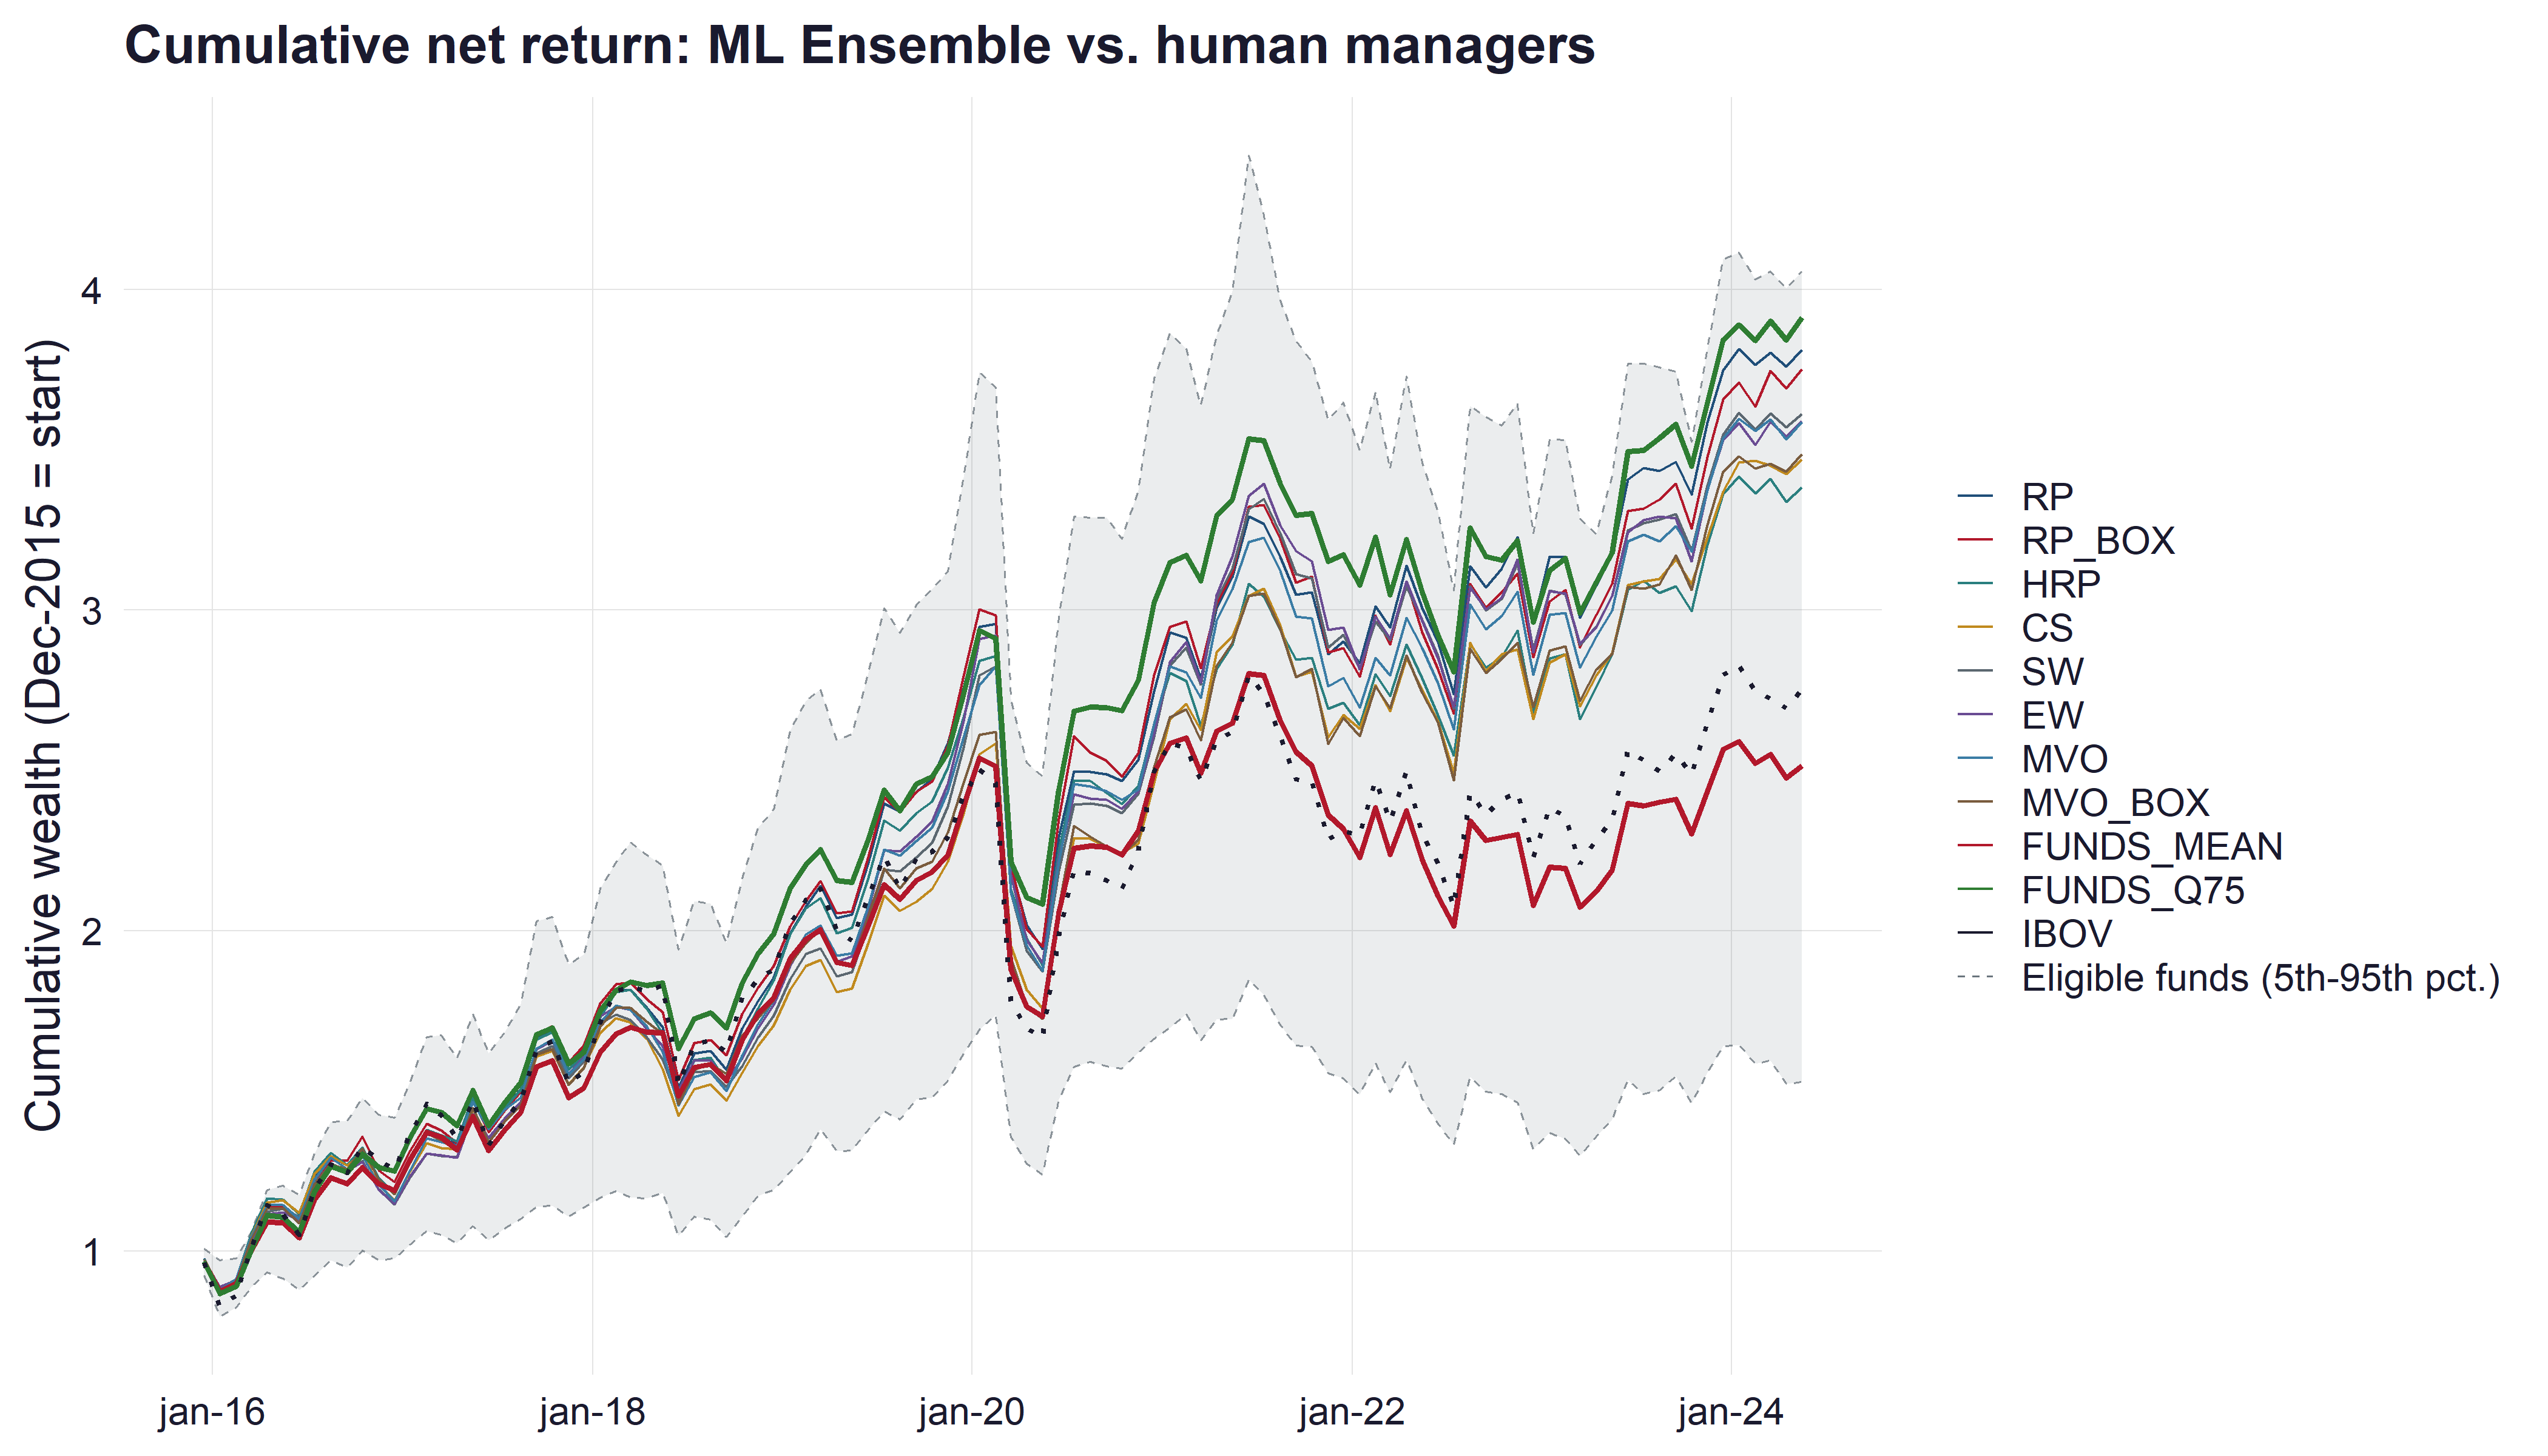
\includegraphics[width=\linewidth]{figures/cumulative_return.png}
\label{fig:cumret}
\end{figure}


\begin{figure}[htbp]
\centering
\captionsetup{
  justification=raggedright,
  labelsep=none,
  singlelinecheck=false,
  labelformat=boldlabel,
}
\caption[Net and gross feature importance by theme across ML models (last period).]{\footnotesize \textbf{: Net and gross feature importance by theme across ML models (last period).} Final-refit signed and gross surrogate loadings aggregated by characteristic theme. Loadings are normalized by each model's total absolute loading. Coloured bars show the signed net contribution and grey envelopes the gross contribution before within-theme cancellation.}
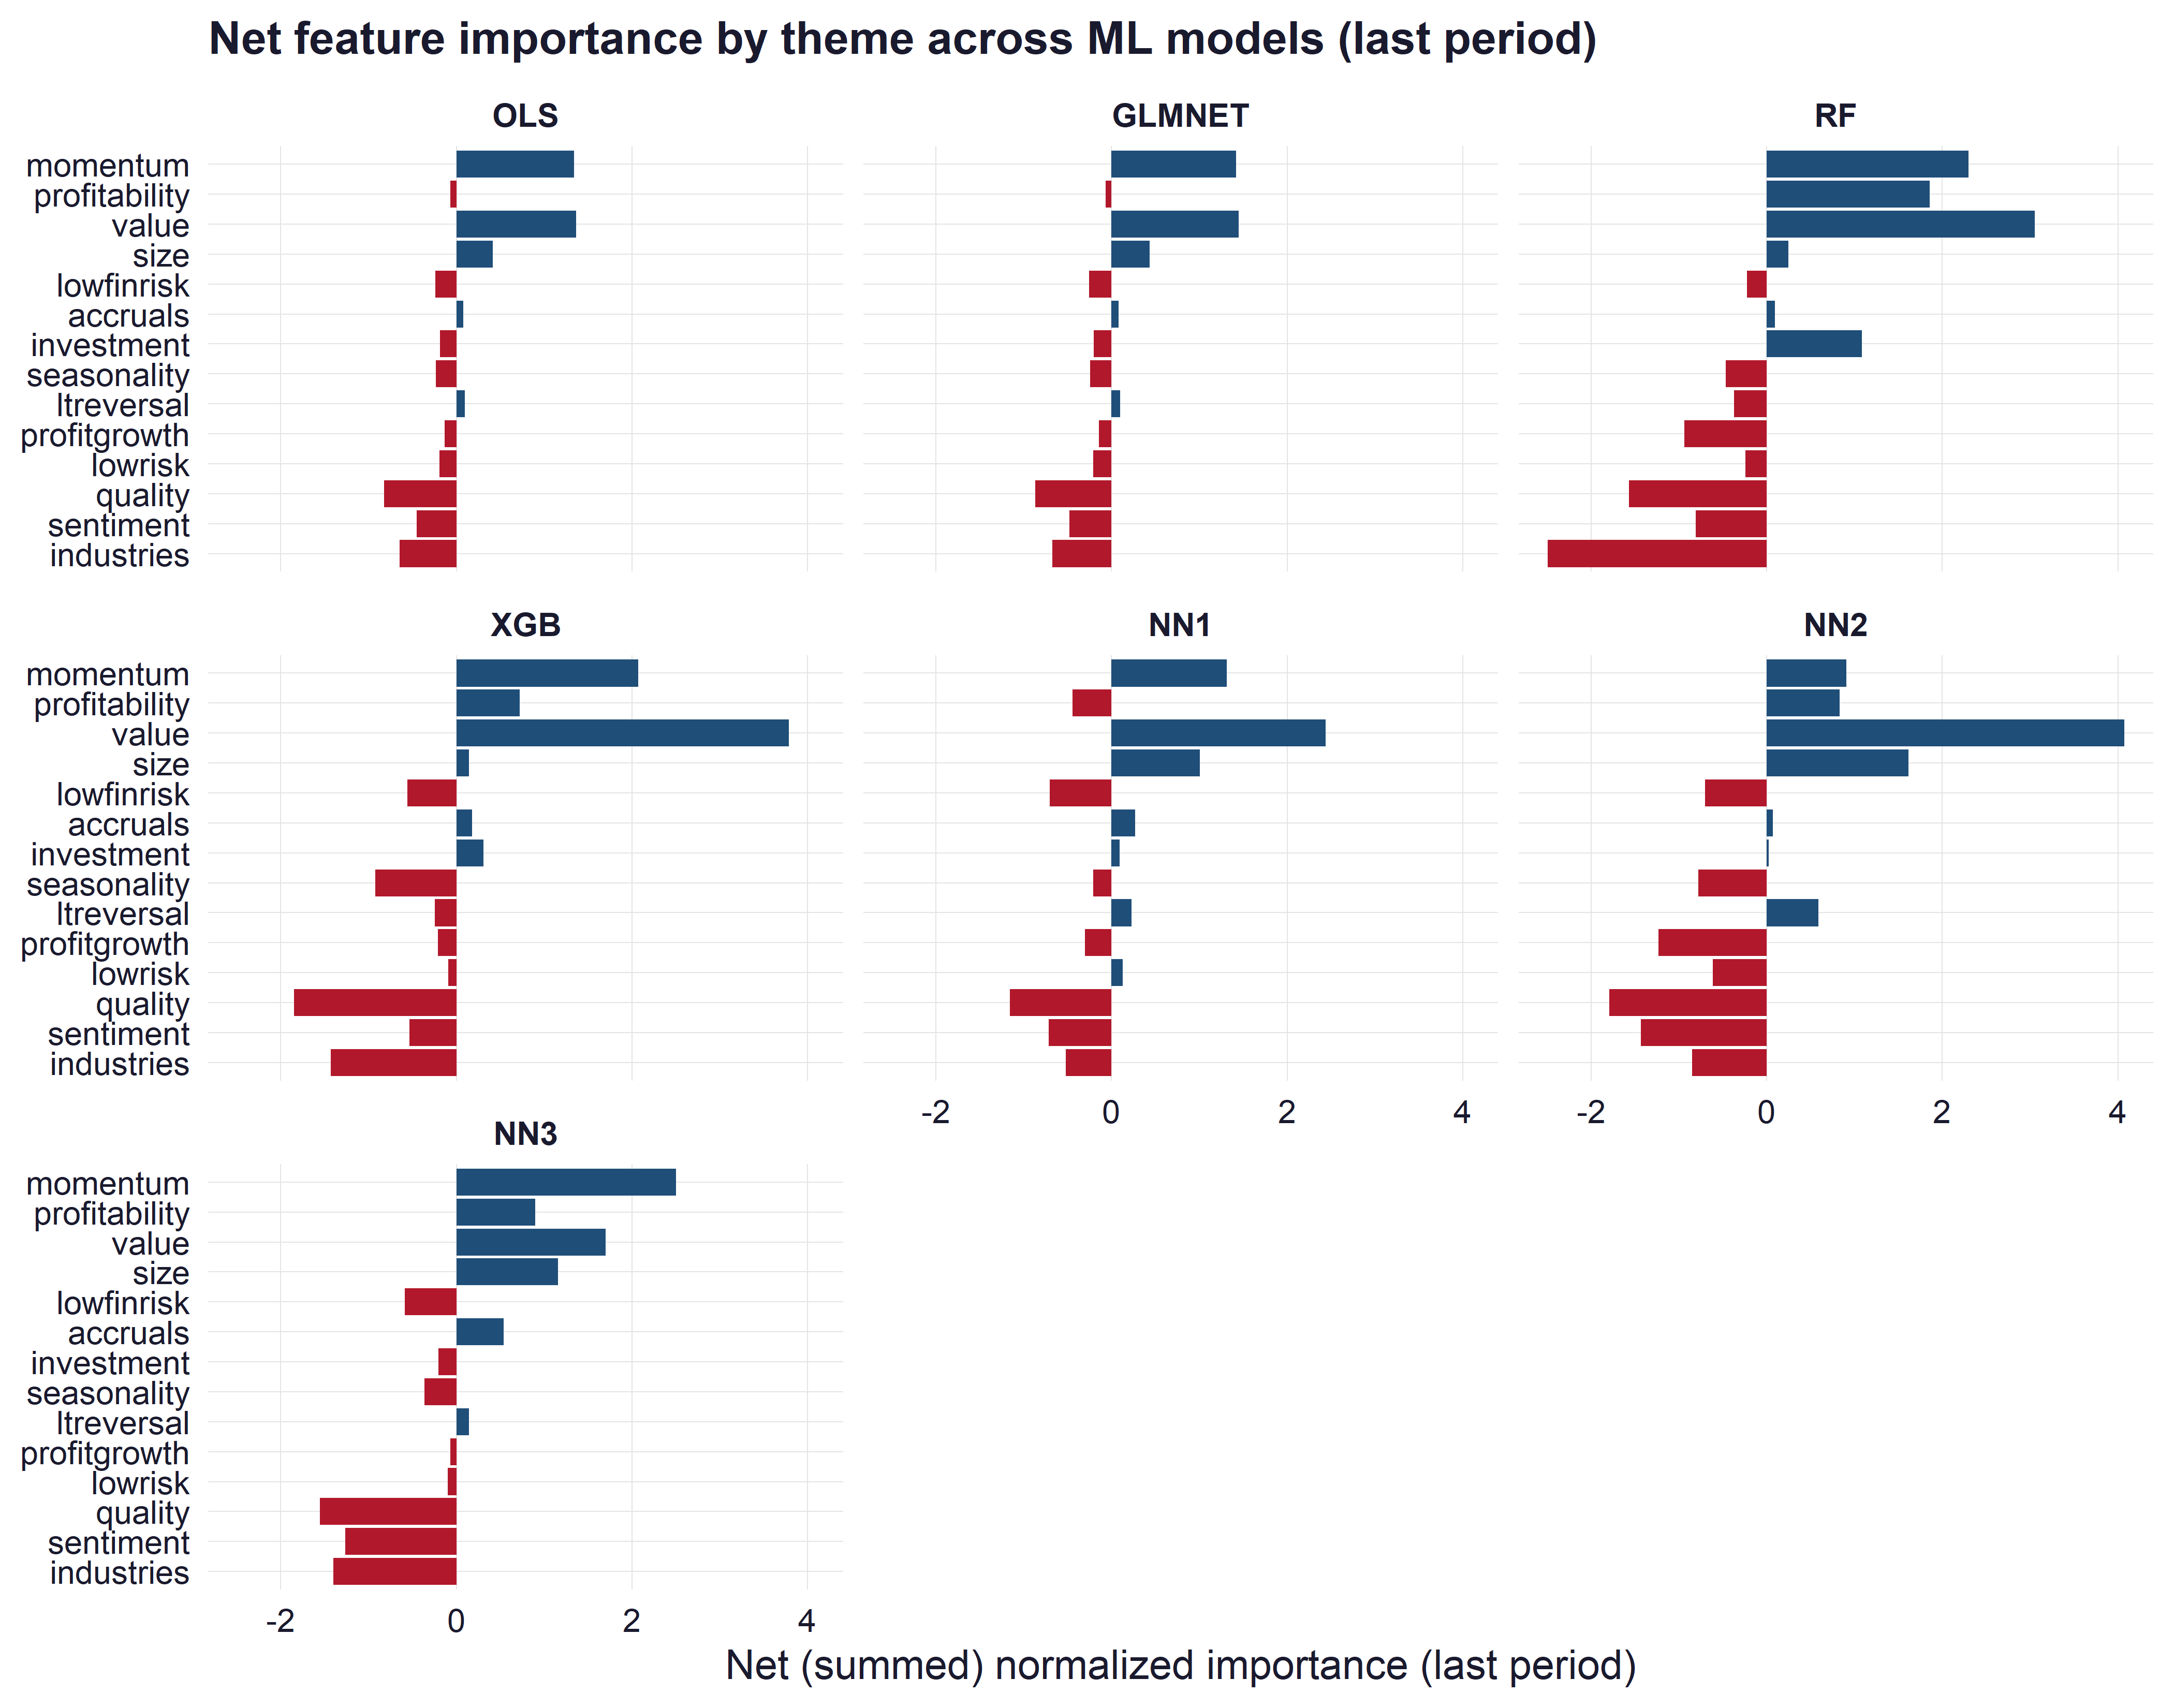
\includegraphics[width=\linewidth]{figures/feature_importance_bar.png}
\label{fig:fi_bar}
\end{figure}


\begin{figure}[htbp]
\centering
\captionsetup{
  justification=raggedright,
  labelsep=none,
  singlelinecheck=false,
  labelformat=boldlabel,
}
\caption[Figure 5: \footnotesize ]{\footnotesize \textbf{: Average portfolio characteristics over time.} Weighted-average stock characteristics of each ML-ensemble portfolio (sum of end-of-period portfolio weights times the characteristic) at every rebalance date. Each panel is one characteristic: Sharpe ratio (12m), earnings yield (NI/ME), return on equity (12m), gross profitability (GP/AT), dividend yield (36m median), return volatility (12m), log market capitalization, quality minus junk (QMJ) and the three-year change in FCF/BE. Each line is one portfolio-construction scheme (RP, RP\_BOX, HRP, CS, SW, EW, MVO, MVO\_BOX); the dashed black line is the IBOV benchmark's weighted average. Vertical scales differ across panels.}
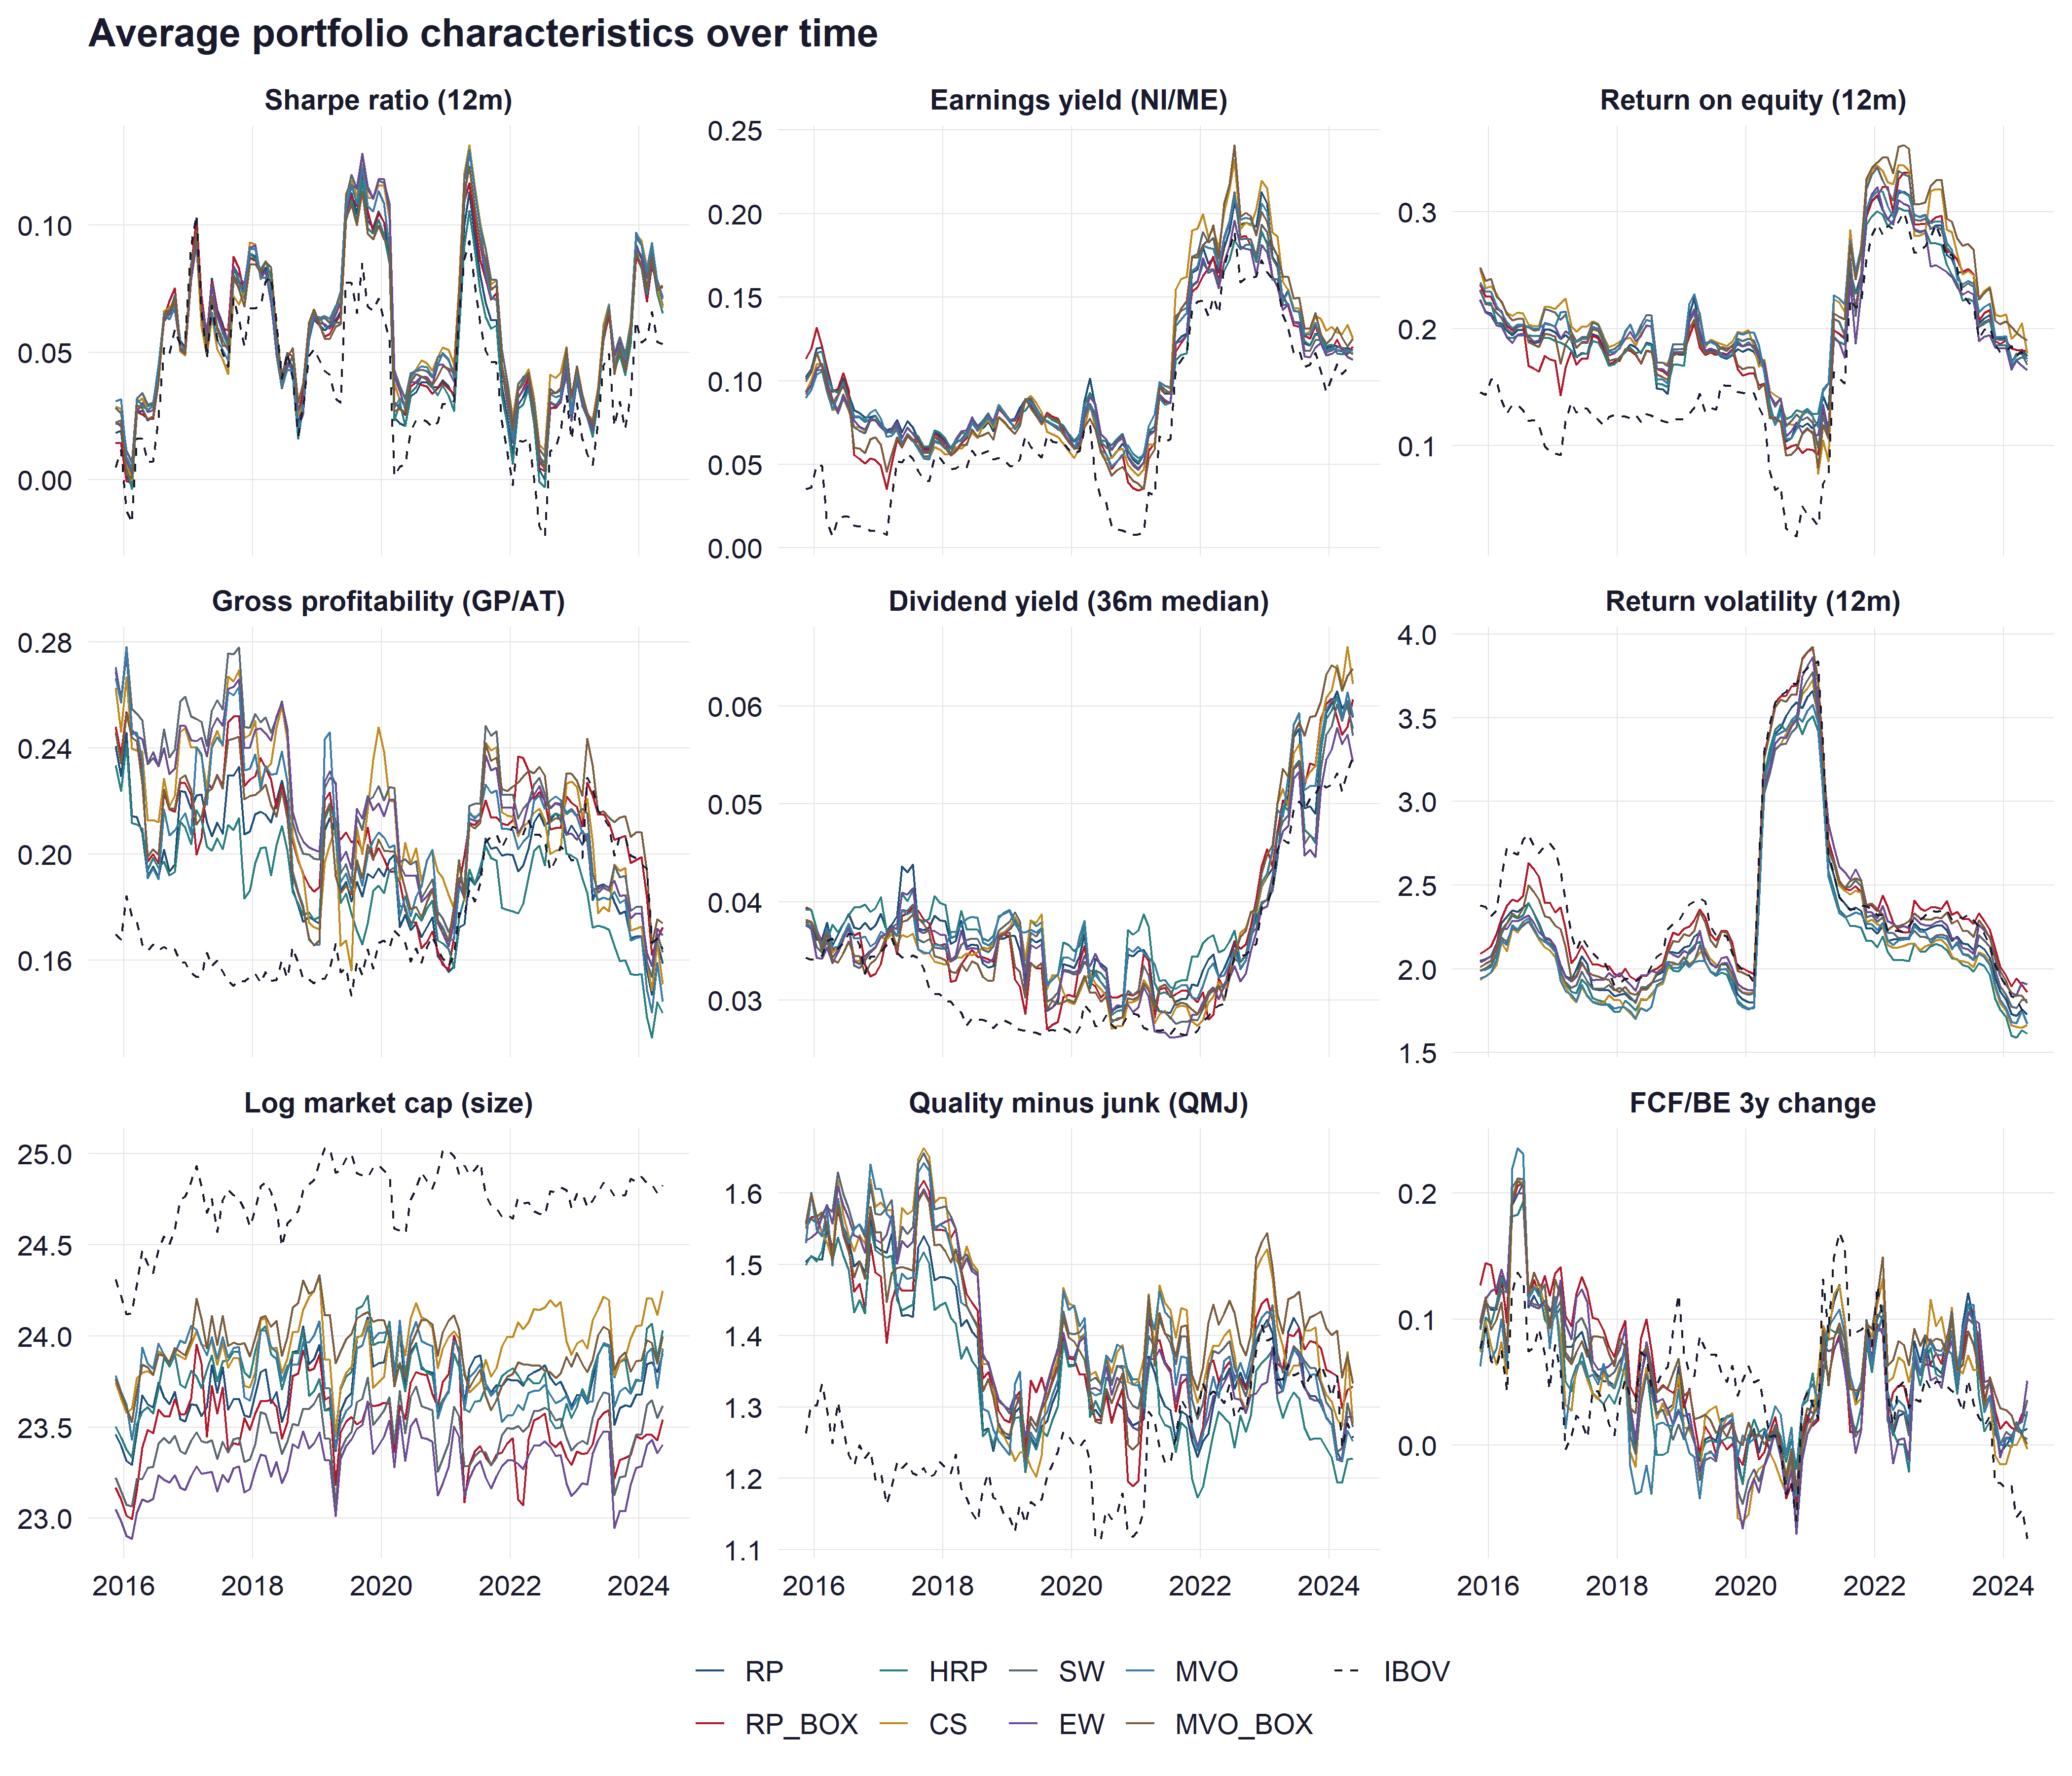
\includegraphics[width=\linewidth]{figures/portfolio_characteristics.png}
\label{fig:port_char}
\end{figure}


\input{../figures/gap_summary_figure.tex}

\begin{figure}[htbp]
\centering
\captionsetup{
  justification=raggedright,
  labelsep=none,
  singlelinecheck=false,
  labelformat=boldlabel,
}
\caption[Man and machine: active risk-return frontier.]{\footnotesize \textbf{: Man and machine: active risk-return frontier.} Annualized active return and risk for monthly rebalanced combinations holding $w$ in an ML Ensemble portfolio and $1-w$ in a human-manager benchmark. FUNDS\_MEAN and FUNDS\_Q75 are diversified fund portfolios; MED\_FUND and MED\_FUND\_Q75 report the median result across individual-fund combinations. In the two diversified panels the Information Ratio is the slope of a ray from the origin. In the two MED panels the coordinates are cross-fund medians of the components, so the slope is the median-component ratio and not the median of the fund-level Information Ratios reported in Table~\ref{combofront}. All returns are measured 15th-to-15th against IBOV. Squares, triangles and diamonds mark the pure manager, pure ML portfolio and maximum-IR combination. In the MED panels the $w=0$ square differs by ML scheme because months in which a fund does not report are held in that scheme's ML portfolio.}
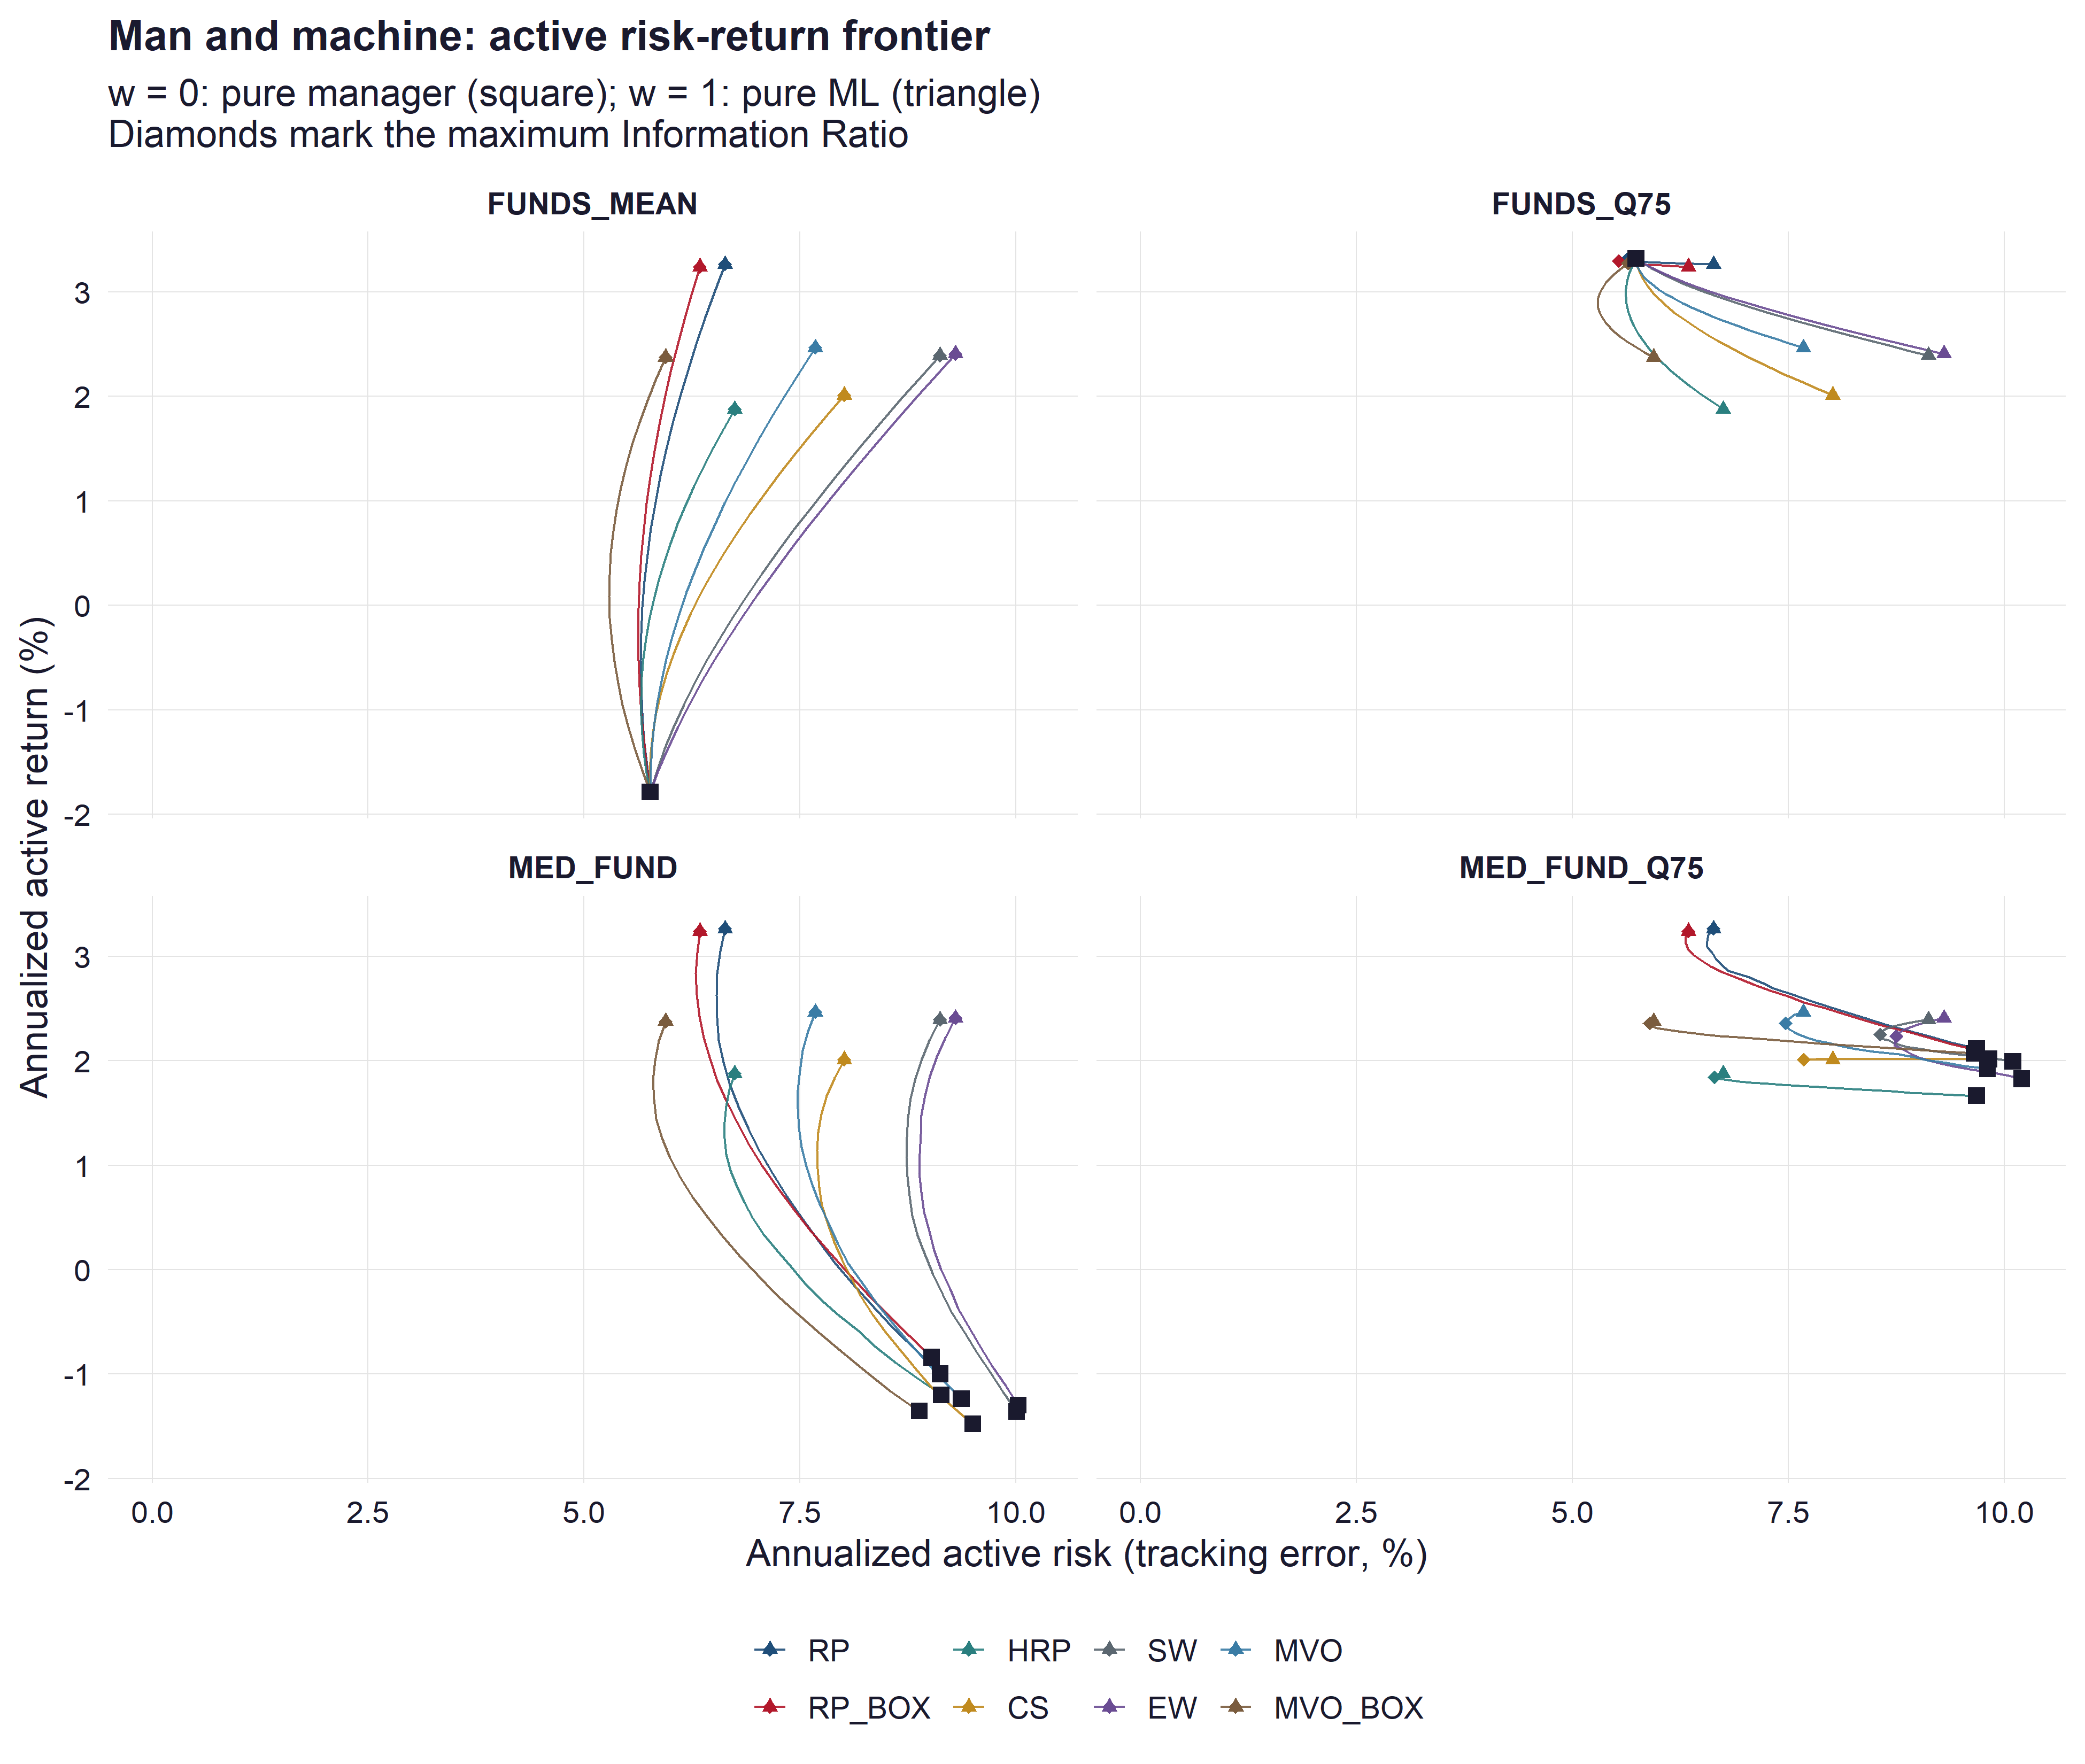
\includegraphics[width=\linewidth]{figures/combination_frontier.png}
\label{fig:combo_frontier}
\end{figure}


\clearpage

\section{Internet Appendix}

\setcounter{table}{0}
\renewcommand{\thetable}{IA.\arabic{table}}
\renewcommand{\theHtable}{IA.\arabic{table}}
\setcounter{figure}{0}
\renewcommand{\thefigure}{IA.\arabic{figure}}
\renewcommand{\theHfigure}{IA.\arabic{figure}}
\setcounter{equation}{0}
\renewcommand{\theequation}{IA.\arabic{equation}}
\renewcommand{\theHequation}{IA.\arabic{equation}}

\subsection{Algorithmic Details}\label{app:algorithmic}

This appendix provides the functional forms and implementation details for the prediction models summarized in Section~\ref{sec:methods}. Let $y_{i,t+h}$ denote the benchmark-relative three-month return and $\mathbf{z}_{i,t}$ the vector of characteristics available at month $t$. Models are estimated on the pooled panel using only information available at the formation date.

\subsection{Linear Models}

OLS estimates the linear benchmark
\begin{equation}
g_{\mathrm{OLS}}(\mathbf{z}_{i,t})=\mathbf{z}_{i,t}^{T}\boldsymbol{\theta}.
\end{equation}
ENET minimizes squared prediction error plus a mixture of L1 and L2 penalties:
\begin{multline}
\label{elasticeq}
\mathcal{L}_{\mathrm{ENET}}=
\frac{1}{N}\sum_{i,t}\left[y_{i,t+h}-g(\mathbf{z}_{i,t})\right]^2+
\lambda^{\psi}(1-\lambda^{\rho})\sum_j|\theta_j|+
\frac{1}{2}\lambda^{\psi}\lambda^{\rho}\sum_j\theta_j^2.
\end{multline}
The penalty-path floor $\lambda^{\psi}$ and ridge share $\lambda^{\rho}$ are selected at each refit.

\subsection{Tree Ensembles}

A regression tree partitions characteristic space into terminal regions $C_l$ and assigns each observation the mean outcome in its region:
\begin{equation}
g_{\mathrm{tree}}(\mathbf{z}_{i,t})=
\sum_{l=1}^{L}\theta_l\mathbf{1}\{\mathbf{z}_{i,t}\in C_l\}.
\end{equation}
RF averages trees grown on bootstrap samples, with a random fraction of characteristics considered at each split. This decorrelates trees and reduces variance. XGB instead constructs an additive sequence of trees,
\begin{equation}
\label{objxgb}
g_{\mathrm{XGB}}(\mathbf{z}_{i,t})=\sum_{f=1}^{F}T_f(\mathbf{z}_{i,t}),
\end{equation}
where each new tree is fitted to the remaining loss from the preceding ensemble. Tree depth governs interaction order, the learning rate scales the contribution of each new tree, and the number of trees controls the length of the boosting sequence. The regularized XGBoost objective also penalizes leaf complexity and leaf weights \citep{chenguestrin2016}.

\subsection{Neural Networks}

The neural-network models are feed-forward networks with ReLU activations,
\begin{equation}
\label{simplenn}
g_{\mathrm{NN}}(\mathbf{z}_{i,t})=
\mathbf{W}_{K}\operatorname{ReLU}\left(\cdots\operatorname{ReLU}
\left(\mathbf{W}_{1}\mathbf{z}_{i,t}+\mathbf{b}_{1}\right)\cdots\right)+\mathbf{b}_{K}.
\end{equation}
NN1 has one hidden layer with 32 units; NN2 has layers with 32 and 16 units; and NN3 has layers with 32, 16, and 8 units. The networks are trained with Adam, batch normalization, and dropout. The tuning grid varies the learning rate and L1 penalty; the other training settings are held fixed as reported in Table~\ref{hyperchoice}. After hyperparameter selection, each architecture is refitted from ten independent random initializations ($n_{\mathrm{ensembles}}=10$) and the predictions are averaged, following \citet{gukellyxiu2020}. This reduces sensitivity to a single initialization without increasing the tuning budget, because tuning itself uses one fitted network. The loss combines squared error and the L1 penalty,
\begin{equation}
\label{objnn}
\mathcal{L}_{\mathrm{NN}}=
\sum_{i,t}\left[y_{i,t+1}-g_{\mathrm{NN}}(\mathbf{z}_{i,t})\right]^2+
\lambda^{\omega}\sum_k\left\|\mathbf{W}_k\right\|_1.
\end{equation}

\subsection{Ensembles and Interpretation}

The cross-model ensemble forecast is the equal-weighted mean of its constituent forecasts and is distinct from the within-architecture averaging of independently initialized neural networks. Feature interpretation is based exclusively on the GSM: at each refit, a linear surrogate is fitted to a model's predictions using the full characteristic set, and its normalized coefficients provide a common approximation of the prediction function across model classes.

\subsection{Portfolio Construction}

\subsubsection{Portfolio Formation and Common Inputs}

Let $\mathcal{S}_{t}$ denote the investable set at formation date $t$. The ML forecast is first used to rank stocks within each mandate, retaining the upper tercile,
\begin{equation}
\mathcal{S}_{t}=\left\{s:\widehat{EXR}_{s,t+h}\geq
Q_{0.67}\left(\widehat{EXR}_{t+h}\right)\right\},
\end{equation}
Forecasts affect all portfolios through this eligibility rule. Their magnitudes also enter SW, CS, MVO, and MVO\_BOX, whereas RP, RP\_BOX, and HRP use the forecasts only to determine $\mathcal{S}_{t}$.

The meta-model first portfolio formation date is November 2015. Portfolios rebalance in February, April, May, August, and November, thereby concentrating trades around the arrival of accounting information while limiting unnecessary turnover. All specifications are long-only and fully invested. The liquidity floor excludes stocks below the micro-cap threshold defined in Section~\ref{sec:methods}.

The covariance-based methods use active daily returns relative to the mandate benchmark. The covariance matrix is estimated with the configured 126-day lookback and linear shrinkage toward a constant-correlation target \citep{ledoitwolf2003,ledoitwolf2004}. A sample covariance matrix is particularly sensitive to estimation error when the cross-section is large relative to the available history, while extending the window indefinitely is also unattractive when return dependence changes over time. Constant-correlation shrinkage provides a more stable compromise between sampling variation and a parsimonious target. The same estimator is supplied to RP, RP\_BOX, HRP, MVO, and MVO\_BOX. All eight portfolio methods also use the same transaction-cost parameters: a 7 bps direct cost, strategy AUM of 150 BRL million, square-root market impact with $\alpha=0.5$, and dynamic impact scaling \citep{barra1997}.

\subsubsection{Heuristic Portfolios}

The heuristic portfolios are Equal-Weighted (EW), Signal-Weighted (SW), and Cap-Scaled (CS), which envolve simple rules rather than complex algorithms. They do not use the covariance matrix to determine weights \citep{ghayurheaneyplatt2019} and EW ignores even the expected returns vector, thus SW and CS use both forecast rank and forecast magnitude, while EW uses only the eligible set. Overall, they provide transparent benchmarks for separating gains from stock selection from gains that may arise through explicit risk modelling. Let $q_{s,t}$ denote the positive expected-return score passed to portfolio construction and let $c_{s,t}$ denote the transformed inflation-adjusted three-month average daily trading value. For $s\in\mathcal{S}_{t}$, weights are
\begin{align}
w_{s,t}^{EW} &= \frac{1}{|\mathcal{S}_{t}|},\\
w_{s,t}^{SW} &= \frac{q_{s,t}}{\sum_{j\in\mathcal{S}_{t}}q_{j,t}},\\
w_{s,t}^{CS} &= \frac{q_{s,t}c_{s,t}}
{\sum_{j\in\mathcal{S}_{t}}q_{j,t}c_{j,t}}.
\end{align}
The capacity score $c_{s,t}$ is obtained by winsorizing the liquidity metric at the 2.5th and 97.5th percentiles, standardizing it, and applying a positive monotone transformation.

\subsubsection{Risk-Parity Portfolios}

Risk-parity portfolios are widely used in empirical applications because they avoid direct estimation of expected returns and distribute portfolio risk rather than capital uniformly \citep{chavesetal2011}. Risk parity assigns the same risk budget $b_s=1/|\mathcal{S}_{t}|$ to each eligible stock. With covariance matrix $\widehat{\boldsymbol{\Sigma}}_{t}$, the component contribution of stock $s$ to portfolio variance is
\begin{equation}
r_{s,t}=w_{s,t}
\left(\widehat{\boldsymbol{\Sigma}}_{t}\mathbf{w}_{t}\right)_{s}.
\end{equation}
The equal-risk-budget conditions are
\begin{equation}
w_{s,t}\left(\widehat{\boldsymbol{\Sigma}}_{t}\mathbf{w}_{t}\right)_{s}
=b_s\mathbf{w}_{t}^{T}\widehat{\boldsymbol{\Sigma}}_{t}\mathbf{w}_{t},
\qquad s\in\mathcal{S}_{t}.
\end{equation}

For RP, the implementation follows the convex formulation of \citet{spinu2013}. Defining
$\mathbf{x}_{t}=\mathbf{w}_{t}/
\sqrt{\mathbf{w}_{t}^{T}\widehat{\boldsymbol{\Sigma}}_{t}\mathbf{w}_{t}}$,
the optimization problem is
\begin{equation}
\underset{\mathbf{x}_{t}>0}{\operatorname{minimize}}\quad
\frac{1}{2}\mathbf{x}_{t}^{T}\widehat{\boldsymbol{\Sigma}}_{t}\mathbf{x}_{t}
-\mathbf{b}^{T}\log(\mathbf{x}_{t}),
\end{equation}
and recovers portfolio weights as
$\mathbf{w}_{t}=\mathbf{x}_{t}/(\mathbf{1}^{T}\mathbf{x}_{t})$.
The selected cyclical algorithm implementation updates one coordinate at a time. If
$a_{s,t}=\sum_{j\neq s}\widehat{\Sigma}_{sj,t}x_{j,t}$, its positive coordinate update is
\begin{equation}
x_{s,t}\leftarrow
\frac{-a_{s,t}+
\sqrt{a_{s,t}^{2}+4\widehat{\Sigma}_{ss,t}b_s}}
{2\widehat{\Sigma}_{ss,t}}.
\end{equation}
These updates continue until the objective tolerance is satisfied, after which the vector is normalized to sum to one \citep{spinu2013}.

RP\_BOX is a different numerical problem rather than the same closed-form allocation with weights clipped afterward. Its feasible set imposes the benchmark-relative bounds
\begin{equation}
\max\{w_{s,b,t}-0.05,0\}\leq w_{s,t}\leq
\min\{w_{s,b,t}+0.05,1\},
\qquad \mathbf{1}^{T}\mathbf{w}_{t}=1.
\end{equation}
The unconstrained cyclical solution provides the initial point. The box bounds move the problem outside the convex log-barrier formulation above, so the bounded problem is instead solved by successive convex approximation of
\begin{equation}
R(\mathbf{w}_{t})=
\sum_{s\in\mathcal{S}_{t}}
\left[
\frac{w_{s,t}
\left(\widehat{\boldsymbol{\Sigma}}_{t}\mathbf{w}_{t}\right)_{s}}
{\mathbf{w}_{t}^{T}\widehat{\boldsymbol{\Sigma}}_{t}\mathbf{w}_{t}}
-b_s
\right]^2
\end{equation}
over the bounded simplex. At each iteration, the risk-concentration residuals are locally approximated, a proximal quadratic program is solved under the box and budget constraints, and the weights are updated with a damped step. This is the successive convex risk-parity procedure of \citet{fengpalomar2015}, rather than an ex-post truncation of the unconstrained solution.

\subsubsection{Hierarchical Risk Parity}

HRP follows \citet{lopezdeprado2016}. The implementation first converts the shrunk correlation matrix into the distance matrix
\begin{equation}
d_{ij,t}=\sqrt{\frac{1-\rho_{ij,t}}{2}},
\end{equation}
and applies single-linkage hierarchical clustering to the Euclidean distances between the rows of $\mathbf{D}_{t}$. The resulting dendrogram determines a quasi-diagonal ordering. Recursive bisection then divides the ordered assets into two clusters. Within each cluster $C$, inverse-variance weights are used to estimate cluster variance,
\begin{equation}
\widetilde{\mathbf{w}}_{C}\propto
\operatorname{diag}\left(\widehat{\boldsymbol{\Sigma}}_{C,t}\right)^{-1},
\qquad
\widehat{\sigma}^{2}_{C,t}=
\widetilde{\mathbf{w}}_{C}^{T}
\widehat{\boldsymbol{\Sigma}}_{C,t}
\widetilde{\mathbf{w}}_{C}.
\end{equation}
For left and right clusters $L$ and $R$, the capital share assigned to $L$ is
\begin{equation}
\alpha_{L,t}=
\frac{\widehat{\sigma}^{2}_{R,t}}
{\widehat{\sigma}^{2}_{L,t}+\widehat{\sigma}^{2}_{R,t}},
\end{equation}
with $1-\alpha_{L,t}$ assigned to $R$. The procedure is repeated until each branch contains one stock. HRP therefore uses the ML model for eligibility but not as an expected-return tilt.

\subsubsection{Optimal Mean-Tracking-Error Portfolios}

MVO adapts the mean-variance tangency portfolio to benchmark-relative expected returns and risk. For eligible stocks, the objective is
\begin{equation}
\underset{\mathbf{w}_{t}}{\operatorname{maximize}}\quad
\frac{\mathbf{w}_{t}^{T}\widehat{\mathbf{q}}_{t+h}}
{\sqrt{\mathbf{w}_{t}^{T}
\widehat{\boldsymbol{\Sigma}}_{t}\mathbf{w}_{t}}},
\qquad
\mathbf{1}^{T}\mathbf{w}_{t}=1,\quad \mathbf{w}_{t}\geq0,
\end{equation}
where $\widehat{\mathbf{q}}_{t+h}$ is the vector of ML expected-return scores. This is the tangency allocation in mean-tracking-error space. Its economic appeal is accompanied by a familiar practical limitation: estimated tangency portfolios can be highly concentrated and unstable because expected returns and covariances are measured with error. The implementation samples 1,000 feasible random portfolios and retains the portfolio with the largest expected Information Ratio.

To reduce sensitivity to estimation error, this search is repeated under 50 perturbed input sets \citep{michaud1989}. Expected-return scores receive independent Gaussian noise with standard deviation $0.5$ times the cross-sectional standard deviation of the score. The covariance eigenvectors are retained, while each eigenvalue is multiplied by an independent lognormal perturbation $\exp(\varepsilon)$, with $\varepsilon\sim N(0,0.25^2)$. The final allocation is the equal-weighted average of the base solution and the 50 perturbed solutions.

MVO\_BOX addresses concentration and trading feasibility directly. It applies the same benchmark-relative 5\% individual-weight bounds as RP\_BOX, and, in addition, retains a 10\% quantile-range buffer, restricting changes buffered stocks to 1\% for micro-caps and 2.5\% for small-caps.

\clearpage

\subsection{Additional Tables}

\input{../tables/implementation_robustness.tex}

\input{../tables/gap_market_states.tex}

\input{../tables/gap_flow_scale.tex}

\input{../tables/gap_mediators.tex}

\begin{table}[p]
\captionsetup{justification=raggedright,labelsep=none,singlelinecheck=false,labelformat=boldlabel}
\renewcommand{\arraystretch}{1.02}
\caption[Fund-picking robustness of the RP--human frontier]{\footnotesize \textbf{: Fund-picking robustness of the RP--human frontier.} RP is the pre-specified ML portfolio because it is a transparent, risk-controlled ensemble; it was not selected because it produced the strongest result. ML returns are net of transaction costs and the 1\% annual management fee. All Information Ratios use 15th-to-15th monthly returns and the IBOV as benchmark, and are computed as the annualized arithmetic mean active return divided by the tracking error, matching Table~\ref{combofront} rather than the geometric convention of Table~\ref{actret}. Panel A ranks funds over the full evaluation window and varies the retained top share. Human IR and RP IR are standalone values; Best IR is the maximum over RP--human weights from zero to one in five-percentage-point increments, and $w^{*}$ is the corresponding RP weight. $\Delta$IR is Best IR minus the better standalone IR. Because the weight grid contains both endpoints, $\Delta$IR is non-negative by construction and is inflated by the maximization over the grid; the bracket is therefore a percentile band for a bounded statistic, not a two-sided significance interval, and a lower bound of 0.00 carries no test of a null. Bands come from 999 joint circular 12-month block-bootstrap samples, with funds re-ranked inside every sample. Panel B draws 1,000 fixed equal-weight baskets without replacement from the ex-post top quartile. P5 and P95 describe basket-selection dispersion, not confidence intervals. Panel C uses 500 baskets per cell and controls the fraction selected from the ex-post top quartile; Min. positive is the lowest precision with positive median $\Delta$IR, which is equivalent to $P(\Delta\mathrm{IR}>0)>50\%$ because $\Delta$IR is non-negative by construction; Min. likely is the stricter crossing at $P(\Delta\mathrm{IR}>0)\geq 75\%$. The final row replaces full-window ranking with a trailing 12-month, past-only top-quartile rule.}
\scriptsize
\setlength{\tabcolsep}{3pt}
\begin{tabularx}{\linewidth}{>{\raggedright\arraybackslash}m{1.7cm}*{7}{>{\raggedleft\arraybackslash}X}}
\hline
\multicolumn{8}{l}{\textit{Panel A: oracle top-share sensitivity (RP)}} \\
Top share & Funds & Human IR & RP IR & Best IR & $\Delta$IR & $w^{*}$ & 95\% band $\Delta$IR \\
\hline
50\% & 564 & 0.12 & 0.49 & 0.49 & 0.00 & 100\% & [0.00, 0.03] \\
35\% & 395 & 0.36 & 0.49 & 0.49 & 0.00 & 100\% & [0.00, 0.06] \\
25\% & 282 & 0.58 & 0.49 & 0.59 & 0.01 & 20\% & [0.00, 0.06] \\
15\% & 170 & 0.93 & 0.49 & 0.93 & 0.00 & 0\% & [0.00, 0.07] \\
10\% & 113 & 1.27 & 0.49 & 1.27 & 0.00 & 0\% & [0.00, 0.08] \\
5\% & 57 & 1.72 & 0.49 & 1.72 & 0.00 & 0\% & [0.00, 0.11] \\
\hline
\multicolumn{8}{l}{\textit{Panel B: fixed baskets sampled from the oracle top quartile}} \\
Funds & Draws & Median best & P5 & P95 & Median $\Delta$IR & $P(\Delta>0)$ & \\
\hline
1 & 1000 & 0.49 & 0.49 & 0.87 & 0.00 & 47\% & \\
2 & 1000 & 0.49 & 0.49 & 0.90 & 0.00 & 51\% & \\
3 & 1000 & 0.50 & 0.49 & 0.93 & 0.00 & 56\% & \\
5 & 1000 & 0.50 & 0.49 & 0.86 & 0.01 & 62\% & \\
10 & 1000 & 0.52 & 0.49 & 0.89 & 0.01 & 70\% & \\
20 & 1000 & 0.54 & 0.49 & 0.86 & 0.01 & 76\% & \\
50 & 1000 & 0.57 & 0.49 & 0.78 & 0.01 & 83\% & \\
100 & 1000 & 0.58 & 0.50 & 0.72 & 0.01 & 88\% & \\
All (282) & 1 & 0.59 & 0.59 & 0.59 & 0.01 & 100\% & \\
\hline
\multicolumn{8}{l}{\textit{Panel C: calibrated picker precision}} \\
Funds & Min. positive & Min. likely & $\Delta$IR at 100\% & & & & \\
\hline
4 & 100\% & -- & 0.01 & & & & \\
8 & 100\% & -- & 0.01 & & & & \\
20 & 100\% & 100\% & 0.01 & & & & \\
40 & 100\% & 100\% & 0.01 & & & & \\
\hline
\multicolumn{8}{l}{\textit{Past-only Q75 (12m, $T=90$): Human 0.25; Best 0.72; $\Delta$IR 0.00; $w^{*}$ 100\%.}} \\
\hline
\end{tabularx}
\label{fundpickerrobust}
\end{table}


\input{../tables/variable_definitions.tex}

\begin{table}[h]
\captionsetup{
  justification=raggedright,
  labelsep=none,
  singlelinecheck=false,
  labelformat=boldlabel,
}
\renewcommand{\arraystretch}{1.25}
\caption[Bayesian-optimization search space]{\footnotesize \textbf{: Bayesian-optimization search space.} Each entry is the closed interval searched for that hyperparameter; "--" means the hyperparameter does not apply to that model. Bounds are read directly from the tuning configuration stored with each fitted base learner, so they describe the search that was actually run. Hyperparameters are re-optimized at every walk-forward refit, so the table reports the domain rather than a selected value; Figure~\ref{fig:hyper_time} shows the chosen values over time. OLS is unregularized and has no tuned hyperparameters. NN1--NN3 share one search space and differ only in depth. Symbols follow the notation of Section~\ref{sec:methods}; the mixing weight $\lambda^{\rho}$ of Equation~\ref{elasticeq} is the ridge share, which is one minus \texttt{glmnet}'s \texttt{alpha} and therefore searched over the same interval. The penalty path floor is \texttt{lambda.min.ratio}, the ratio of the smallest to the largest $\lambda^{\psi}$ on the fitted path, not $\lambda^{\psi}$ itself. Integer-valued hyperparameters are searched on the integers within the stated interval. The final rows give the search budget: the size of the initial space-filling design and the number of subsequent acquisition steps, per refit.}
\scriptsize
\setlength{\tabcolsep}{4pt}
\begin{tabularx}{\linewidth}{>{\raggedright\arraybackslash}m{5.0cm}>{\hsize=0.920\hsize\raggedleft\arraybackslash}X>{\hsize=0.920\hsize\raggedleft\arraybackslash}X>{\hsize=0.920\hsize\raggedleft\arraybackslash}X>{\hsize=1.241\hsize\raggedleft\arraybackslash}X}
\hline
Hyperparameter & ENET & RF & XGB & NN1--NN3 \\
\hline
Penalty path floor $\lambda^{\psi}$ & [$10^{-4}$, 0.5] & -- & -- & -- \\
L1/L2 mixing $\lambda^{\rho}$ & [0, 1] & -- & -- & -- \\
Trees / boosting rounds $\lambda^{T}$, $\lambda^{F}$ & -- & [200, 800] & [100, 400] & -- \\
Maximum depth $\lambda^{D}$ & -- & [2, 10] & [2, 5] & -- \\
Minimum terminal node size $\lambda^{L}$ & -- & [1, 10] & [1, 4] & -- \\
Feature subsampling fraction $\lambda^{R}$ & -- & [0.1, 1] & [0.6, 1] & -- \\
Row subsampling fraction $\lambda^{S}$ & -- & -- & [0.75, 1] & -- \\
Learning rate & -- & -- & [0.02, 0.07] & [$10^{-4}$, 0.01] \\
L1 penalty & -- & -- & [0, 1] & [$10^{-5}$, 0.01] \\
L2 penalty & -- & -- & -- & [$10^{-5}$, $10^{-3}$] \\
Minimum split loss & -- & -- & [0, 1.5] & -- \\
Dropout rate & -- & -- & -- & [0.25, 0.75] \\
Batch size $\lambda^{b}$ & -- & -- & -- & [128, 512] \\
Epochs $\lambda^{e}$ & -- & -- & -- & [60, 110] \\
\hline
Initial design points & 8 & 16 & 32 & 24 \\
Acquisition iterations & 4 & 8 & 16 & 12 \\
\hline
\multicolumn{5}{@{}p{0.98\linewidth}@{}}{\textit{Acquisition function: EI. Objective: validation RMSE over a 36-month validation window.}} \\
\hline
\end{tabularx}
\label{hyperchoice}
\end{table}


\clearpage

\subsection{Additional Figures}

\input{../figures/model_rmse_over_time_figure.tex}

\input{../figures/implementation_robustness_figure.tex}

\begin{figure}[htbp]
\centering
\captionsetup{
  justification=raggedright,
  labelsep=none,
  singlelinecheck=false,
  labelformat=boldlabel,
}
\caption[Figure 8: \footnotesize ]{\footnotesize \textbf{: Selected hyperparameters over time.} Bayesian-tuned hyperparameter values chosen at each walk-forward refit, for every tuned ML model (GLMNET, RF, XGB, NN1--NN3; OLS is untuned and omitted). Hyperparameters that play the same role across models share a panel and are drawn as separate coloured lines: number of trees (RF num.trees, XGB nrounds), maximum tree depth, minimum leaf size (RF min.bucket, XGB min\_child\_weight), learning rate (XGB eta, NN lr), early-stopping iteration and feature subsampling (RF mtry, XGB colsample\_bytree; both fractions of the features sampled). Model-specific hyperparameters keep their own panels, and the three neural networks share each remaining NN panel. Points are the selected values at each refit date; vertical scales differ across panels. Estimated on the individual-signals run.}
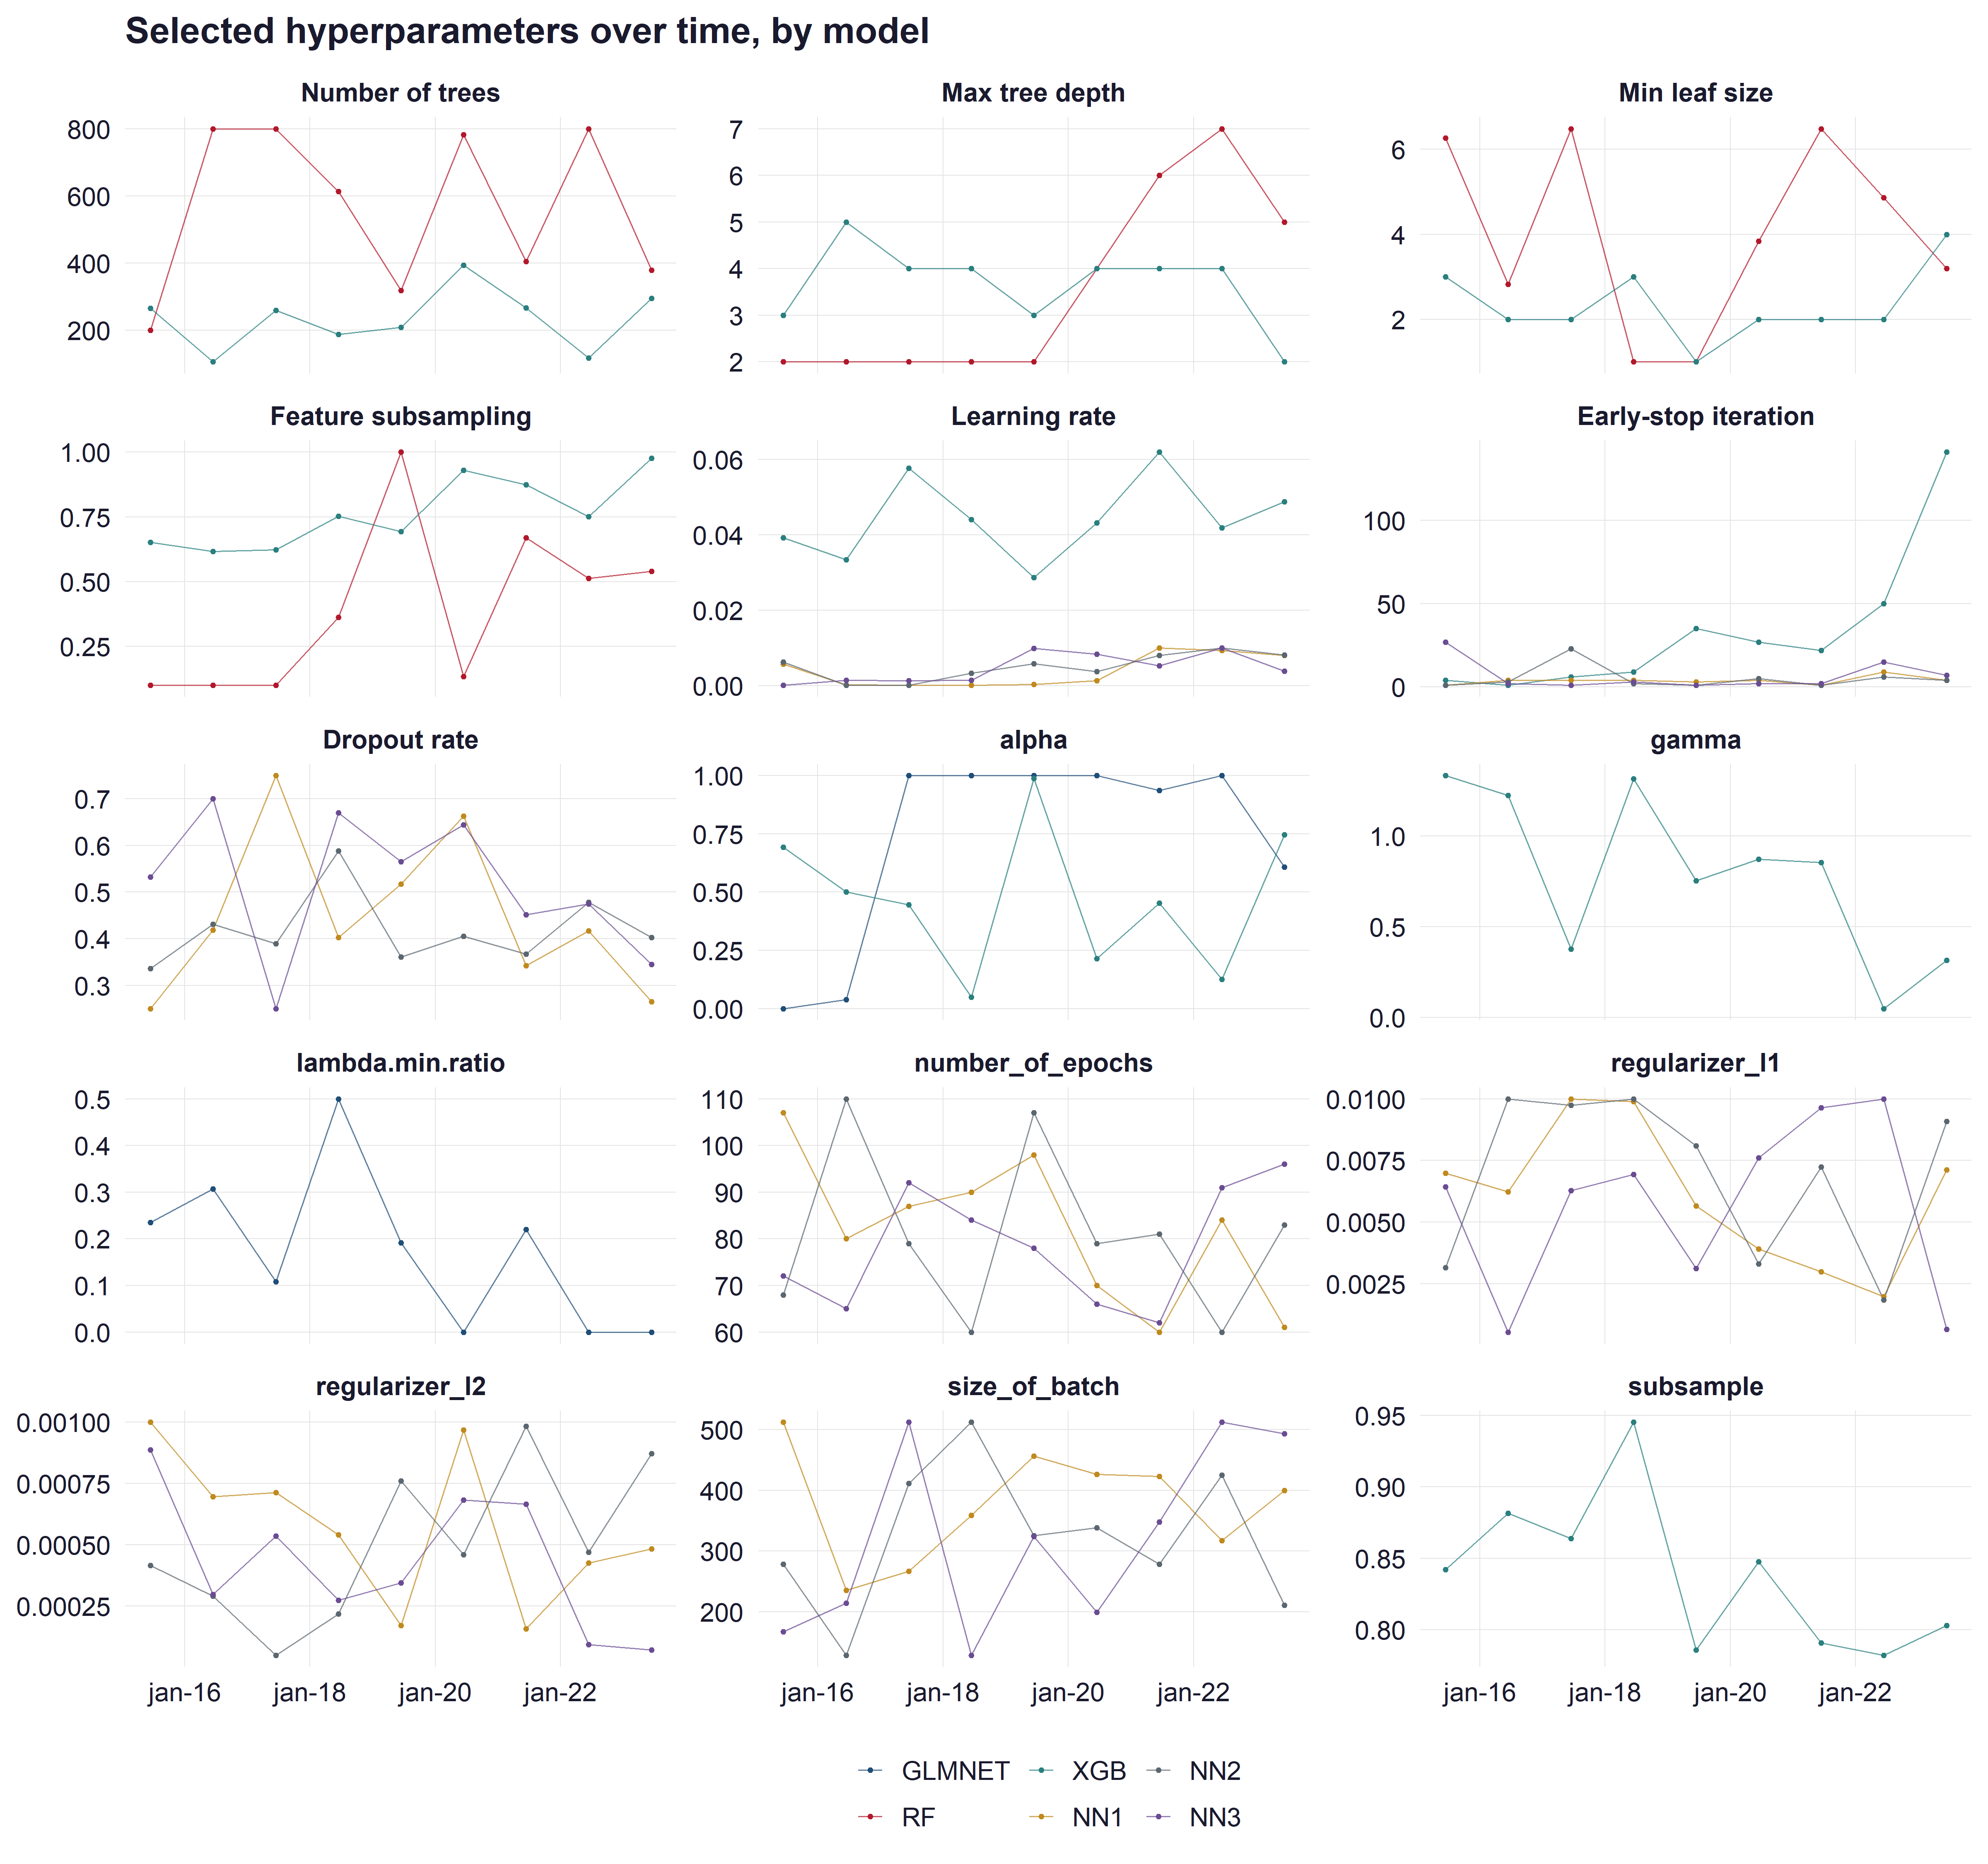
\includegraphics[width=\linewidth]{figures/hyperparameters_over_time.png}
\label{fig:hyper_time}
\end{figure}


\input{../figures/bh_eligibility_figure.tex}

\input{../figures/fund_industry_descriptives_figure.tex}

\begin{figure}[htbp]
\centering
\captionsetup{
  justification=raggedright,
  labelsep=none,
  singlelinecheck=false,
  labelformat=boldlabel,
}
\caption[Net feature importance by theme over time across ML models.]{\footnotesize \textbf{: Net feature importance by theme over time across ML models.} Signed surrogate loadings aggregated by characteristic theme at each refit. Loadings are normalized by each model's total gross loading. Colour records the direction and relative magnitude of the theme contribution.}
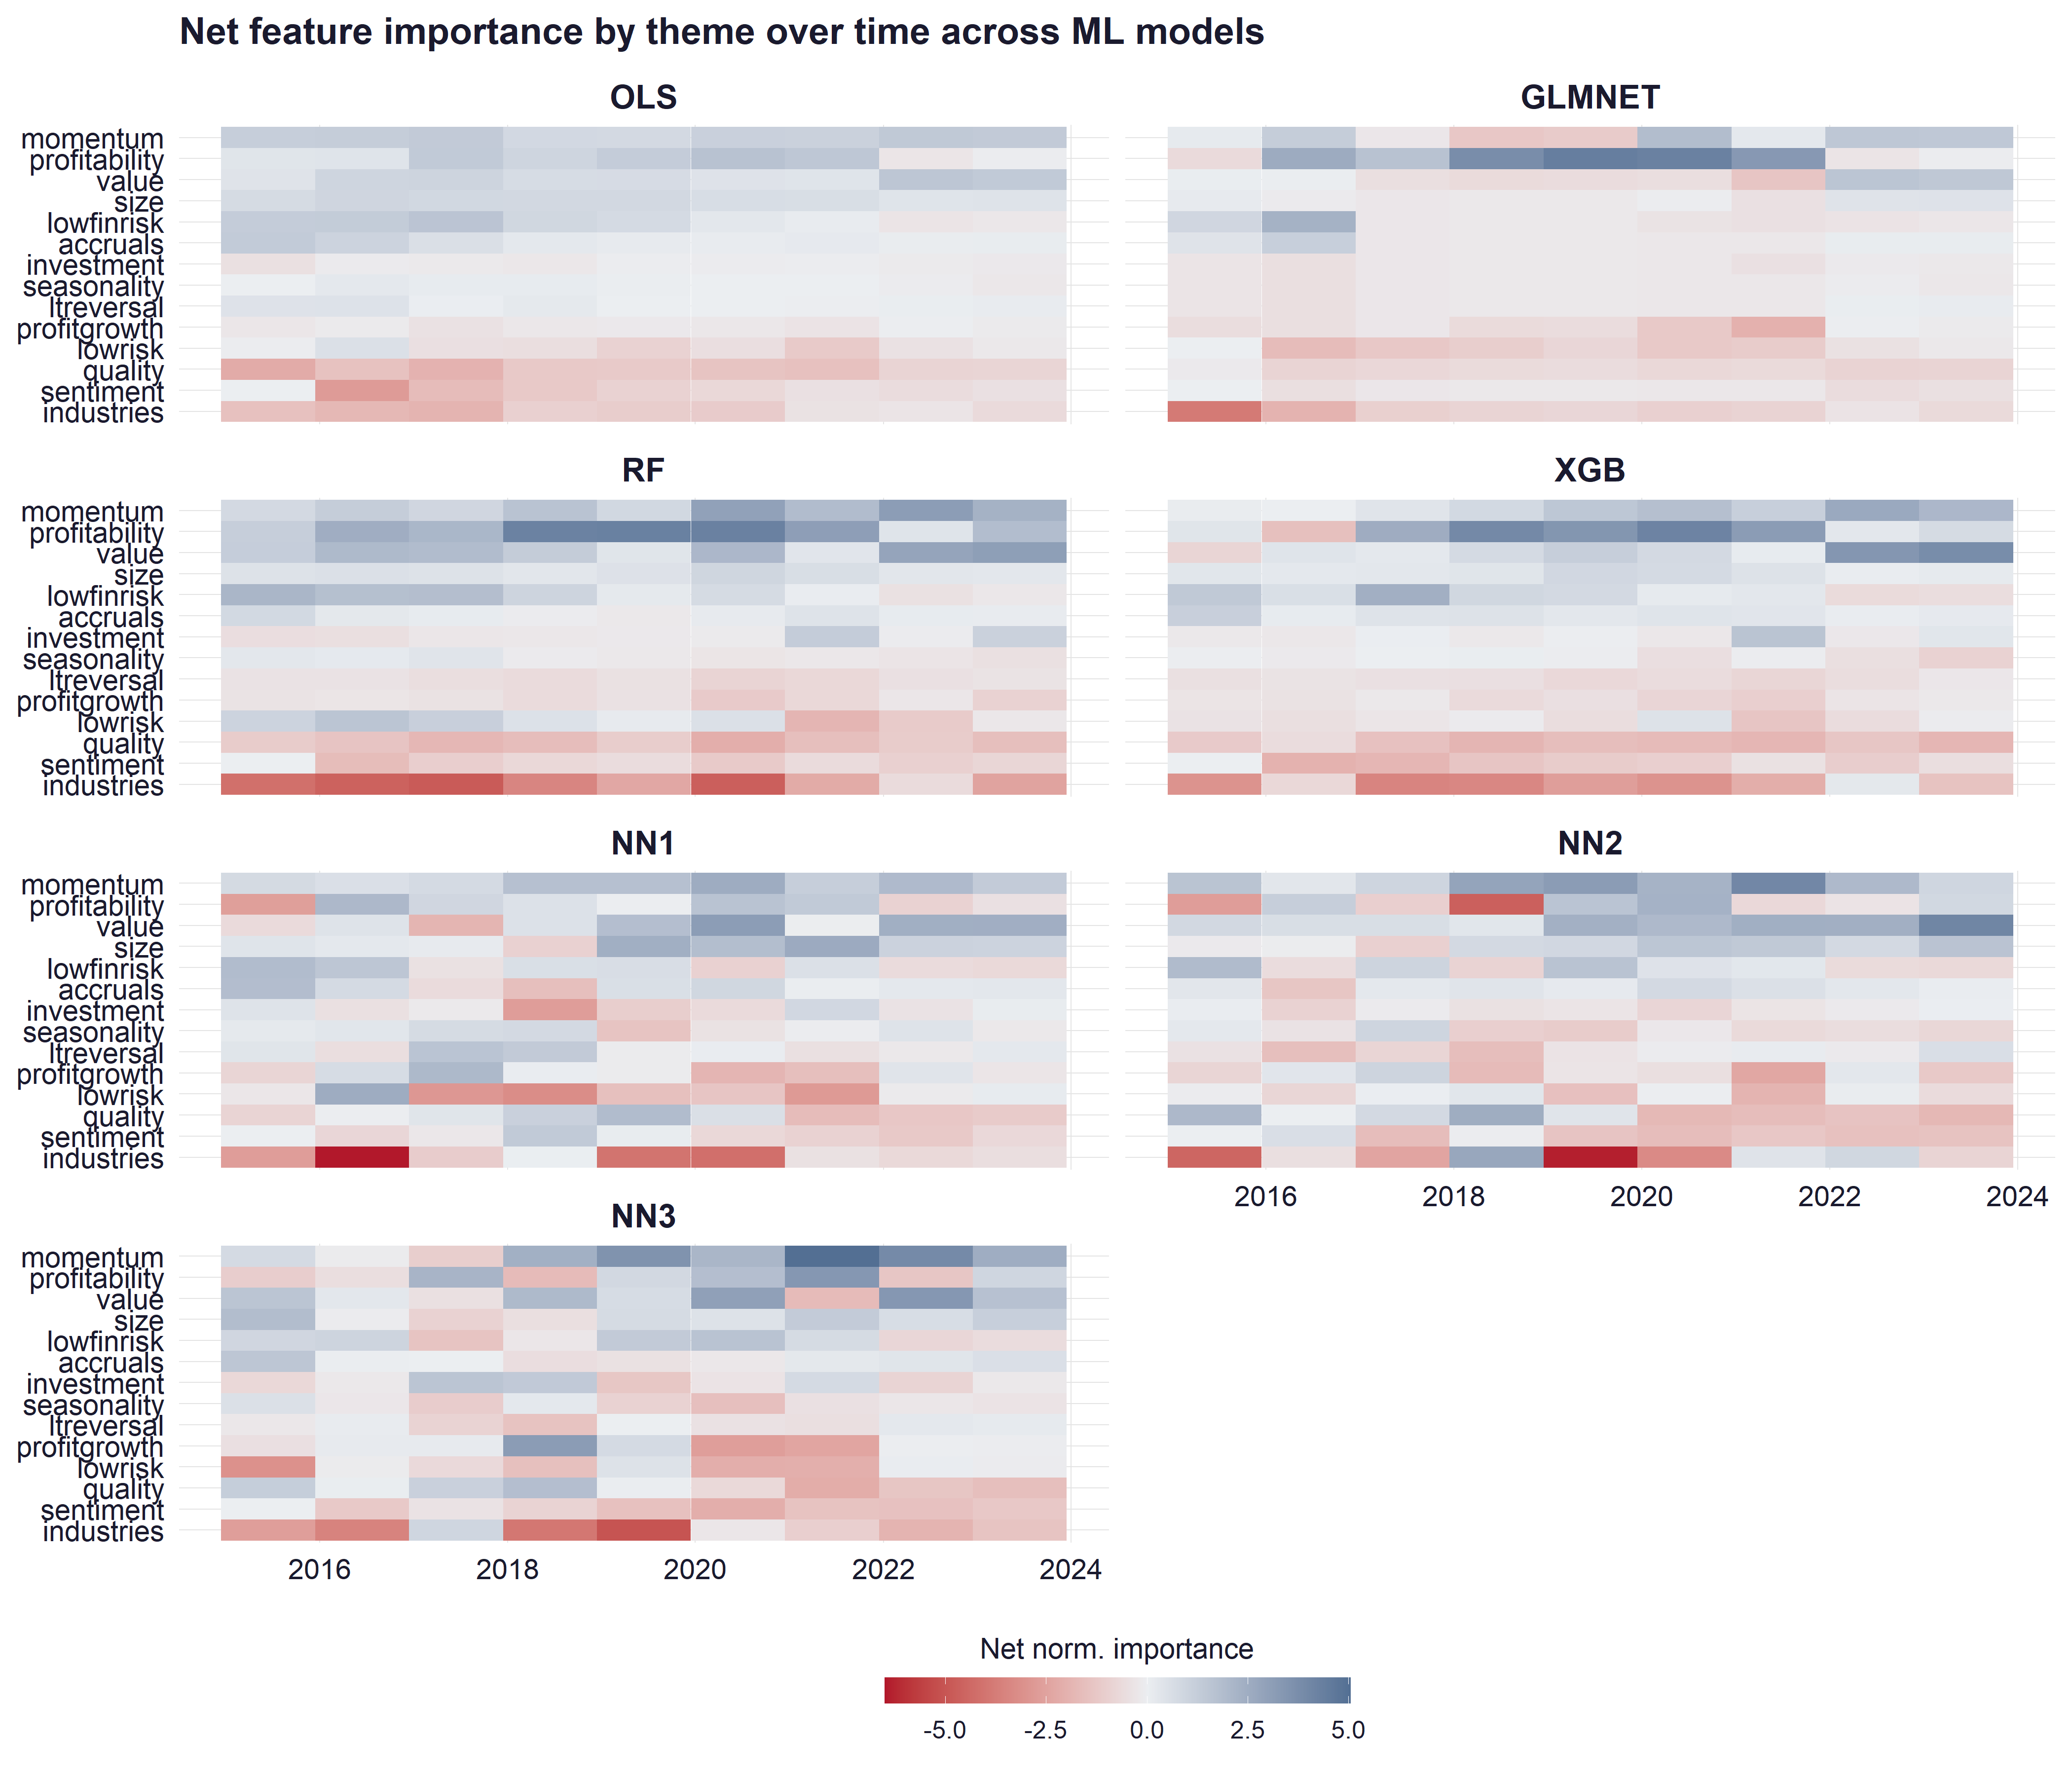
\includegraphics[width=\linewidth]{figures/feature_importance_heatmap.png}
\label{fig:fi_heatmap}
\end{figure}

\begin{figure}[htbp]
\centering
\captionsetup{
  justification=raggedright,
  labelsep=none,
  singlelinecheck=false,
  labelformat=boldlabel,
}
\caption[Gross feature importance by theme over time across ML models.]{\footnotesize \textbf{: Gross feature importance by theme over time across ML models.} Absolute surrogate loadings aggregated by characteristic theme at each refit. Theme shares sum to one within each model and refit and therefore show where coefficient mass is concentrated without allowing signs to cancel.}
\includegraphics[width=\linewidth]{figures/feature_importance_heatmap_gross.png}
\label{fig:fi_heatmap_gross}
\end{figure}


\begin{figure}[htbp]
\centering
\captionsetup{
  justification=raggedright,
  labelsep=none,
  singlelinecheck=false,
  labelformat=boldlabel,
}
\caption[Figure 7: \footnotesize ]{\footnotesize \textbf{: Linear explainability of each ML model's predictions.} For each ML model (OLS, GLMNET, RF, XGB, NN1--NN3), the out-of-sample predictions are regressed on the signals (each cross-sectionally scaled to $[-1, 1]$ that month, hence approximately mean-zero) via the OLS global surrogate model. \emph{Left (intercept):} because the scaled signals are centred, the intercept is approximately the mean of the model's predictions -- its baseline predicted active return for a characteristic-neutral (median) stock. It captures the unconditional level of predicted active returns and also absorbs any level shift induced by the model's curvature (since it equals the average prediction, $\mathrm{E}[f(x)]$, not the prediction at the average, $f(\mathrm{E}[x])$); it is a common shift across stocks and does not affect the cross-sectional ranking. \emph{Centre (}$R^2$\emph{):} the share of prediction variance that is linear in the signals -- values near one indicate an essentially linear model. \emph{Right (residual variance):} the variance of the surrogate residuals, i.e. the part of the predictions the linear surrogate cannot reproduce. Together, $1 - R^2$ and the residual variance measure the nonlinearity and interaction structure the ML model captures beyond a linear function of the signals; both are near zero for the linear models (OLS, GLMNET) and larger for the tree and neural-network models. Values are for the final-refit surrogate on the individual-signals run.}
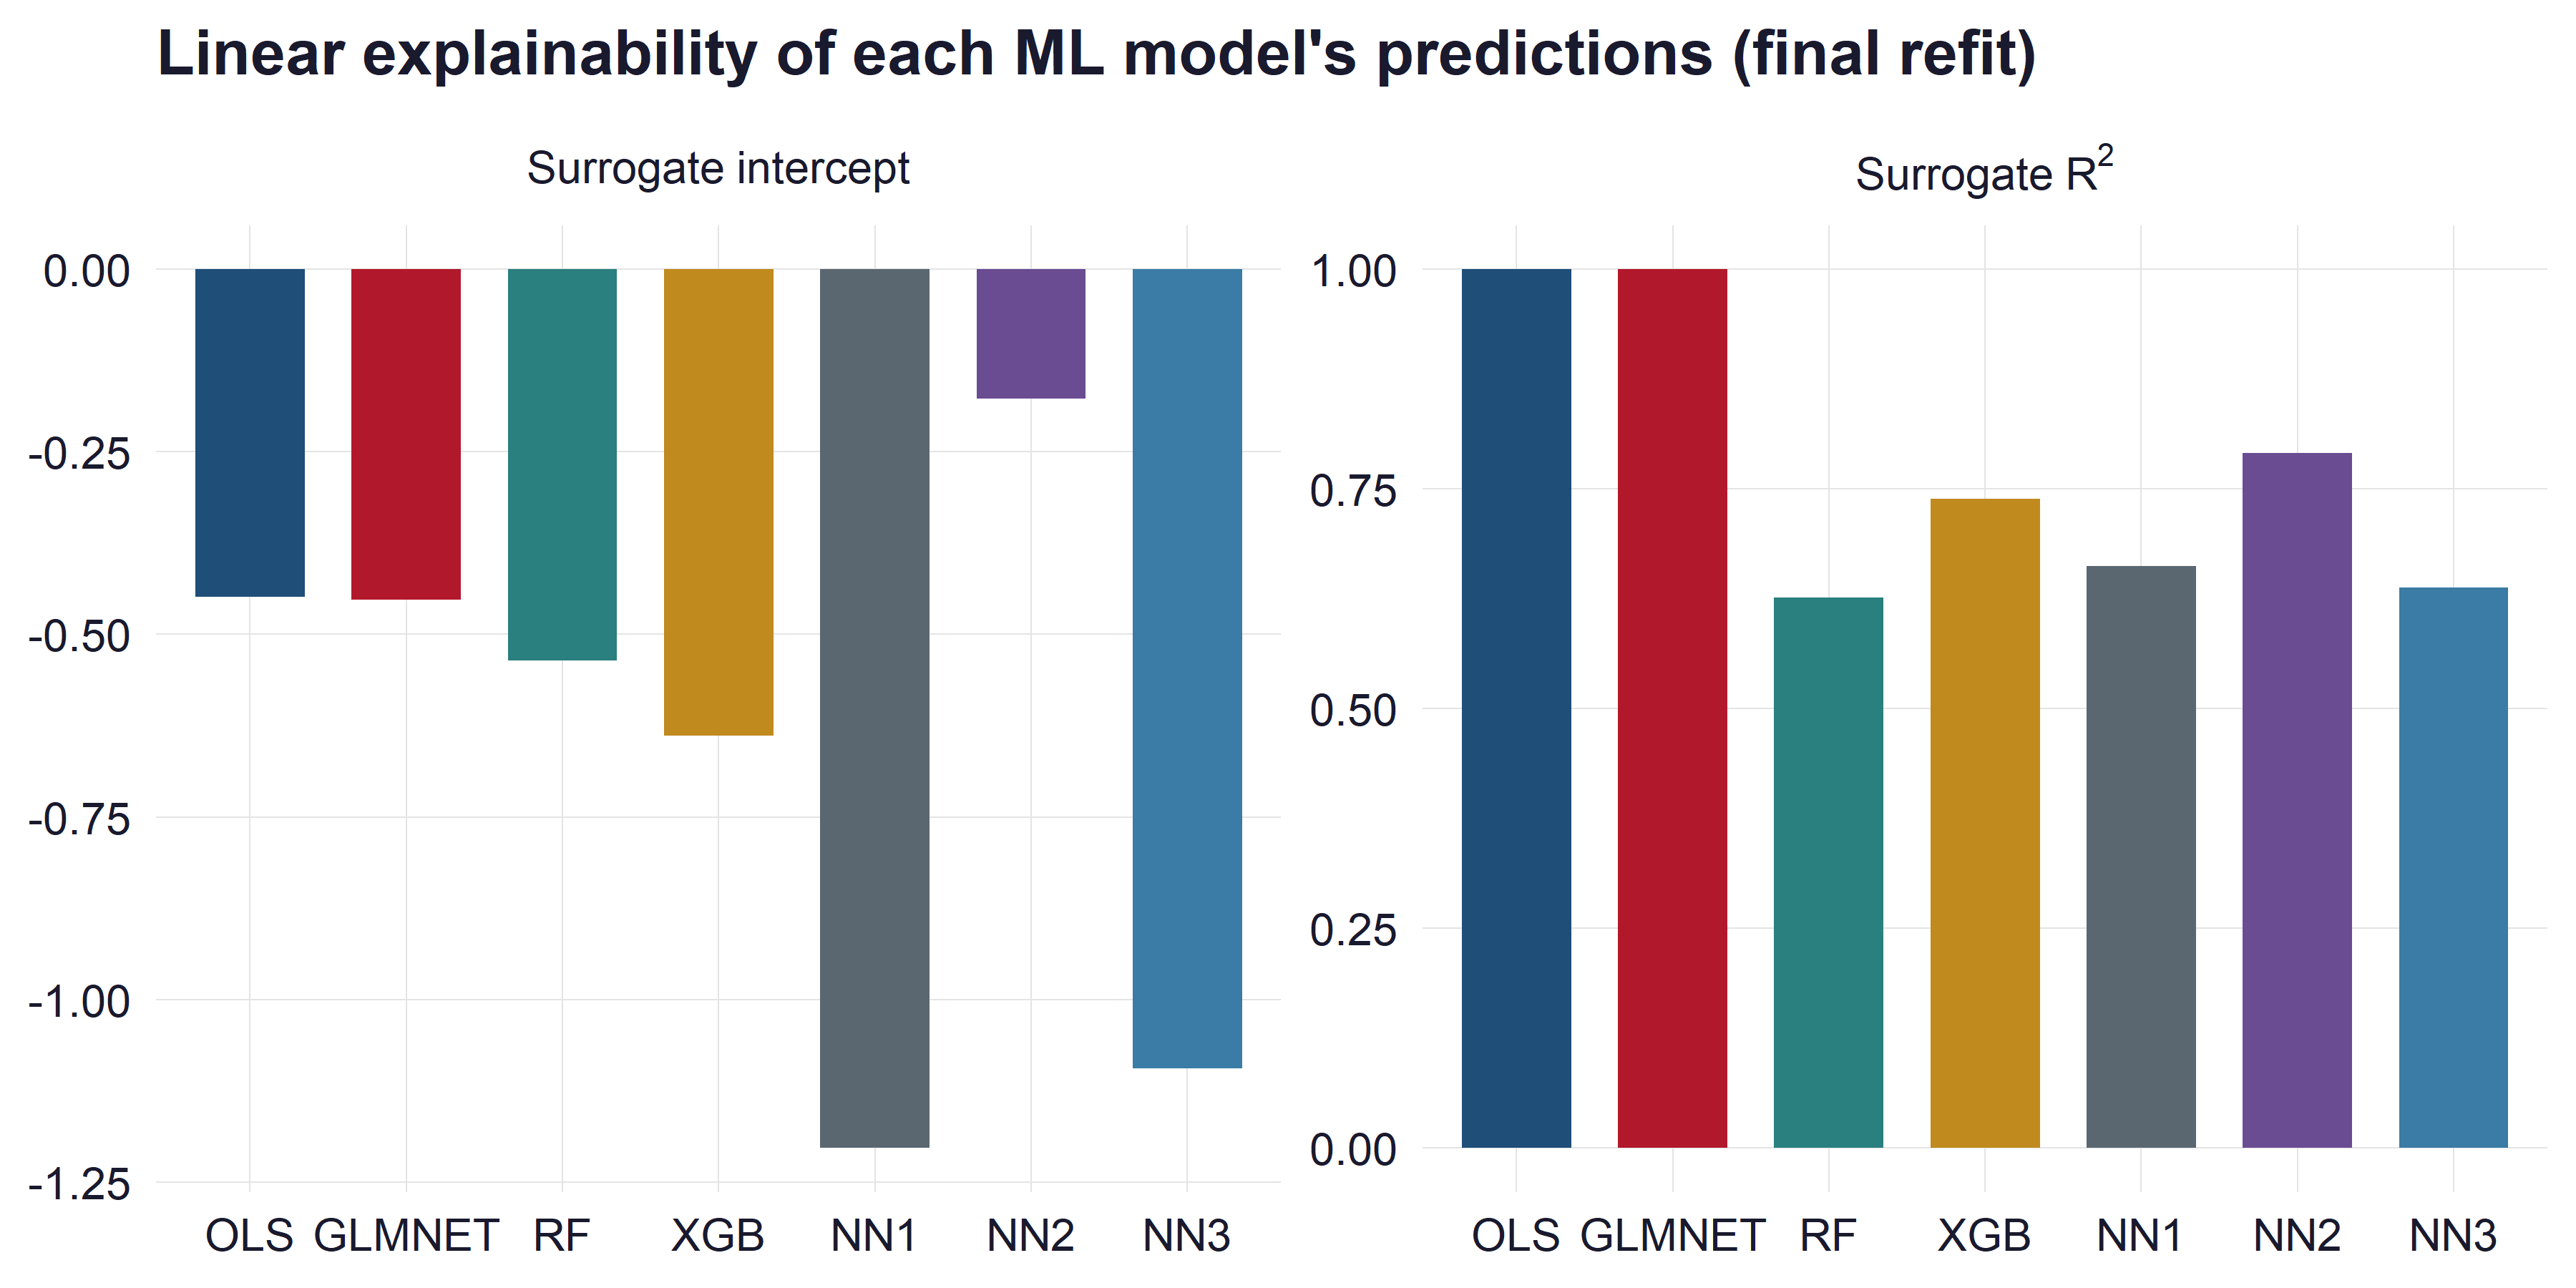
\includegraphics[width=\linewidth]{figures/surrogate_fit.png}
\label{fig:surrogate_fit}
\end{figure}


\begin{figure}[htbp]
\centering
\captionsetup{
  justification=raggedright,
  labelsep=none,
  singlelinecheck=false,
  labelformat=boldlabel,
}
\caption[Figure 3: \footnotesize ]{\footnotesize \textbf{: Portfolio weight composition by sector.} Out-of-sample monthly composition of portfolio weight across economic sectors, for each ML-ensemble portfolio-construction scheme (RP, RP\_BOX, HRP, CS, SW, EW, MVO, MVO\_BOX) and the IBOV benchmark. Each panel stacks the sum of portfolio weights within each sector to 100\% at every rebalance date.}
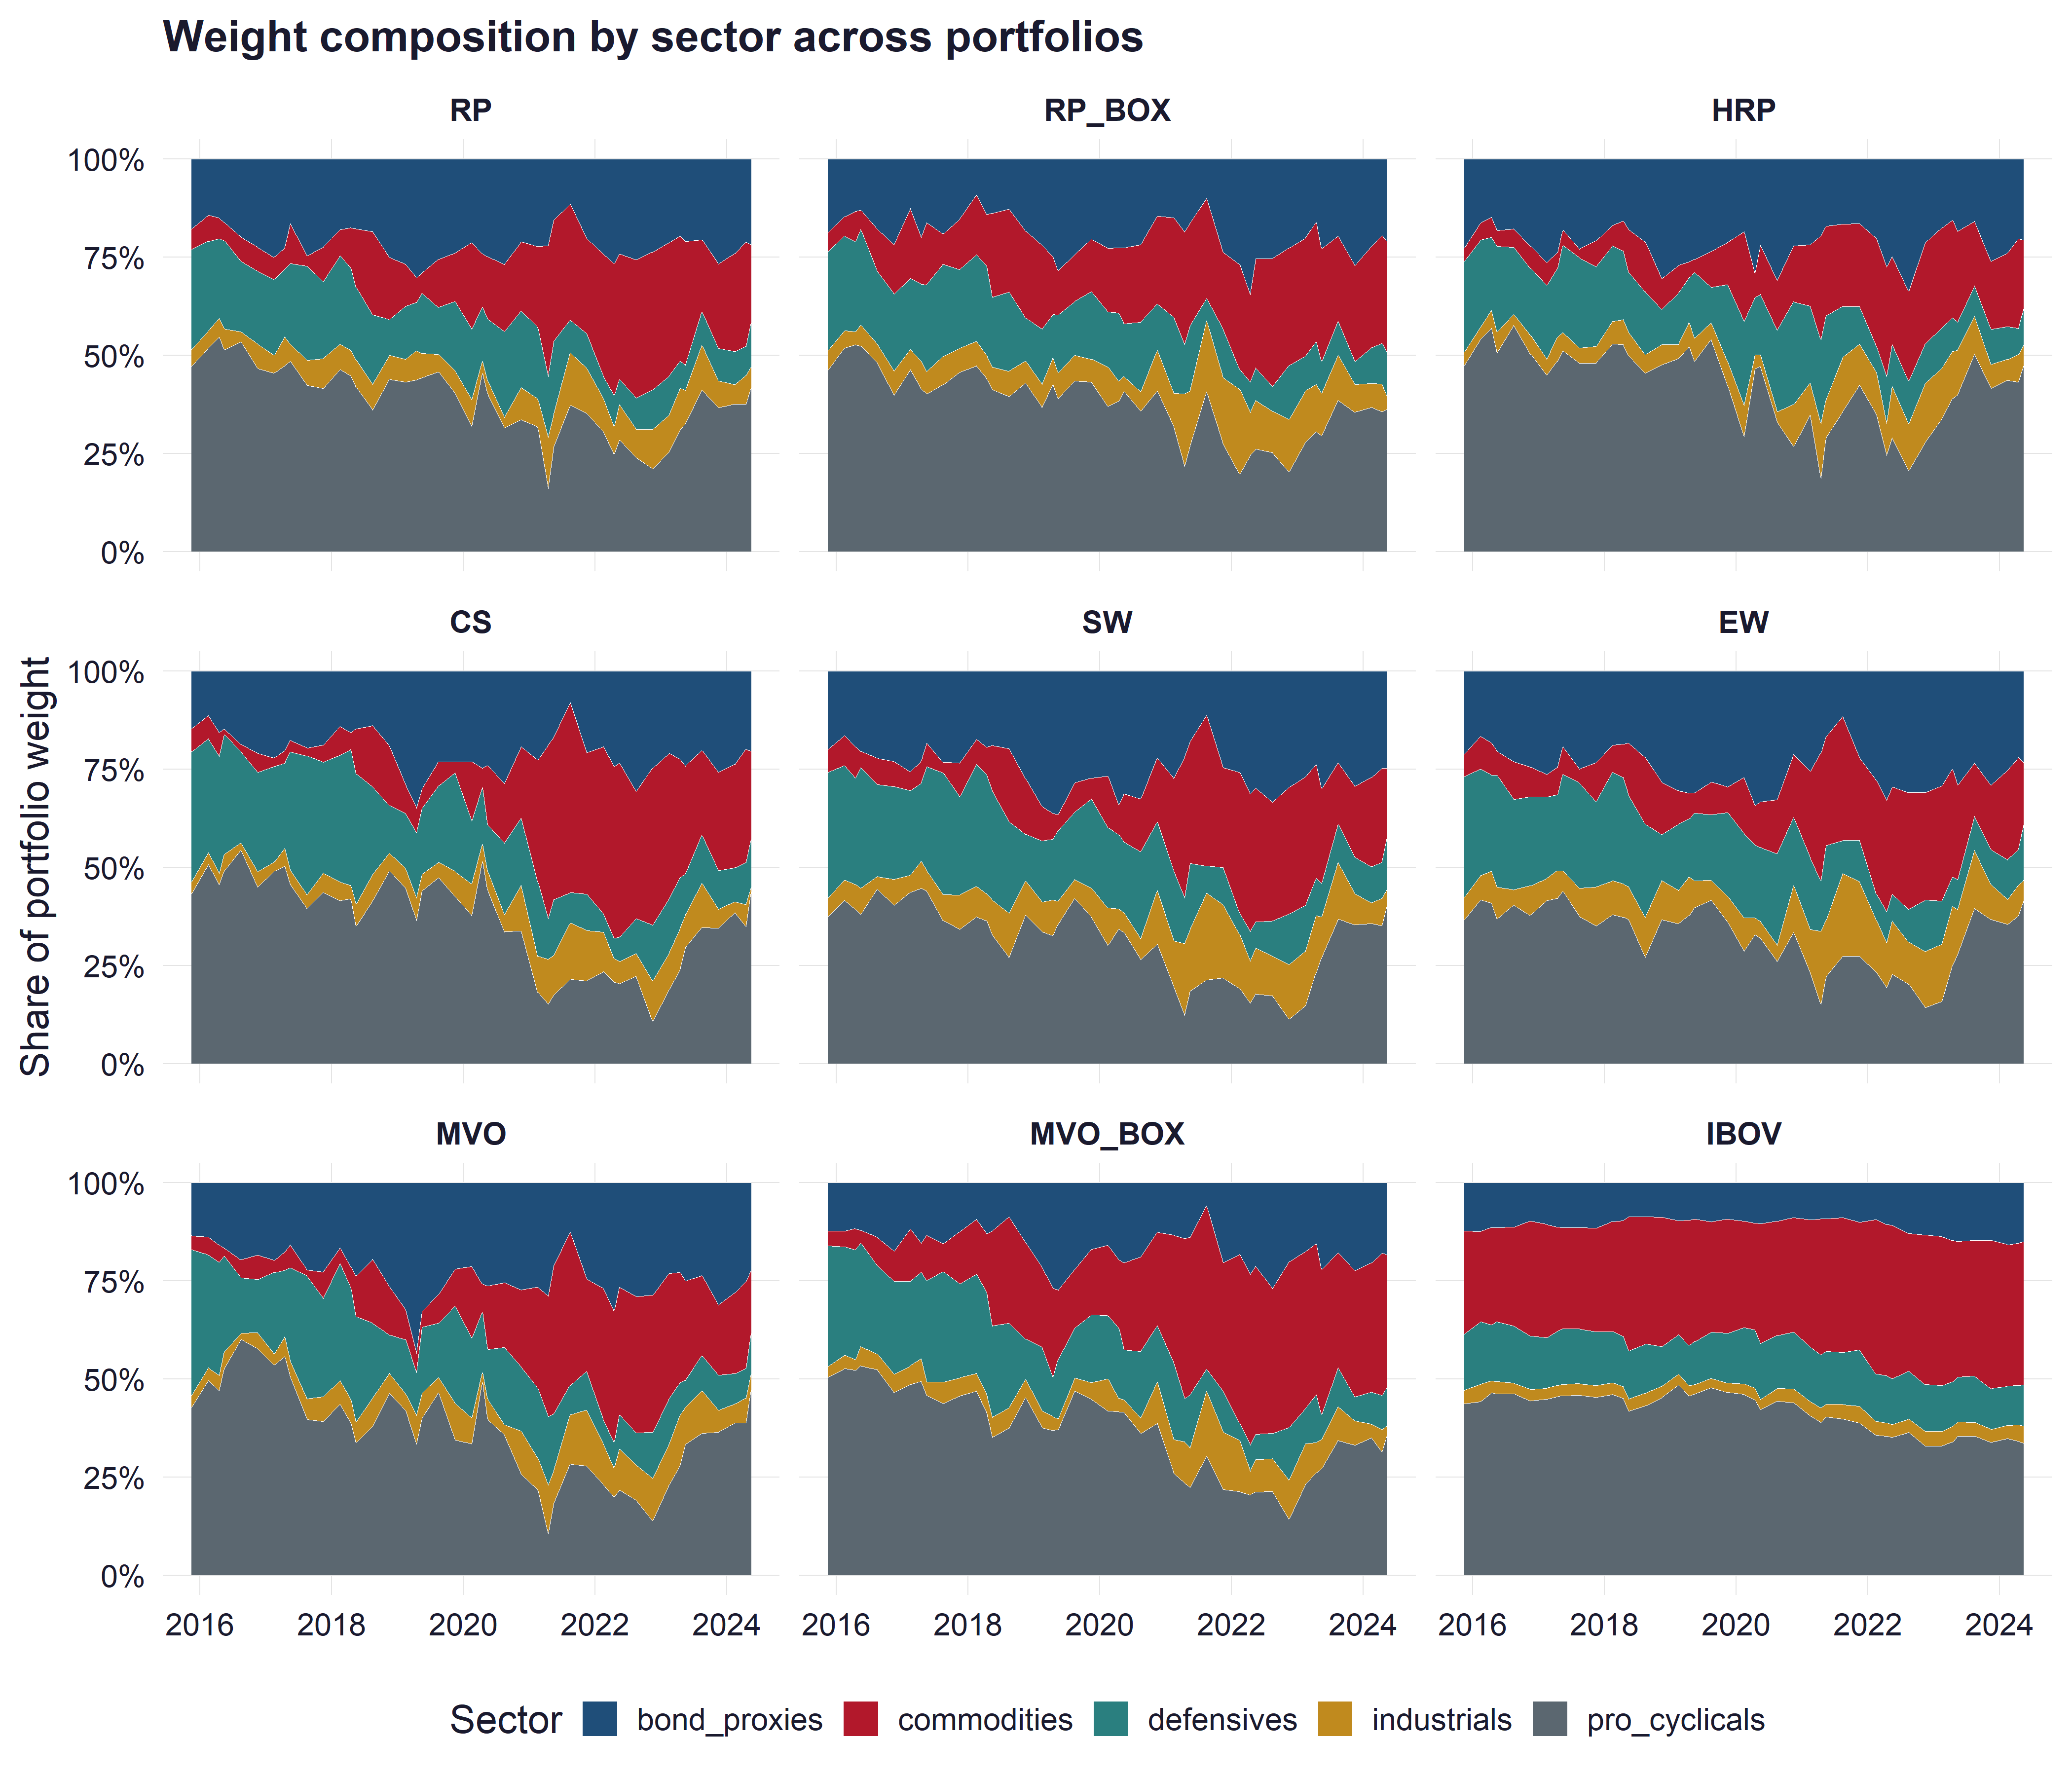
\includegraphics[width=\linewidth]{figures/composition_sector_weight.png}
\label{fig:comp_sector}
\end{figure}

\begin{figure}[htbp]
\centering
\captionsetup{
  justification=raggedright,
  labelsep=none,
  singlelinecheck=false,
  labelformat=boldlabel,
}
\caption[Figure 4: \footnotesize ]{\footnotesize \textbf{: Portfolio weight composition by market capitalization.} Out-of-sample monthly composition of portfolio weight across market-capitalization classes (mega, large, mid, small and micro caps), for each ML-ensemble portfolio-construction scheme and the IBOV benchmark. Each panel stacks the sum of portfolio weights within each size class to 100\% at every rebalance date.}
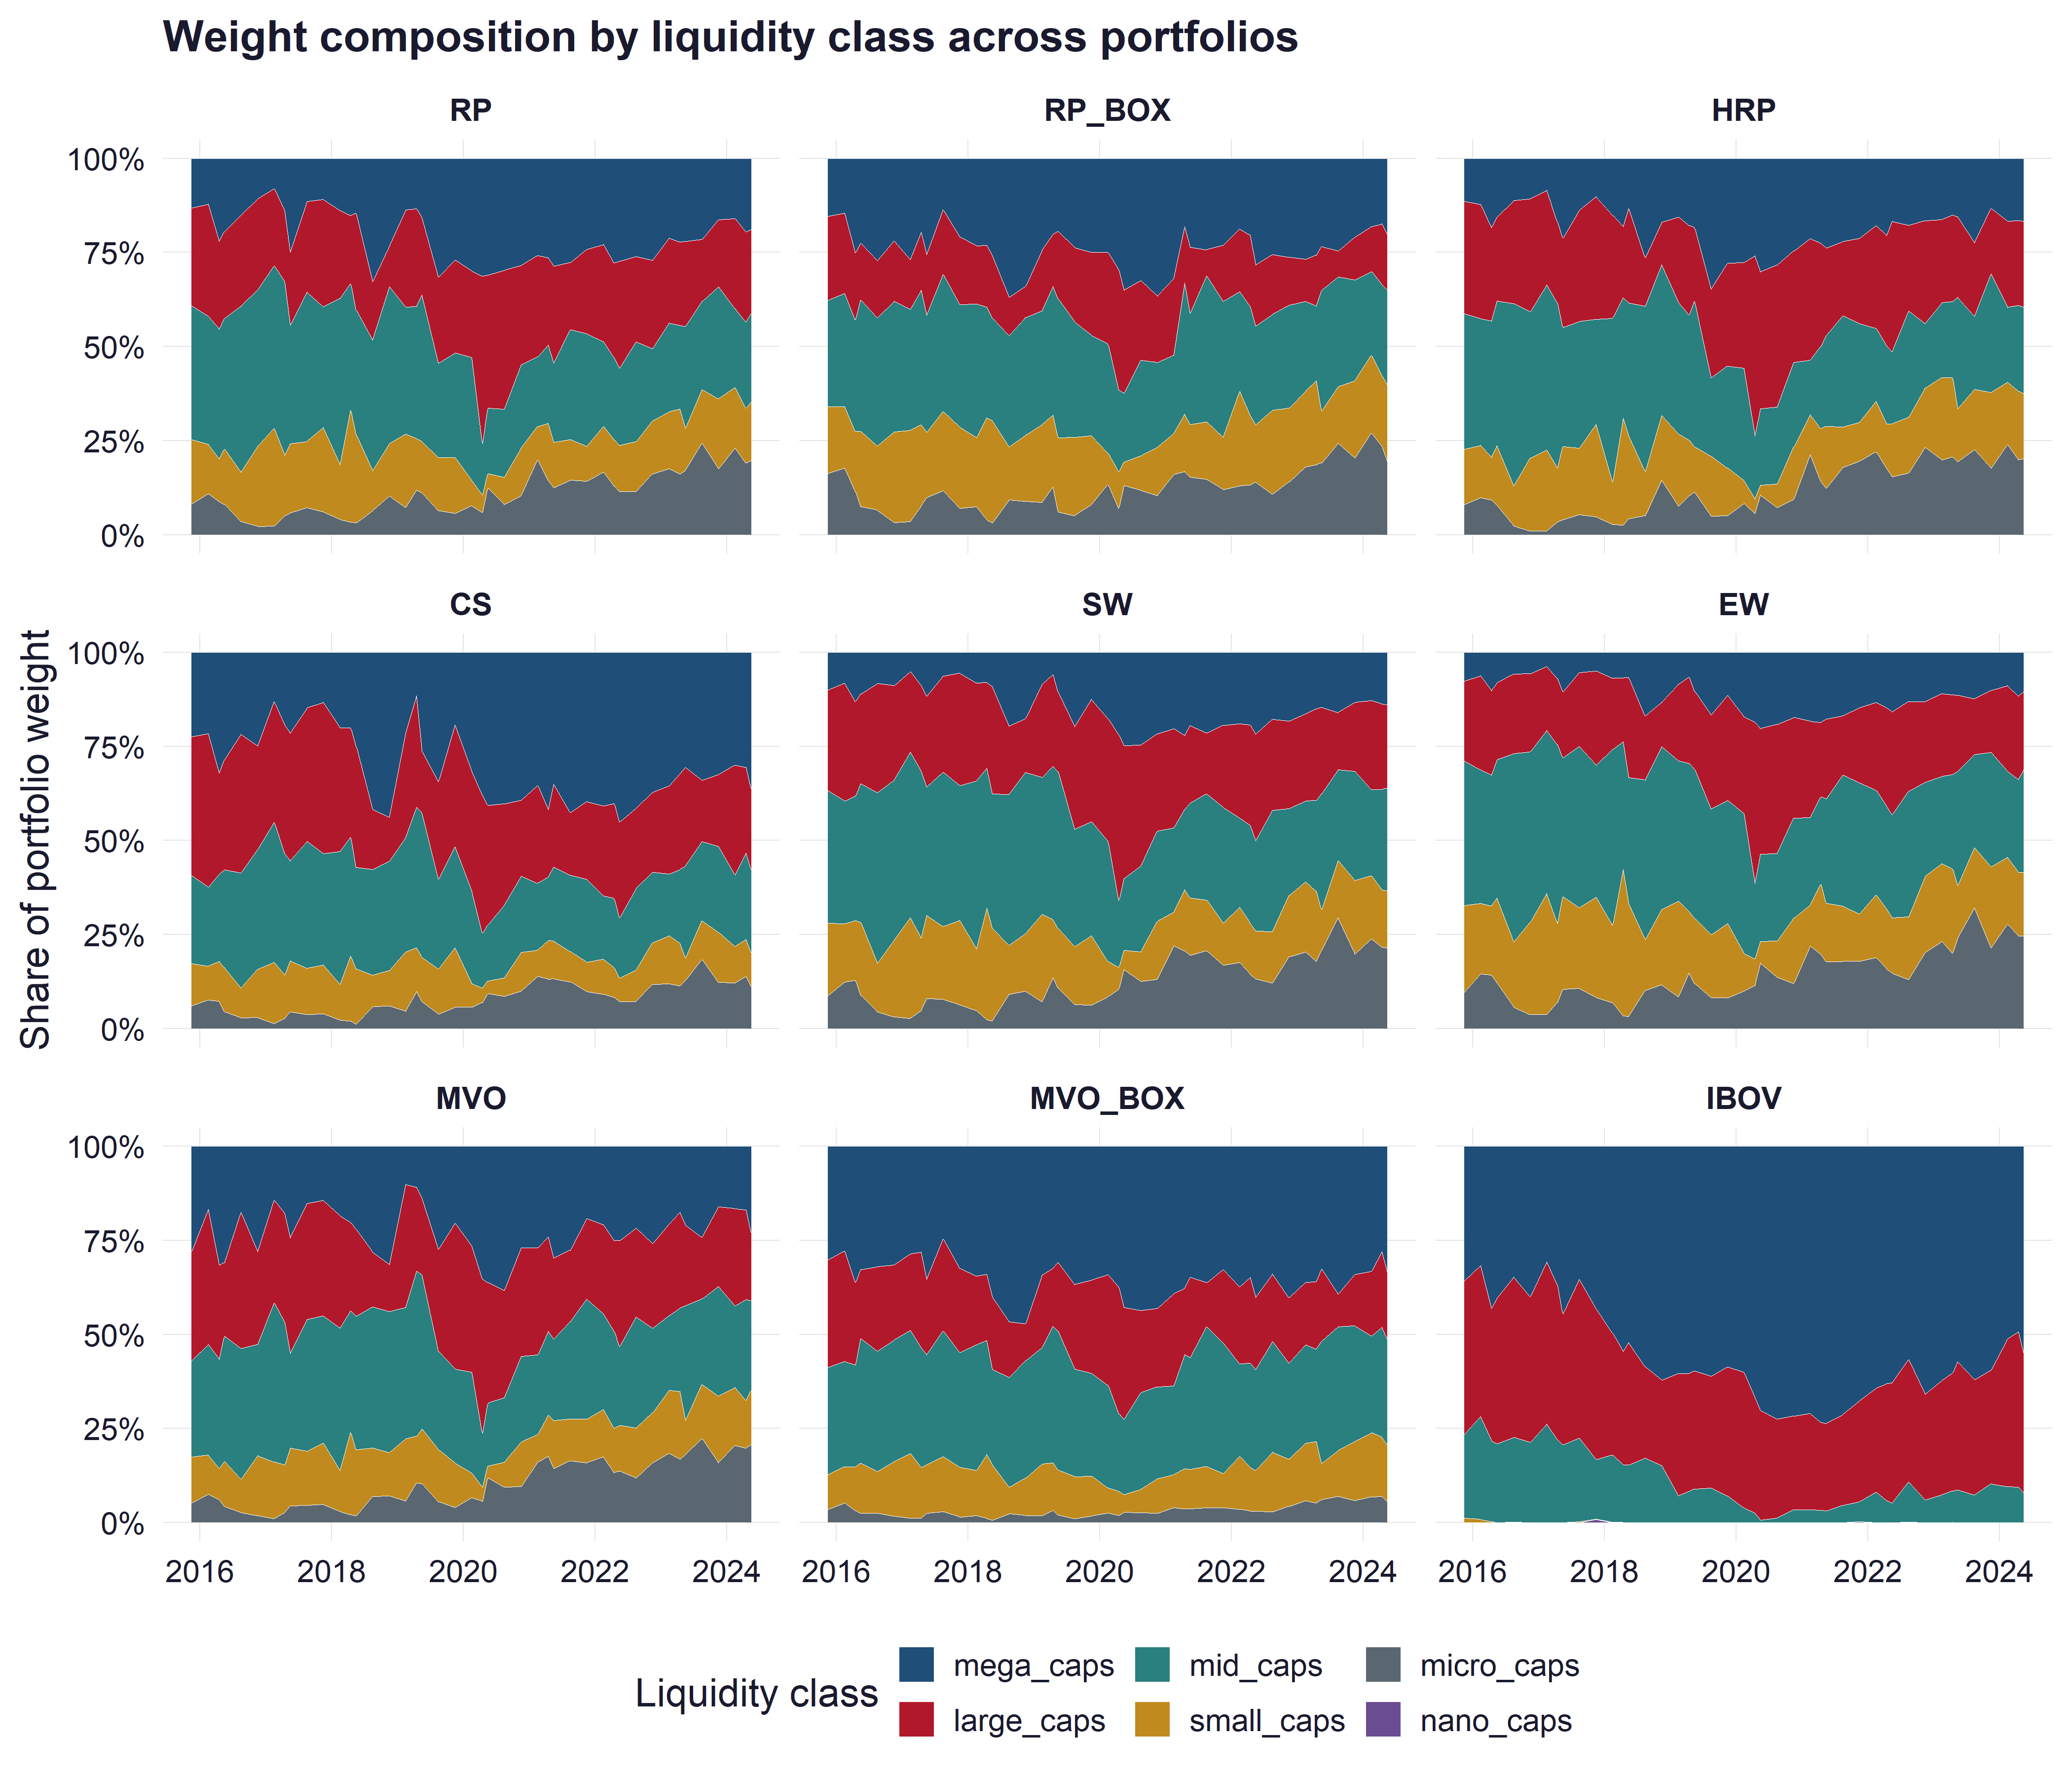
\includegraphics[width=\linewidth]{figures/composition_liquidity_weight.png}
\label{fig:comp_mktcap}
\end{figure}


\begin{figure}[htbp]
\centering
\captionsetup{
  justification=raggedright,
  labelsep=none,
  singlelinecheck=false,
  labelformat=boldlabel,
}
\caption[Figure 10: \footnotesize ]{\footnotesize \textbf{: Agreement across base-learner predictions.} Pairwise correlation of the out-of-sample return predictions of the seven base learners (OLS, GLMNET, RF, XGB, NN1--NN3). Correlations are computed cross-sectionally within each month and then averaged over months, so they measure whether the models rank the same stocks alike rather than sharing a common time-series level. Lower correlations indicate more independent signals and hence more scope for the ensemble to add value.}
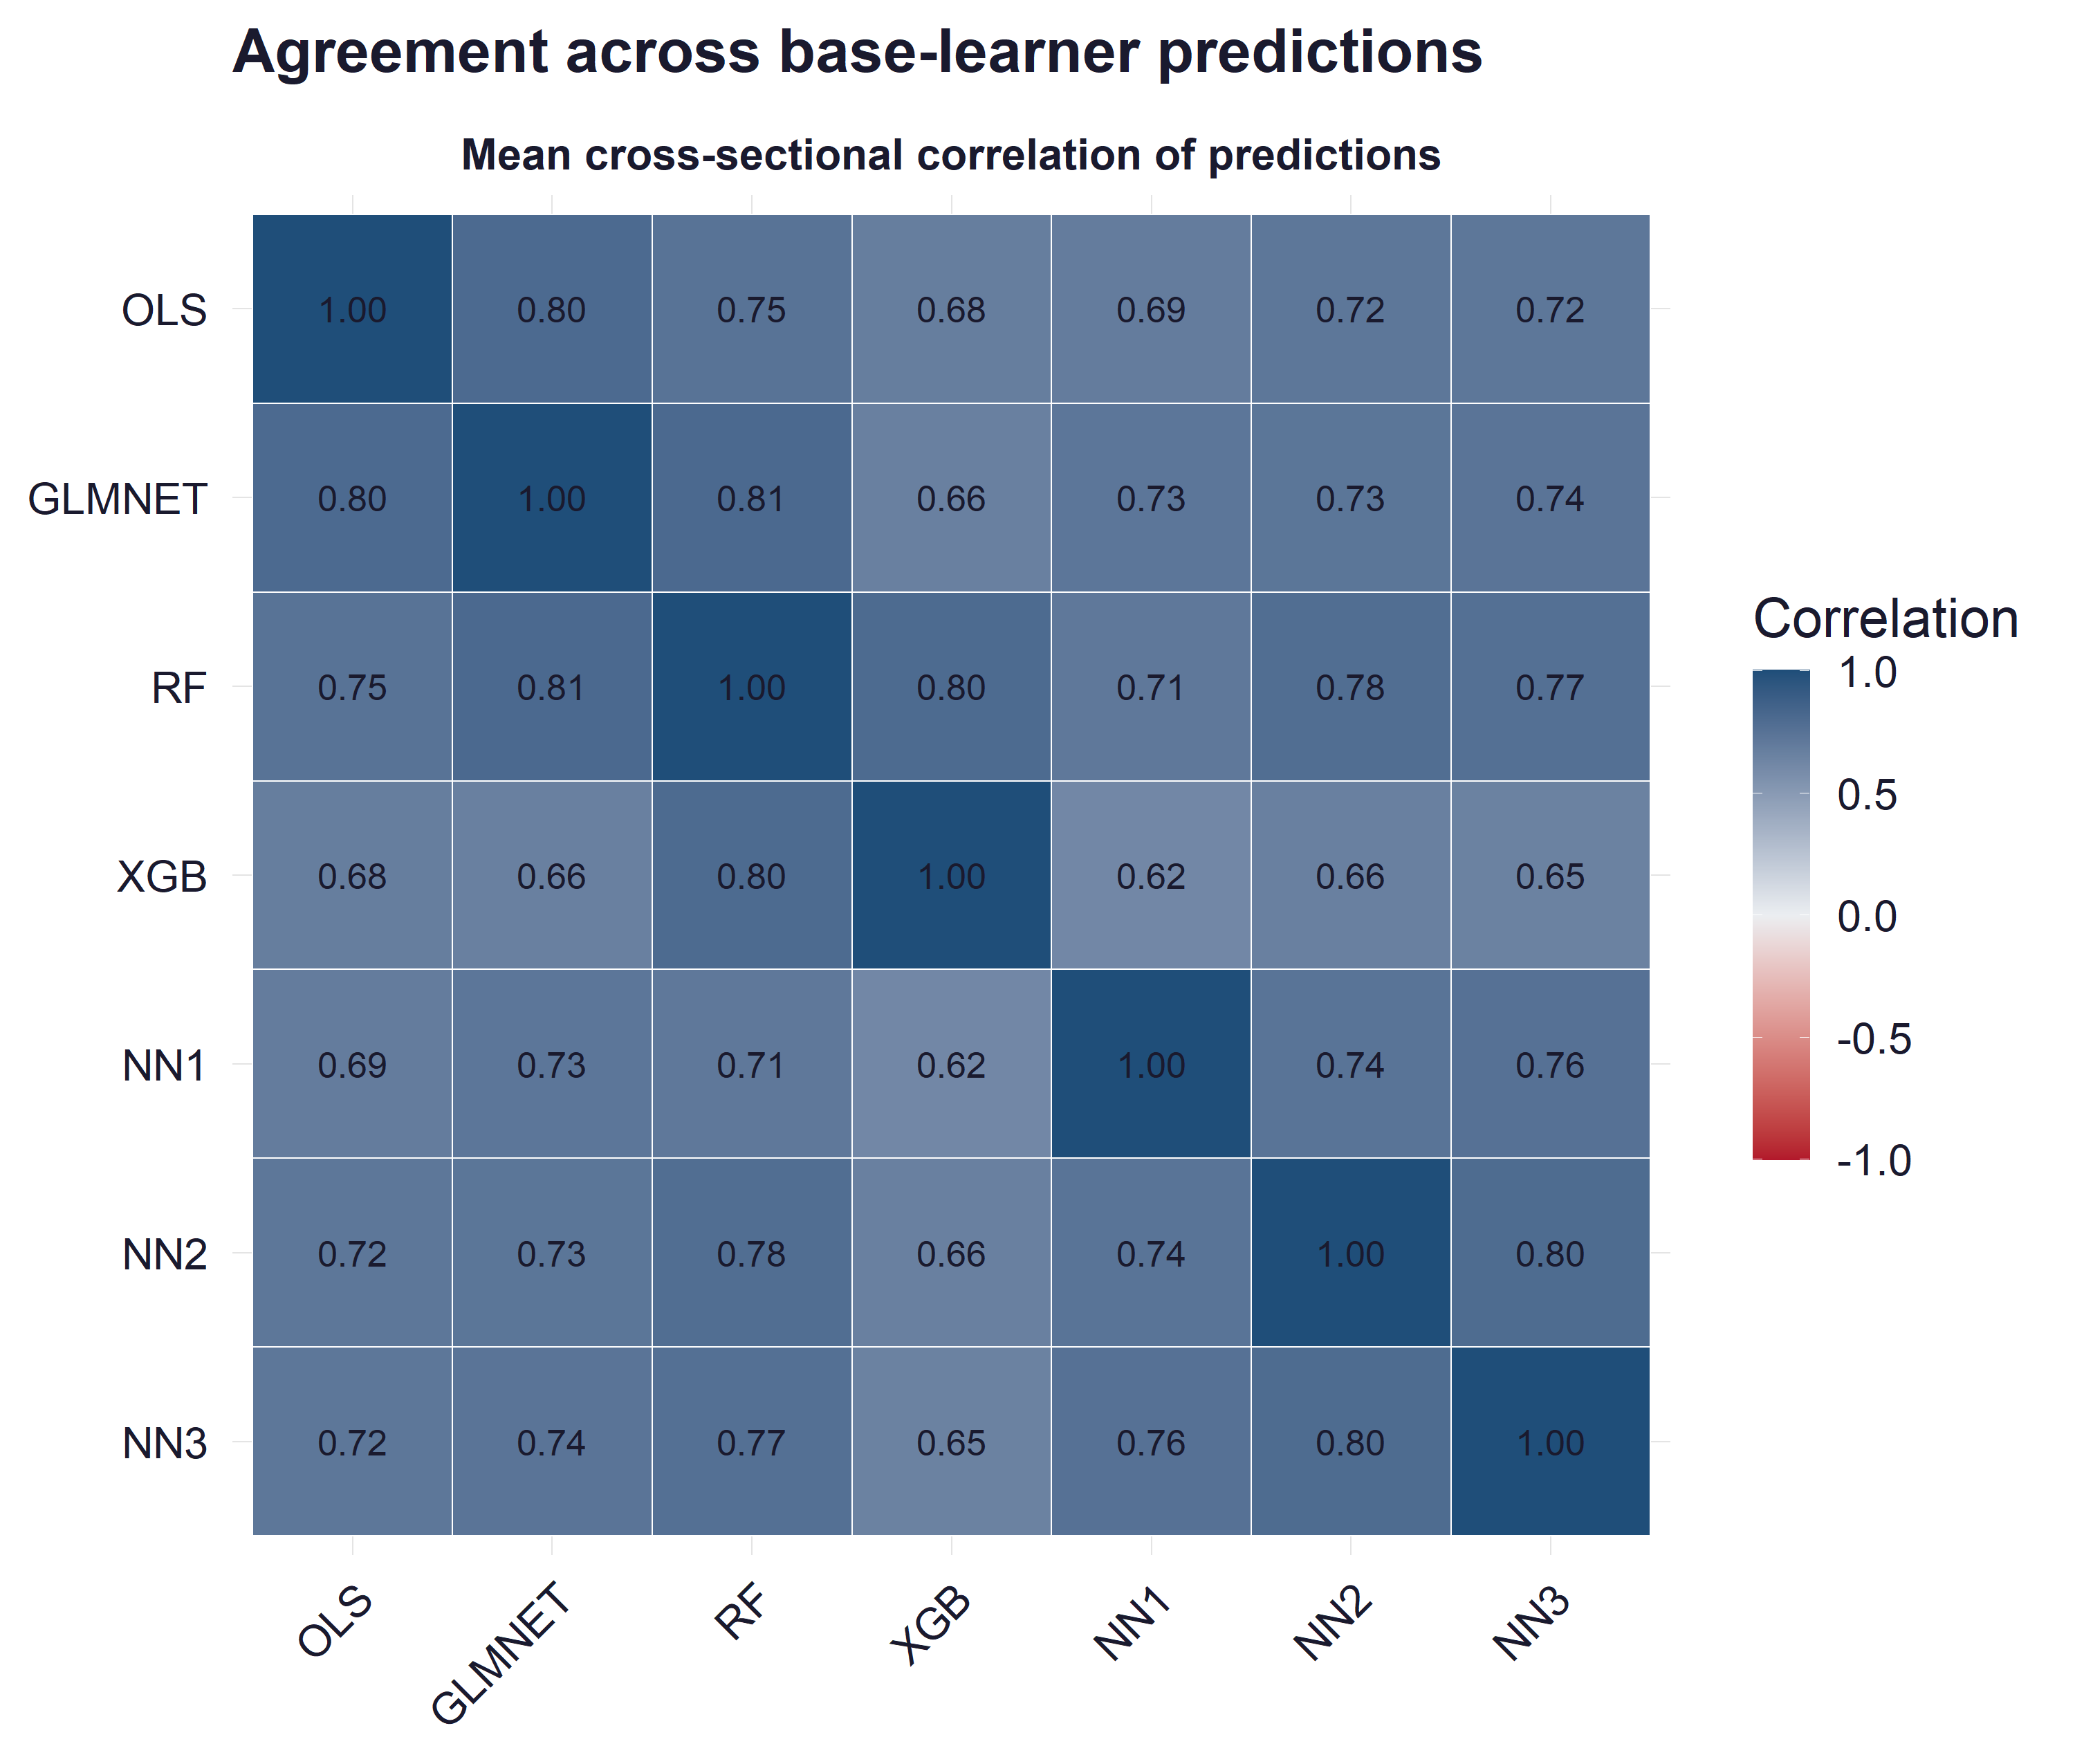
\includegraphics[width=\linewidth]{figures/correlogram_predictions.png}
\label{fig:corr_pred}
\end{figure}

\begin{figure}[htbp]
\centering
\captionsetup{
  justification=raggedright,
  labelsep=none,
  singlelinecheck=false,
  labelformat=boldlabel,
}
\caption[Figure 11: \footnotesize ]{\footnotesize \textbf{: Active return correlation: ML Ensemble portfolios vs human managers.} Monthly active return correlations (each series measured net of IBOV) among the eight ML Ensemble portfolio-construction schemes and the human-manager benchmarks FUNDS\_MEAN and FUNDS\_Q75. Active rather than raw returns are shown because the common market exposure of long-only portfolios mechanically pushes every raw-return pair toward one. All fund and IBOV returns are geometrically compounded 15th-to-15th to match the ML backtest. AVG\_FUND and AVG\_FUND\_Q75 are not return series: their entries average each portfolio's correlations with, respectively, all reliable funds and reliable top-quartile funds. Their diagonal entries average distinct within-cohort fund pairs and therefore are not equal to one. Lower ML-versus-fund correlations indicate greater diversification potential from combining machine and human portfolios.}
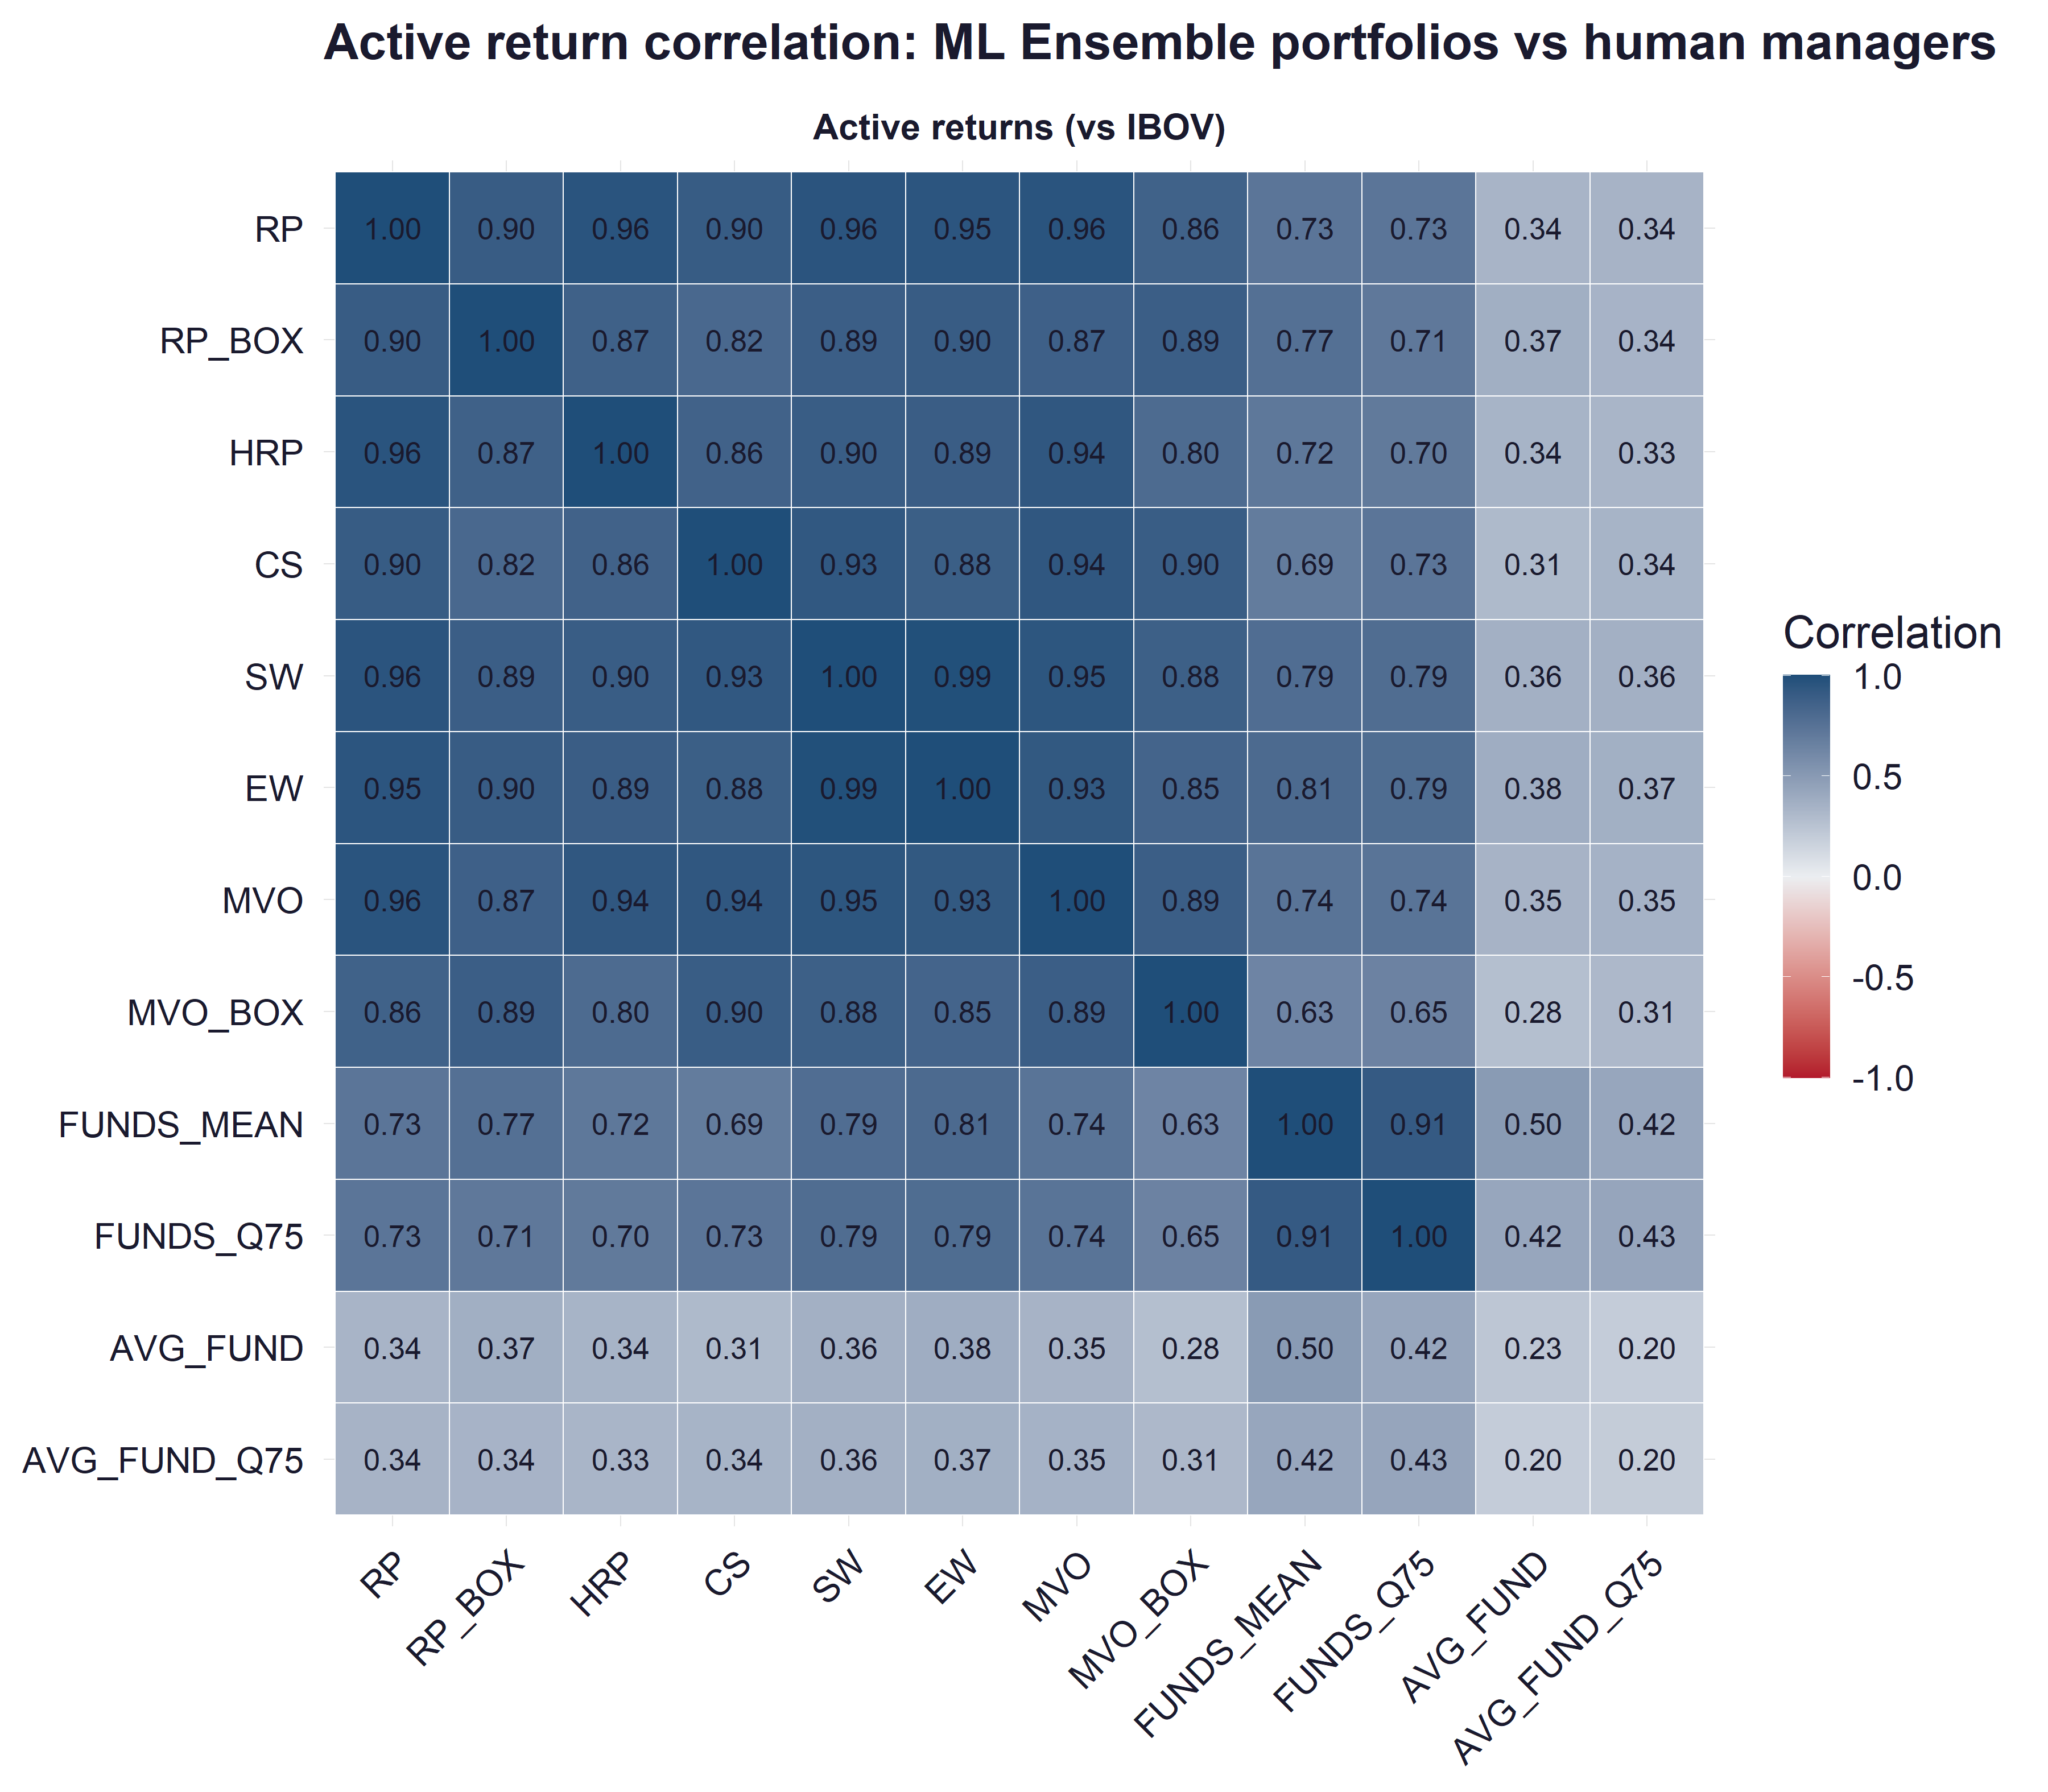
\includegraphics[width=\linewidth]{figures/correlogram_performance.png}
\label{fig:corr_perf}
\end{figure}


\begin{figure}[htbp]
\centering
\captionsetup{
  justification=raggedright,
  labelsep=none,
  singlelinecheck=false,
  labelformat=boldlabel,
}
\caption[Figure 13: \footnotesize ]{\footnotesize \textbf{: Fund-picking sensitivity of the combination frontier.} Funds are ranked by their full-window 15th-to-15th geometric return, and the retained share varies from the top 50\% to the top 5\%. Red lines show the Information Ratio of the equal-weight human portfolio; blue lines show the maximum Information Ratio over five-percentage-point combinations with each ML portfolio. RP is highlighted because it is the pre-specified transparent, risk-controlled ensemble, not because it is ex-post best; the other seven ML schemes show whether the quantile pattern generalizes. The dotted line marks the baseline top quartile. In the RP panel, shading is the 95\% interval from 999 joint circular 12-month block-bootstrap samples with funds re-ranked in each sample. Because the main rankings use the full window, these curves are oracle sensitivity bounds rather than implementable investment strategies.}
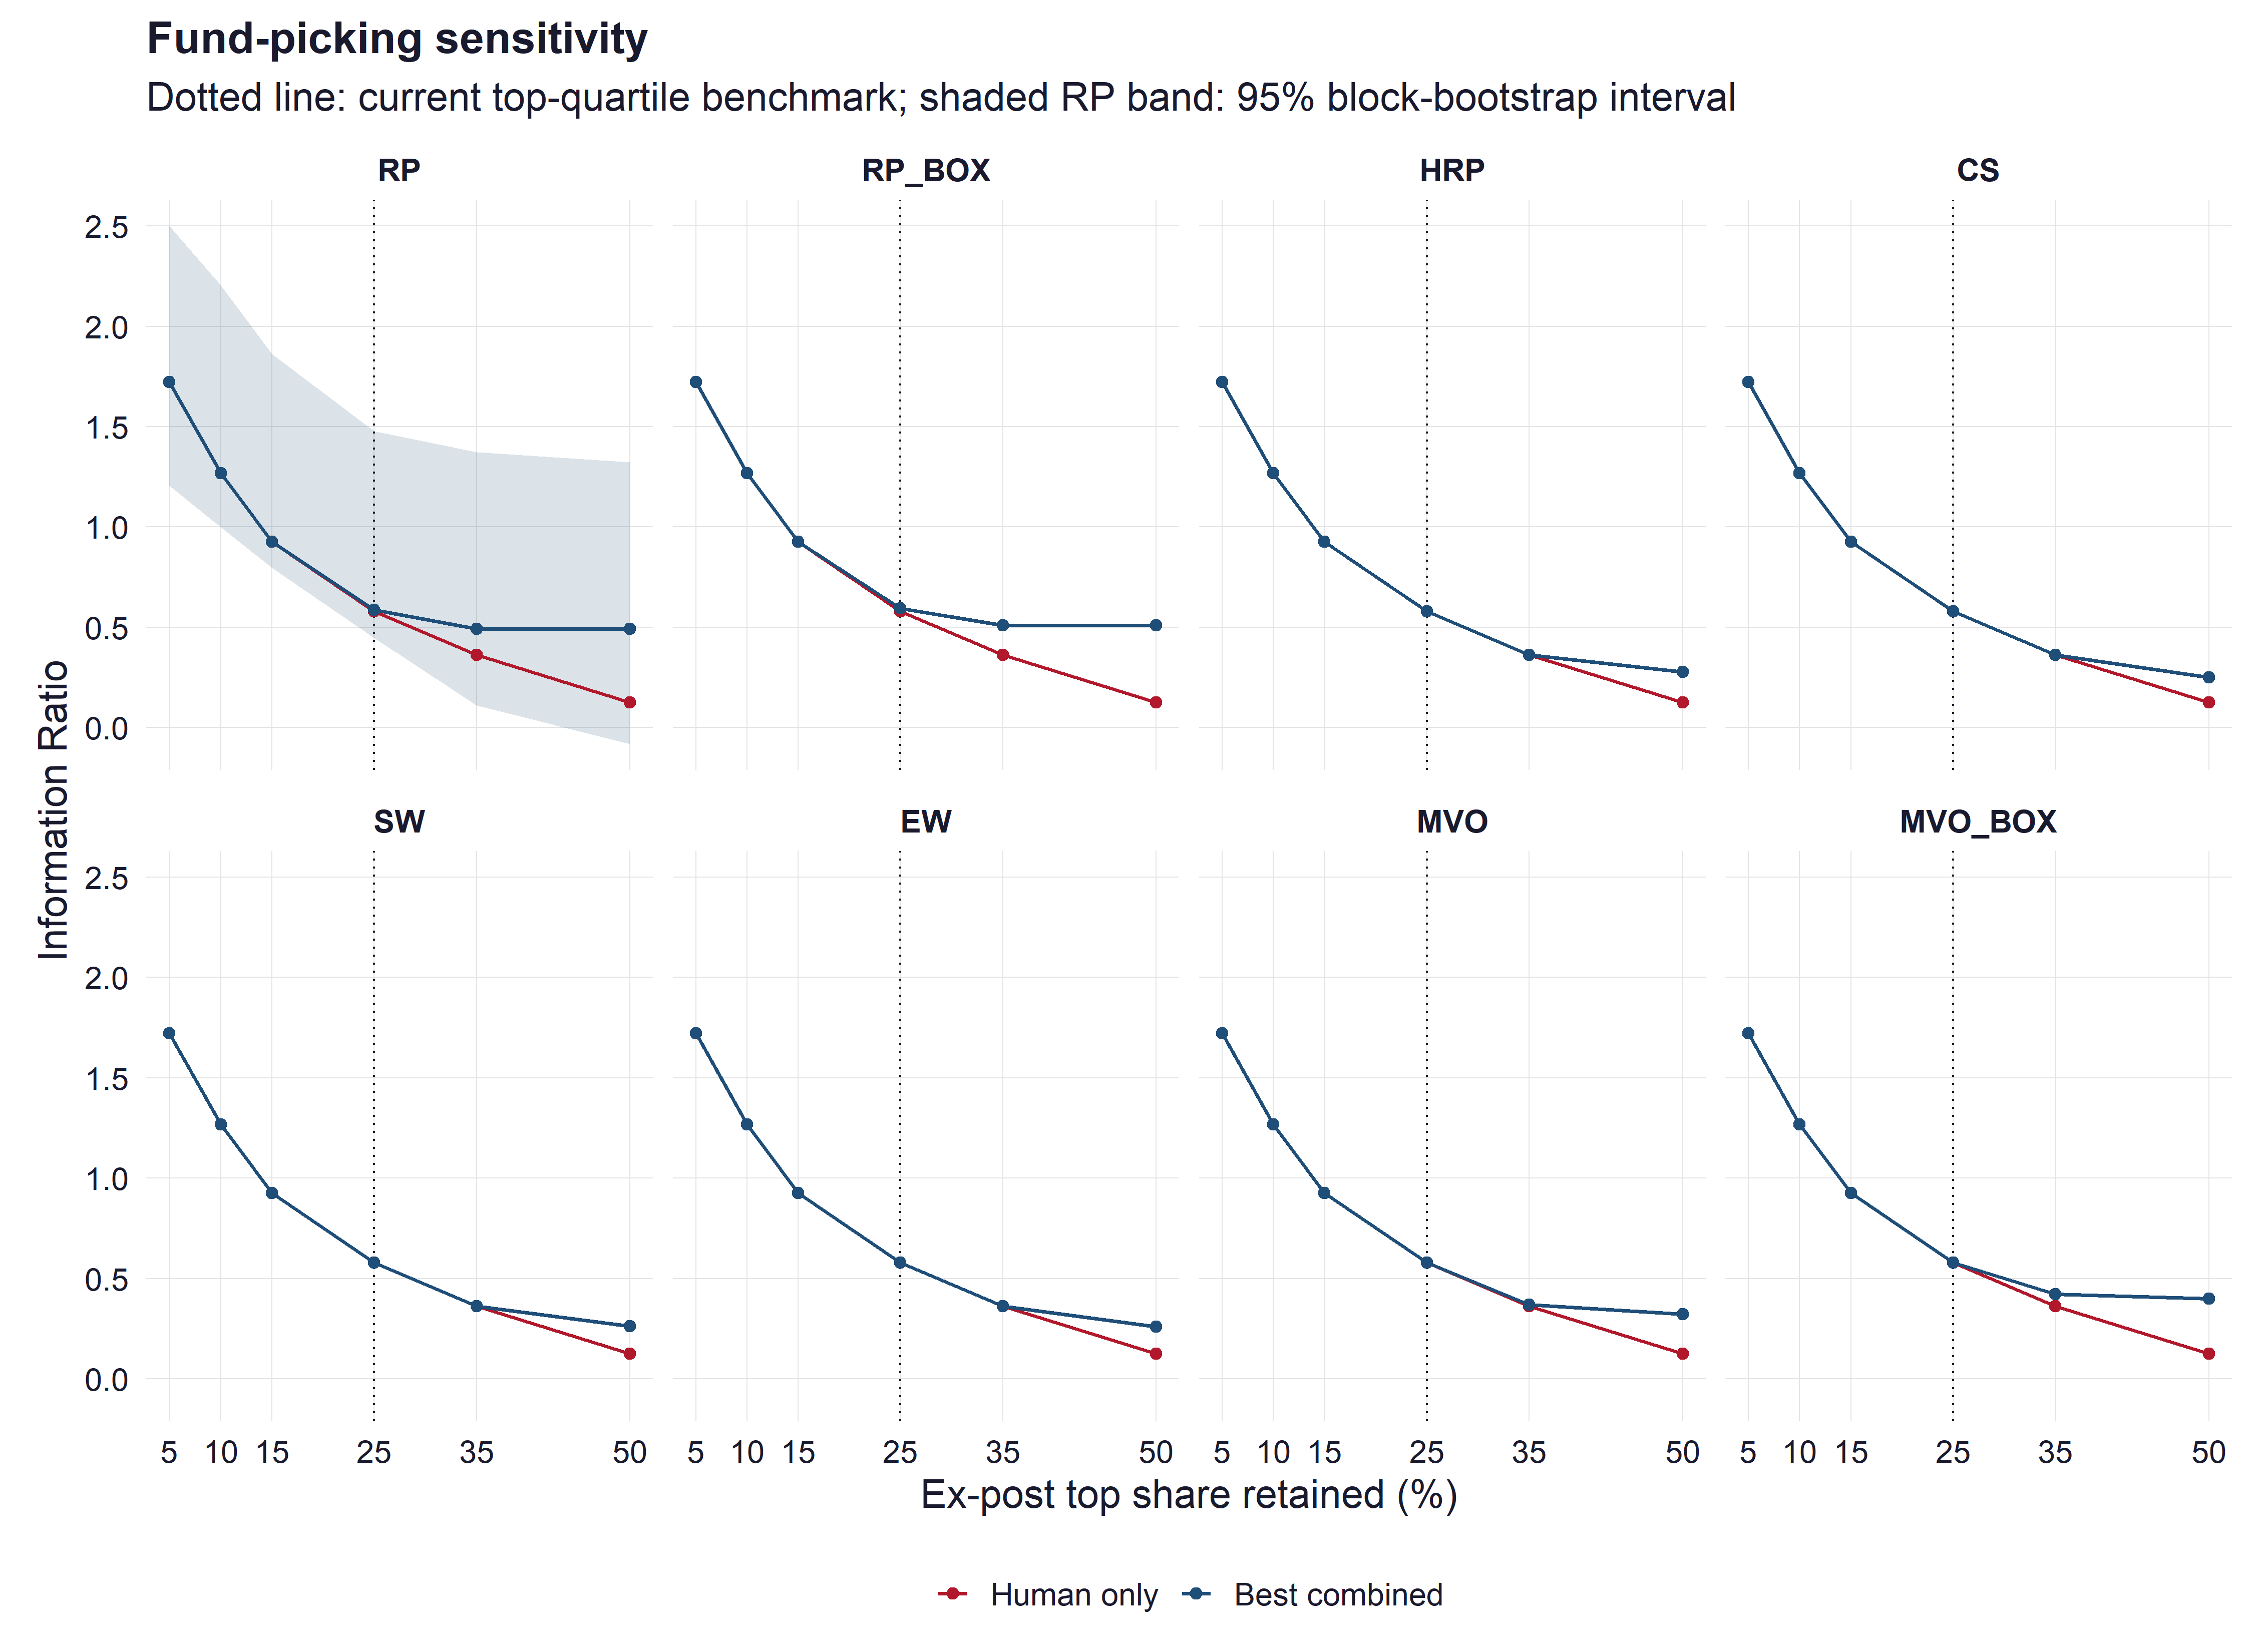
\includegraphics[width=\linewidth]{figures/fund_picker_quantile_sensitivity.png}
\label{fig:picker_quantile}
\end{figure}

\begin{figure}[htbp]
\centering
\captionsetup{
  justification=raggedright,
  labelsep=none,
  singlelinecheck=false,
  labelformat=boldlabel,
}
\caption[Figure 14: \footnotesize ]{\footnotesize \textbf{: Top-performer basket size.} Each draw samples, without replacement, a fixed equal-weight basket from the funds ranked in the ex-post top quartile and holds that basket throughout the evaluation window. For each basket size, 1,000 draws are combined with RP over a five-percentage-point weight grid. The solid line is the median attainable Information Ratio and the band spans its 5th to 95th percentiles across basket draws. The dashed line is standalone RP; the final point includes every top-quartile fund. The band therefore measures fund-selection dispersion, not time-series sampling uncertainty, and the ex-post top-quartile restriction makes the exercise an oracle diversification benchmark.}
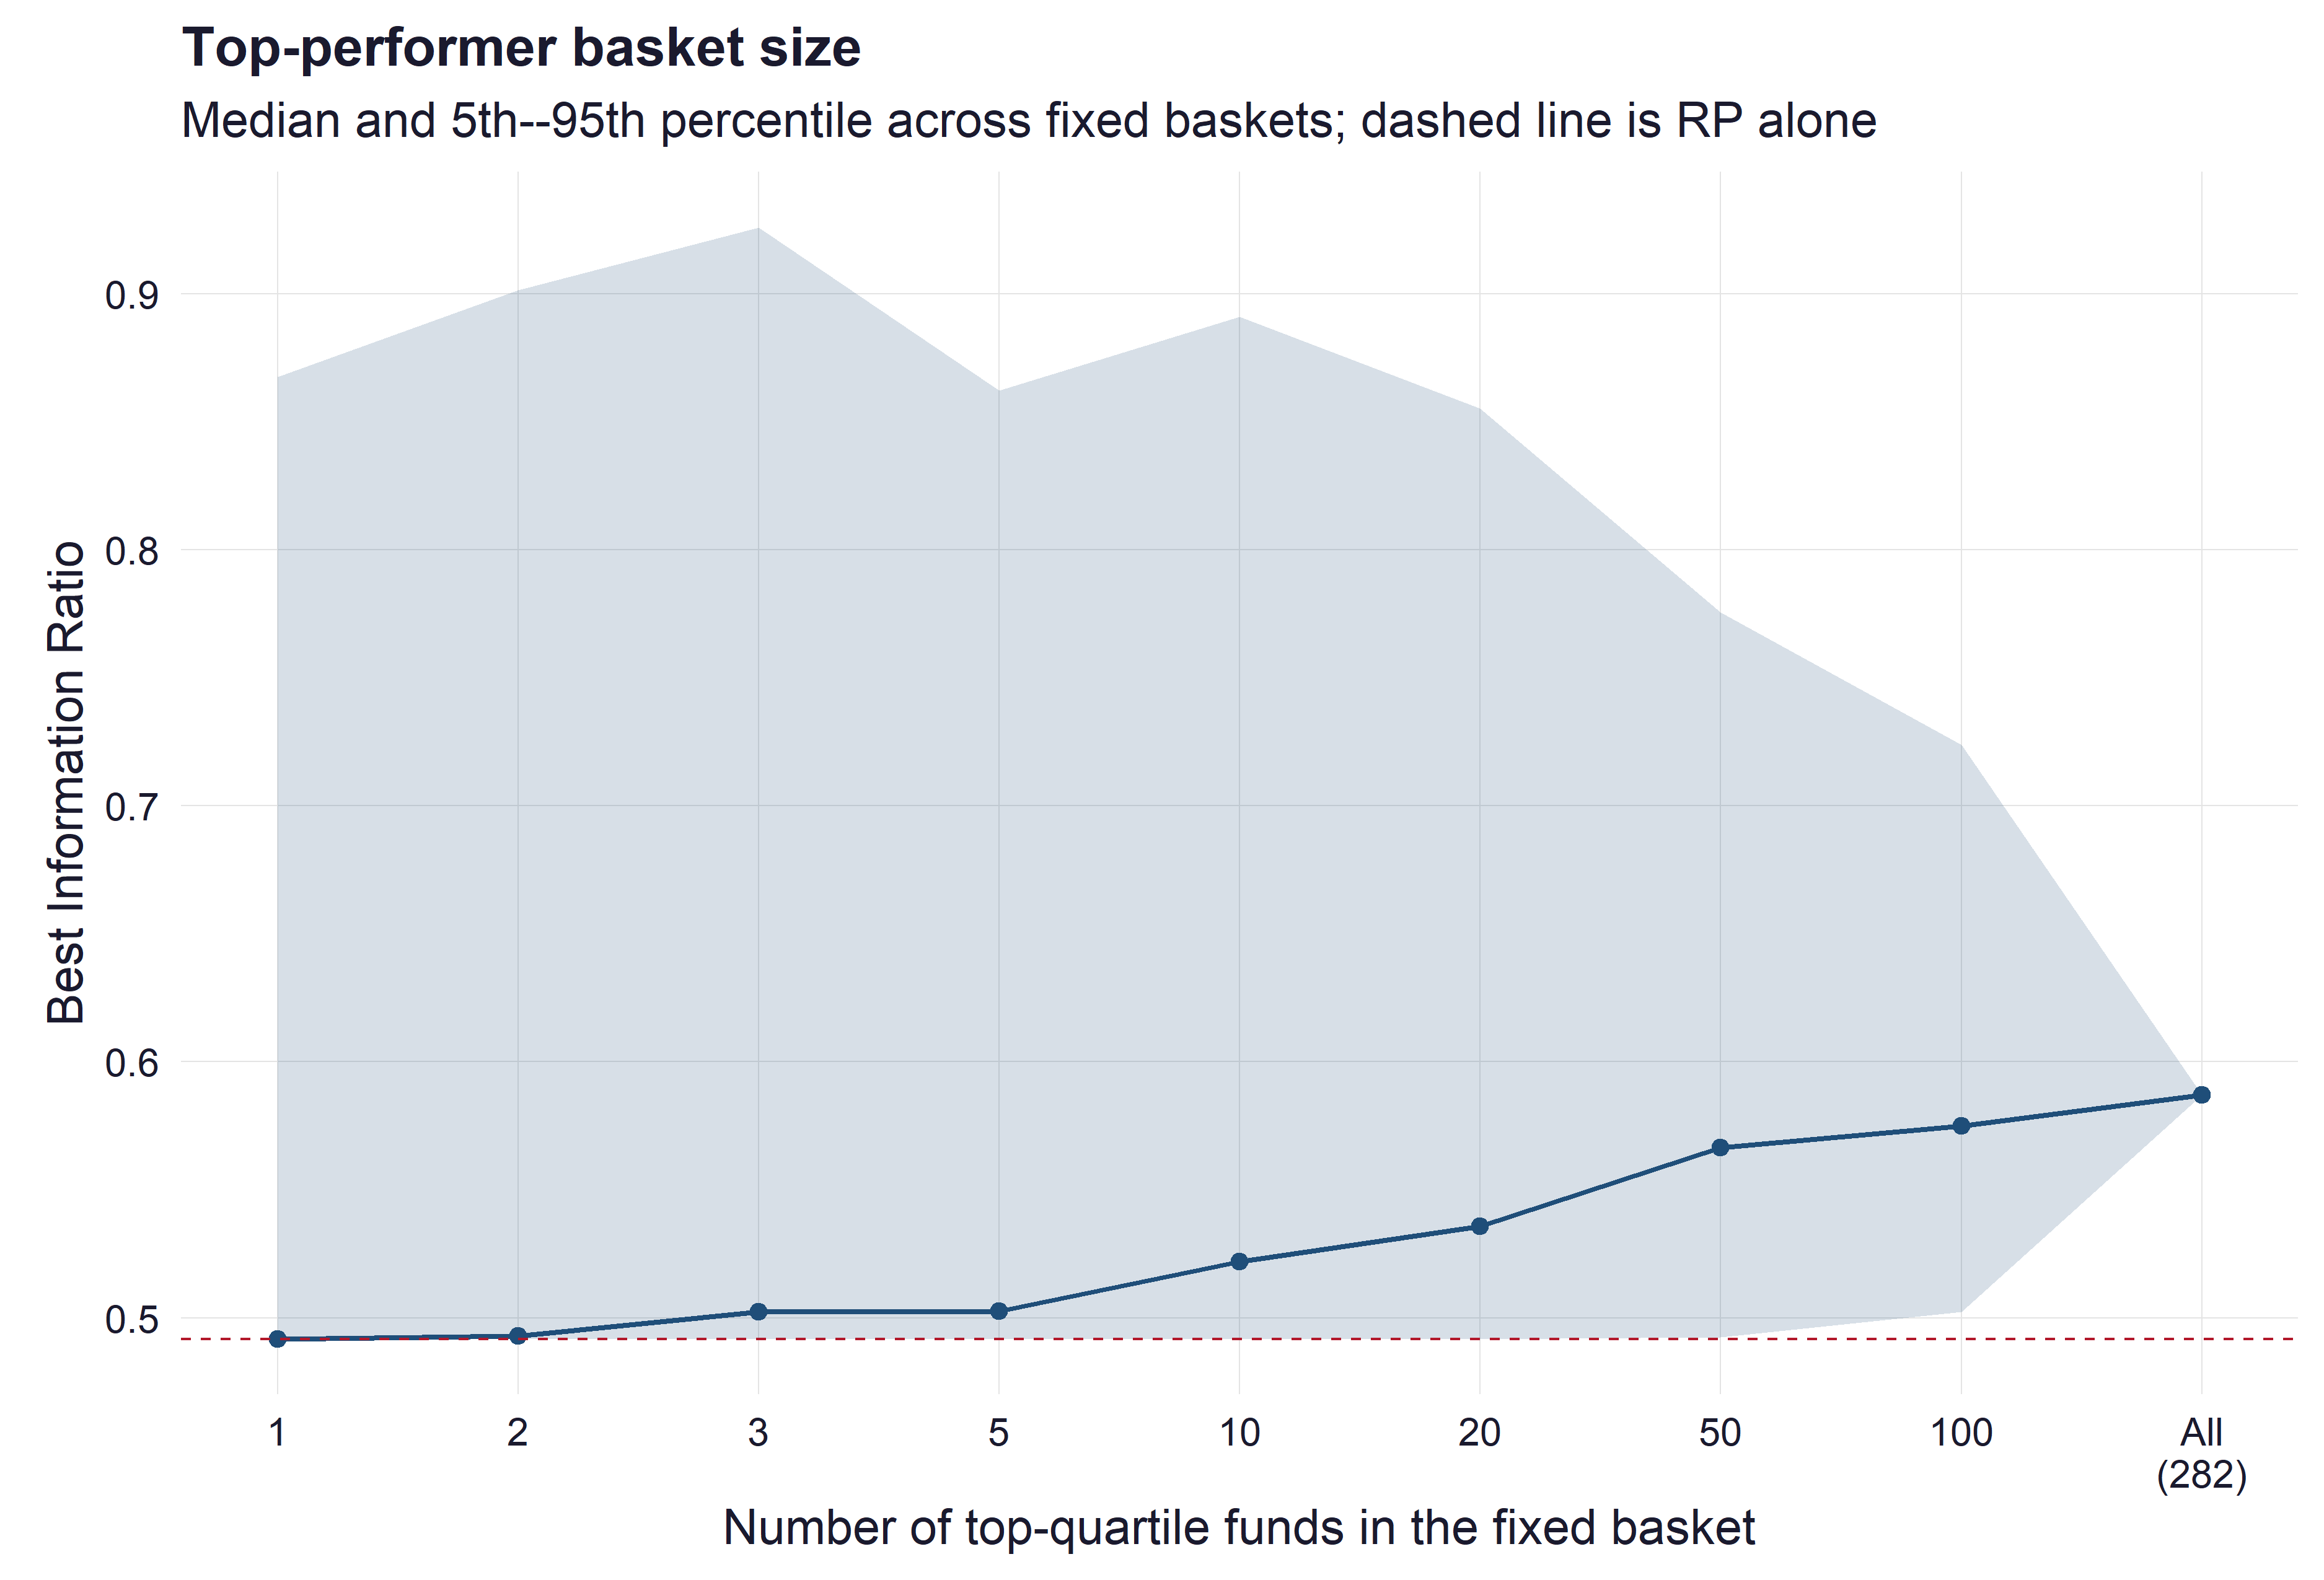
\includegraphics[width=\linewidth]{figures/fund_picker_basket_size.png}
\label{fig:picker_basket}
\end{figure}

\begin{figure}[htbp]
\centering
\captionsetup{
  justification=raggedright,
  labelsep=none,
  singlelinecheck=false,
  labelformat=boldlabel,
}
\caption[Figure 15: \footnotesize ]{\footnotesize \textbf{: Fund-picker precision.} For basket sizes 4, 8, 20 and 40, a controlled fraction of funds is sampled without replacement from the ex-post top quartile and the remainder from the other eligible funds. Each cell summarizes 500 fixed equal-weight baskets. Every basket is combined with RP over a five-percentage-point weight grid. Cell colour and the first number report the median incremental Information Ratio relative to the better standalone RP or human basket; the parenthesized number is the fraction of draws with a positive increment. The exercise calibrates how accurately an investor must identify eventual winners, but because winner status uses the full window it is not an implementable picker.}
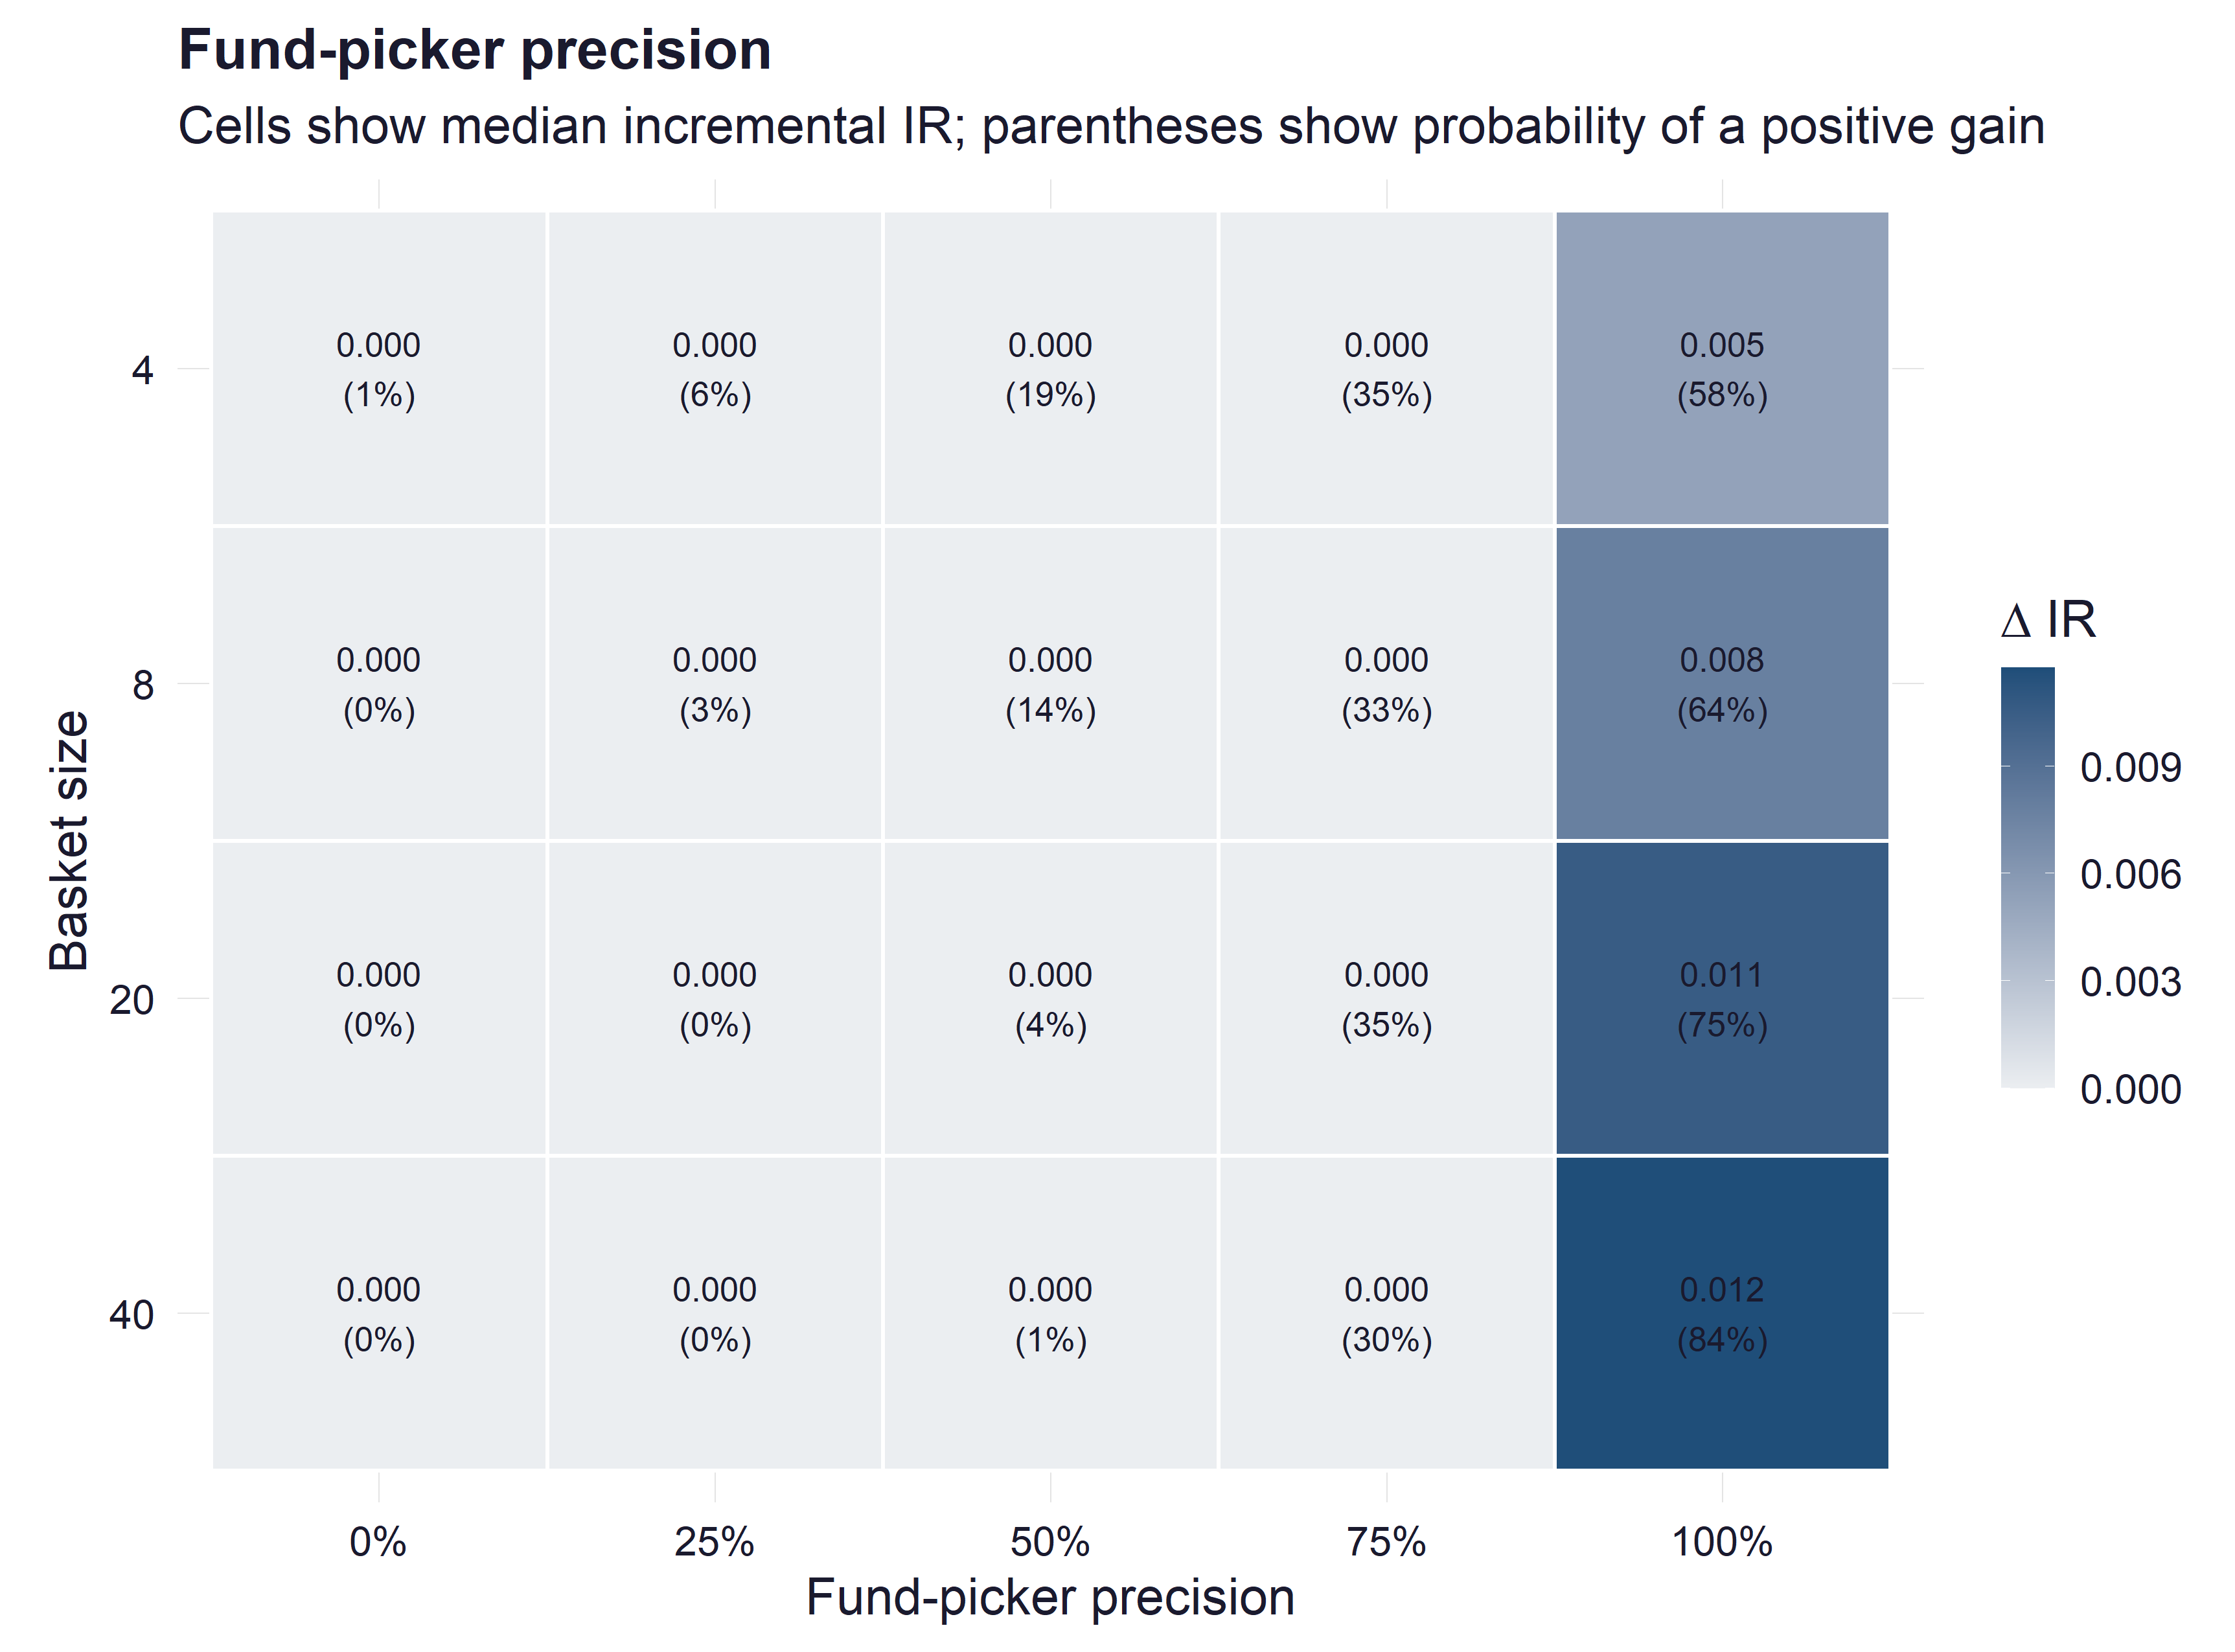
\includegraphics[width=\linewidth]{figures/fund_picker_precision.png}
\label{fig:picker_precision}
\end{figure}









% Retained only as source provenance; excluded from the compiled manuscript.
\iffalse
\label{vardefinitions_legacy}
      \vspace{1em} % Add some vertical space if needed
\begin{table}[pt]
\captionsetup{
  justification=raggedright, % Left-align the caption
  labelsep=none,
  singlelinecheck=false, % Allow multi-line captions
  labelformat=boldlabel, % Use the custom label format
}
\renewcommand{\arraystretch}{1.25}
\caption[Table 1: \footnotesize ]{\footnotesize \\ \textbf{Variables Definitions - Part 1}. This table shows predictors, their respective theme and related study.}  
\footnotesize % Reduce font size further
\begin{tabularx}{\linewidth}{>{\raggedright\arraybackslash}m{3cm}>{\raggedright\arraybackslash}m{3.5cm}>{\raggedright\arraybackslash}m{4cm}>{\raggedright\arraybackslash}m{4cm}}
\hline
\multirow{2}{*}{Definition} & \multirow{2}{*}{Name} & \multirow{2}{*}{Citation} & \multirow{2}{*}{Cluster} \\
& & & \\
\hline
6m Acceleration & $acceleration\_6m$ & Gettleman and Marks (2006) & Momentum \\
6m Alpha & $alpha\_6m$ & Hünh and Scholz (2018) & Momentum \\
12m Alpha & $alpha\_12m$ & As above & Momentum \\
Asset Growth & $assets\_gr3y$ & Cooper et al. (2008) & Investment  \\
Asset Turnover & $asset\_turnover\_12m$ & Haugen and Baker (1996) & Quality \\
Assets Yield & $assets\_yield$ & Fama and French (1992) & Value \\
Book Growth & $be\_gr3y$ & Richardson et al. (2005) & Investment \\
Book Leverage & $book\_lev$ & Fama and French (1992) & Leverage \\
Beta - Market & $beta\_mrkt\_36m$ & Fama and MacBeth (1973) & Low Risk \\
Book Yield & $book\_yield$ & Rosenberg et al. (1985) & Value \\
CAPEX Growth & $capex\_gr3y$ & Anderson and Garcia-Feijoo (2006) & Investment \\
Cash Flow Margin & $cf\_mrg\_12m$ & Huang (2009) & Profitability \\
Cash Flow Volatility & $cf\_mrg\_12m\_sd\_3y$ &  As above & Quality \\
Commodities Price Surprise\footnote{} & $commodities\_sur\_3y$ & Brooks et al. (2016) & Macro \\
Correlation - Market & $corr\_mrkt\_36m$ & Asness et al. (2020) & Low Risk \\
Current Ratio & $curr\_ratio$ & Ou and Penman (1989) & Quality \\
Debt-to-Market Equity & $debt.me$ & Penman et al. (2007) & Leverage \\
Dividend Yield & $dps\_yield$ & Litzenberger and Ramaswamy (1982) & Value \\
Dividend Stability & $dy\_med\_36m$ & Owain et al. (2000) & Value \\
Dividend Growth & $dps\_12m\_gr3y$ & Maio and Santa-Clara (2015)  & Profit Growth \\
\hline
\end{tabularx}
\label{mostcitedarticles}
\end{table}

      \vspace{1em} % Add some vertical space if needed
\begin{table}[pt]
\captionsetup{
  justification=raggedright, % Left-align the caption
  labelsep=none,
  singlelinecheck=false, % Allow multi-line captions
  labelformat=boldlabel, % Use the custom label format
}
\renewcommand{\arraystretch}{1.25}
\caption[Table 1: \footnotesize ]{\footnotesize \\ \textbf{Variables Definitions - Part 2}. This table shows predictors, their respective theme and related study.}  
\footnotesize % Reduce font size further
\begin{tabularx}{\linewidth}{>{\raggedright\arraybackslash}m{3cm}>{\raggedright\arraybackslash}m{3.5cm}>{\raggedright\arraybackslash}m{4cm}>{\raggedright\arraybackslash}m{4cm}}
\hline
\multirow{2}{*}{Definition} & \multirow{2}{*}{Name} & \multirow{2}{*}{Citation} & \multirow{2}{*}{Cluster} \\
& & & \\
\hline
Dividend Surprise & $dps\_12m\_sur3y$ & Guo et al. (2023) & Profit Growth \\
EBITDA Yield & $ebitda\_yield$ & Loughran and Wellman (2011) & Value\\
Earnings Yield & $eps\_yield$ & Basu (1983) & Value\\
Earnings Growth & $eps\_12m\_gr3y$ & Asness et al. (2018) & Profit Growth\\
Earnings Surprise & $eps\_12m\_sur3y$ & Foster et al. (1984) & Profit Growth\\
Equity Ney-Payout & $eqnpo\_12m$ & Daniel and Titman (2006) & Value \\
Fixed Costs to Sales & $fixed\_costs.sales$ & Gorodnichenko and Weber (2016) & Leverage \\
Free-Cash Flow to Invested Capital & $fcf.invcap\_12m$ & Bouchard et al. (2019) & Profitability \\
Free Cash-Flow to Invested Capital Growth & $fcf.invcap\_12m\_gr3y$ &  Bouchard et al. (2019) & Profit Growth \\
Free-Cash Flow Yield & $fcf.yield$ & Lakonishok et al. (1994) & Value \\
Free-Cash Flow Growth & $fcfps\_12m\_gr3y$ & Jansen (2021) & Profit Growth \\
Free-Cash Flow Surprise & $fcfps\_12m\_sur3y$ &  Mao and Wei (2016) & Profit Growth \\
Free-Cash Flow to Equity to Book & $fcfe.be\_12m$ & Bouchard et al. (2019) & Profitability \\
Free-Cash Flow to Equity Yield & $fcfe\_yield$ & Lakonishok et al. (1994) & Value \\
Free-Cash Flow to Firm Yield & $fcff\_yield$ &  As above & Value \\
F-Score & $fscore$ & Piotroski (2000) & Quality \\
Gross Profits to Assets & $gp.at\_12m$ & Novy-Marx (2013) & Profitability \\
Idiosyncratic Volatility & $idio\_vol\_mrkt\_ewma$ & Ali et al. (2013) & Profitability \\
\hline
\end{tabularx}
\label{mostcitedarticles}
\end{table}

      \vspace{1em} % Add some vertical space if needed
\begin{table}[pt]
\captionsetup{
  justification=raggedright, % Left-align the caption
  labelsep=none,
  singlelinecheck=false, % Allow multi-line captions
  labelformat=boldlabel, % Use the custom label format
}
\renewcommand{\arraystretch}{1.25}
\caption[Table 1: \footnotesize ]{\footnotesize \\ \textbf{Variables Definitions - Part 3}. This table shows predictors, their respective theme and related study.}  
\footnotesize % Reduce font size further
\begin{tabularx}{\linewidth}{>{\raggedright\arraybackslash}m{3cm}>{\raggedright\arraybackslash}m{3.5cm}>{\raggedright\arraybackslash}m{4cm}>{\raggedright\arraybackslash}m{4cm}}
\hline
\multirow{2}{*}{Definition} & \multirow{2}{*}{Name} & \multirow{2}{*}{Citation} & \multirow{2}{*}{Cluster} \\
& & & \\
\hline
Illiquidity & $mean\_volfin\_3m$ & Dino (2023) & Size \\
Interest Rate Differential Surprise & $rate\_diff\_sur5y$ & Lioui and Maio (2014)  & Macro \\
Interest Rate Surprise & $realrate\_sur5y$ &  As above & Macro \\
Long-term Reversal & $ret\_60m\_l1y$ & DeBondt and Thaler (1985) & Reversal \\
Market Cap & $mkt\_cap$ & Banz (1981) & Size \\
Max Return 1m & $max\_ret\_1m$ & Bali et al. (2011) & Momentum \\   
Monthly Inflation Surprise & $ipca\_monthly\_sur\_5y$ & Duarte (2013) & Macro \\
Net Margin & $net\_mrg\_12m$ & Soliman (2008) & Profitability \\
Net Margin Growth & $net\_mrg\_12m\_gr3y$ & Asness et al. (2018) & Profit Growth \\
Net Margin Volatility & $net\_mrg\_12m\_sd\_3y$ & Francis et al. (2004) & Quality \\
Net Operating Assets Growth  & $noa\_gr3y$ & Richardson et al. (2005) & Investment \\
Net Operating Assets to Assets & $noa.at$ & Hirschleifer et al. (2004) & Accruals \\
Operating Accruals & $oaccruals.at$ & Sloan (1996) & Accruals \\
Operating Cash-Flow Yield & $ocf\_yield$ & Lakonishok et al. (1994) & Value \\
Operating Cash-Flow to Assets & $ocf\_at\_12m$ &  Bouchard et al. (2019) & Profitability \\
Operating Leverage & $ope\_lev$ & Novy-Marx (2013) & Quality \\
Payout & $payout\_12m$ & Asness et al. (2018) & Quality \\
\hline
\end{tabularx}
\label{mostcitedarticles}
\end{table}

      \vspace{1em} % Add some vertical space if needed
\begin{table}[pt]
\captionsetup{
  justification=raggedright, % Left-align the caption
  labelsep=none,
  singlelinecheck=false, % Allow multi-line captions
  labelformat=boldlabel, % Use the custom label format
}
\renewcommand{\arraystretch}{1.25}
\caption[Table 1: \footnotesize ]{\footnotesize \\ \textbf{Variables Definitions - Part 4}. This table shows predictors, their respective theme and related study.}  
\footnotesize % Reduce font size further
\begin{tabularx}{\linewidth}{>{\raggedright\arraybackslash}m{3cm}>{\raggedright\arraybackslash}m{3.5cm}>{\raggedright\arraybackslash}m{4cm}>{\raggedright\arraybackslash}m{4cm}}
\hline
\multirow{2}{*}{Definition} & \multirow{2}{*}{Name} & \multirow{2}{*}{Citation} & \multirow{2}{*}{Cluster} \\
& & & \\
\hline
Price to Max Price 12m & $prc\_highprice\_12m$ & George and Hwang (2004)  & Reversal \\
Residual Momentum & $mom\_res\_12m$ & Blitz, Huij and Martens (2011) & Momentum \\
Return on Equity & $roe\_12m$ & Haugen and Baker (1996)  & Profitability \\
Return on Equity - Quarterly & $roe\_3m$ & As above & 
Profitability \\
Return on Equity Growth & $roe\_12m\_gr3y$ & Asness et al. & Profit Growth \\
Return on Equity - Volatility & $roe\_12m\_sd\_3y$ & Francis et al. (2004) & 
Profitability \\
Sales Yield & $sales\_yield$ & Barbee et al. (1996) & Value \\
Sales Growth & $sps\_12m\_gr3y$ & Abarbanell and Bushee (1998) & Profit Growth \\
Sales Surprise & $sps\_12m\_sur\_3y$ & Jegadeesh and Livnat (2006) & Profit Growth \\
Seasonality Years 1-7 & $seas\_1\_7$ & Heston and Sadka (2008) & Seasonality \\
Seasonality Years 2-5 & $seas\_2\_5$ & As above & Seasonality \\
Sector Book Yield & $book\_yield\_sector$ & Asness et al. (2000) & Value \\
Sector-Adjusted Book Yield & $book\_yield\_within$ & As above & Value  \\
Sector Dummies & $'sector\_name'$ & Gu et al. (2020) & Sector \\
Sector Operating Cash-Flow Yield & $ocf\_yield\_sector$ & Asness et al. (2000) & Value \\
Sector-Adjusted Operating Cash-Flow Yield & $ocf\_yield\_within$ & As above & Value \\
\hline
\end{tabularx}
\label{mostcitedarticles}
\end{table}



      \vspace{1em} % Add some vertical space if needed
\begin{table}[pt]
\captionsetup{
  justification=raggedright, % Left-align the caption
  labelsep=none,
  singlelinecheck=false, % Allow multi-line captions
  labelformat=boldlabel, % Use the custom label format
}
\renewcommand{\arraystretch}{1.25}
\caption[Table 1: \footnotesize ]{\footnotesize \\ \textbf{Variables Definitions - Part 5}. This table shows predictors, their respective theme and related study.}  
\footnotesize % Reduce font size further
\begin{tabularx}{\linewidth}{>{\raggedright\arraybackslash}m{3cm}>{\raggedright\arraybackslash}m{3.5cm}>{\raggedright\arraybackslash}m{4cm}>{\raggedright\arraybackslash}m{4cm}}
\hline
\multirow{2}{*}{Definition} & \multirow{2}{*}{Name} & \multirow{2}{*}{Citation} & \multirow{2}{*}{Cluster} \\
& & & \\
\hline

Sector-Adjusted Size & $size\_within$ & Asness et al. (2000) & Size \\
Sector Sharpe 6m & $sharpe\_6m\_sector$ & Moskowitz and Grinblatt (1999) & Momentum \\
Sharpe 12m & $sharpe\_12m$ & Daniel and Moskowitz (2016) & Momentum \\
Sharpe 6m & $sharpe\_6m$ & As above & Momentum \\
Sharpe Ewma & $sharpe\_ewma$ & As above & Momentum \\
Skewness 1y & $skew\_1y$ & Bali et al. (2016)  & Skewness \\
Skewness 3y & $skew\_3y$ & As above & Skewness \\
Short-term Reversal & $ret\_1m$ & Jegadeesh (1990) & Reversal \\
Volatility of Liquidity & $sd\_volfin\_6m$ & 
Chordia et al. (2001) & Size \\
Tobin Q & $tobin\_q$ & Freyberger (2020) & Value \\
Total Debt Growth & $total\_debt\_gr3y$ & Lyandres et al. (2008) & Leverage \\
Turnover & $turnover\_3m$ & Datar et al. (1998) & Size \\
Trading Volume & $mean\_volfin\_3m$ & Chordia et al. (2001) & Size \\
Unexplained Volume & $qtt\_1m\_sur\_3y$ & Garfinkel (2009) & Size \\
Volatility & $vol\_12m$ & Ang et al. (2006)  & Low Risk \\
Yearly Inflation Surprise & $ipca\_yearly\_sur\_5y$ & Duarte (2013) & Macro \\
\hline
\end{tabularx}
\label{mostcitedarticles}
\end{table}

\fi




\end{appendices}
\end{document}

%\endinput
%%
%% End of file `elsarticle-template-harv.tex'.
